\documentclass{article}
\usepackage{amsthm,amsmath,amsfonts,natbib,mathtools,custom_math}
\usepackage[hscale=0.7,vscale=0.8]{geometry}

\usepackage{subfigure}
\usepackage{graphicx}
\usepackage{hyperref}
\usepackage{authblk}

\usepackage{yhmath}

\bibliographystyle{plainnat}

\title{Variable Selection in Convex Function Estimation}

%\author{
%Min Xu, Minhua Chen, John Lafferty
%}

\author[1]{Min Xu}
\author[2,3]{Minhua Chen}
\author[2,3]{John Lafferty}

\affil[1]{Machine Learning Department, Carnegie Mellon University}
\affil[2]{Department of Statistics, University of Chicago}
\affil[3]{Department of Computer Science, University of Chicago}


% ENVIRONMENTS
\numberwithin{equation}{section}
\theoremstyle{plain}
\newtheorem{theorem}{Theorem}[section]
\newtheorem{corollary}{Corollary}[section]
\newtheorem{proposition}{Proposition}[section]
\newtheorem{lemma}{Lemma}[section]
\newtheoremstyle{remark}{\topsep}{\topsep}%
     {\normalfont}% Body font
     {}           % Indent amount (empty = no indent, \parindent = para indent)
     {\bfseries}  % Thm head font
     {.}          % Punctuation after thm head
     {.5em}       % Space after thm head (\newline = linebreak)
     {\thmname{#1}\thmnumber{ #2}\thmnote{ #3}}% Thm head spec
\theoremstyle{remark}
\newtheorem{remark}{Remark}[section]
\newtheorem{example}{Example}[section]
\newtheorem{assumption}{Assumption}[section]
\newtheorem{definition}{Definition}[section]



\begin{document}

% min's macros
\mathchardef\mh="2D

% John's macros
\def\X{\mathcal{X}}
\def\comma{\unskip,~}
\def\truep{p^*}
\def\div{\|\,}
\long\def\comment#1{}
\def\reals{{\mathbb R}}
\def\P{{\mathbb P}}
\def\E{{\mathbb E}}
\def\Cov{\mathop{\text{Cov}}}
\def\supp{\mathop{\text{supp}\kern.2ex}}
\def\argmin{\mathop{\text{\rm arg\,min}}}
\def\arginf{\mathop{\text{\rm arg\,inf}}}
\def\argmax{\mathop{\text{\rm arg\,max}}}
\let\tilde\widetilde
\def\csd{${}^*$}
\def\mld{${}^\dag$}
\def\dos{${}^\ddag$}
\def\W{\widetilde Y}
\def\Z{\widetilde X}
\let\hat\widehat
\let\tilde\widetilde
\def\given{{\,|\,}}
\def\ds{\displaystyle}
\def\bs{\backslash}
\def\1{{(1)}}
\def\2{{(2)}}
\def\pn{{(n)}}
\def\ip{{(i)}}
\def\Xbar{\overline{X}}
\def\except{\backslash}
\def\npn{\mathop{\textit{NPN\,}}}
\def\i{{(i)}}
\def\cE{{\mathcal{C}}}
\def\cM{{\mathcal{M}}}
\def\cF{{\mathcal{F}}}
\def\cP{{\mathcal{P}}}
\def\cG{{\mathcal{G}}}
\def\tr{\mathop{\text{tr}}}
\long\def\comment#1{}
\def\ti#1{#1}
\def\titi#1{\textit{#1}}
\def\cram{{\sc cram}}
\def\spam{{\small\sc SpAM}}
\def\diag{\mathop{\rm diag}}
\def\ones{\mathbf{1}}
\def\threebars{\mbox{$|\kern-.25ex|\kern-.25ex|$}}
\def\fatnorm#1{\threebars #1 \threebars}
\def\rank{\mathop{\rm rank}}
\def\S{\mathcal{S}}
\def\H{\mathcal{H}}
\def\K{{K}}
\def\rank{\mathop{\rm rank}}
\def\half{{1/2}}
\def\Y{\mathbb{Y}}
\def\M{\mathbb{M}}
\def\F{\mathbb{F}}
\def\pinv{{-1}}
%\def\ones{\mathds{1}}
%\def\ones{1}
\def\Res{Z}
\def\Proj{P}
\def\cN{{\mathcal N}}
\def\cT{{\mathcal H}}
\def\coloneqq{:=}
\def\mathbf#1{\mbox{\boldmath $#1$}} 
\def\bar#1{\overline{#1}}




\maketitle

\begin{abstract}
We consider the problem of estimating a convex function of several variables from noisy values of the function at a finite sample of input points. 
\end{abstract}
\vskip10pt

% \tableofcontents

\section{Introduction}


Shape restrictions such as monotonicity, convexity, and concavity
provide a natural way of limiting the complexity of many statistical
estimation problem.  Shape-constrained estimation is not as well
understood as more traditional nonparametric estimation involving
smoothness constraints.  For instance, as of this writing, the minimax
rate of convergence for multivariate convex regression has yet to be
rigorously established in full generality.  Even the one-dimensional
case is challenging, and has been of recent interest
\citep{guntusen:13}.

In this paper we study the problem of variable selection in convex
regression.  Assuming that the regression function is convex and
sparse, our goal is to identify the relevant variables.  We show that
it suffices to estimate a sum of $p$ one-dimensional convex functions,
leading to significant computational and statistical advantages.  This
is in contrast to general nonparametric regression, where fitting an
additive model can result in false negatives.  Our approach is based
on a two-stage quadratic programming procedure.  In the first stage,
we fit an convex additive model, imposing a sparsity penalty.  In the
second stage, we fit a concave function on the residual for each
variable.  As we demonstrate, this perhaps non-intuity second stage is
in general necessary.  Our first result is that this procedure is
faithful in the population setting, meaning that it results in no
false negatives, under mild assumptions on the density of the
covariates.  Our second result is a finite-sample statistical analysis
of the procedure, where we upper bound the statistical rate of
convergence.  Each stage of the method requires quadratic programming.
An additional contribution is to show how these quadratic programs can
be forumlated to be more scalable.  Simulations demonstrate the method
performs in a manner that is consistent with our analysis.

Estimation of convex functions arises naturally in several
applications.  Examples include geometric programming \citep{Boyd04},
computed tomography \citep{Prince:90}, target reconstruction
\citep{Lele:92}, image analysis \citep{Golden:06} and circuit design
\citep{Hannah:12}.  Other applications include queuing theory
\citep{Chen:01} and economics, where it is of interest to estimate
concave utility functions \citep{Pratt:68}.  See \cite{Lim:12} for
other applications.  
Beyond cases where the assumption of convexity is
natural, the convexity assumption can be attractive as a
tractable, nonparamametric relaxation of the linear model.  

Variable selection in general nonparametric regression or function
estimation is a notoriously difficult problem. \citet{lafferty2008rodeo} develop a greedy procedure for
adjusting bandwidths in a local linear regression estimator,
and show that the procedure achieves the minimax rate
as if the relevant variables were isolated in advance.
But the method only provably scales to dimensions $p$ that 
grow logarithmically in the sample size $n$, so that $p = O(\log n)$.  Note that this
is the opposite of the high dimensional scaling behavior
known to hold for sparsity selection in linear models
using $\ell_1$ penalization, where the sample size $n$
is logarithmic in the dimension $p$. \citet{bertin:08}
develop an optimization-based approach in
the nonparametric setting, applying the lasso
in a local linear model at each test point.  Here again,
however, the method only scales as $p = O(\log n)$,
the low-dimensional regime.
An approximation theory approach to the same
problem is presented in \cite{devore:11}, 
using techniques based on hierarchical hashing schemes,
similar to those used for ``junta'' problems \cite{mossel:04}.
Here it is shown that the sample complexity scales as $n > \log p$ 
if one adaptively selects the points on
which the high-dimensional function is evaluated.

\citet{dalalyan:12} show that the exponential scaling $p=O(\log n)$ is achievable if the underlying function is assumed to be smooth with respect to a Fourier basis. They also give
support for the intrinsic difficulty of variable
selection in nonparametric regression, giving lower bounds 
showing that sparsistency is not possible if $n < \log p$ or if $n <
\exp s$, where $s$ is the number of relevant variables.
Variable selection over kernel classes is studied
by \citet{Kolch:10}.  

Perhaps most closely related to the present work, is the framework
studied by \cite{Raskutti:12} for sparse additive models, where sparse
regression is considered under an additive assumption, with each
component function belonging to an RKHS.  An advantage of working over
an RKHS, in contrast to the other papers mentioned above, is that
nonparametric regression with a sparsity-inducing regularization penalty can be
formulated as a finite dimensional convex cone optimization.
On the other hand, 
smoothing parameters for the component Hilbert spaces
must be chosen, leading to extra tuning parameters
that are difficult to select in practice.  In addition, 
the additive model must be assumed to
be correct for sparsistent variable selection.

An attraction of the convex function estimation framework we consider
in this paper is that the additive model can be used for convenience,
without assuming it to actually hold.  While nonparametric, the
problem is naturally formulated using finite dimensional convex
optimization, but with no additional tuning parameters.  As we show
below, our method scales to high dimensions, with a dependence on the
intrinsic dimension $s$ that scales polynomially, rather than
exponentially as in the general case analyzed in \cite{dalalyan:12}.



%* Laetitia Comminges, Arnak S. Dalalyan 
%Tight conditions for consistency of variable selection 
%In the context of high dimensionality. 
%Ann. Statist, 40(5), 2667-2696, 2012 
%
%Comment: They estimate the coefficient of the regression function with respect to a Fourier basis and then threshold the estimated coefficients. They prove that sparsistency is achievable so long as $n > log p$ and $n > exp(s)$. They assume that the functions are smooth with respect to the Fourier basis. The fourier coefficients however seem difficult to estimate; it appears that the knowledge of the true density is required. They also provide 
%
%
%* Bertin, K. and Lecu´e, G. (2008). Selection of variables 
%and dimension reduction in high-dimensional non-parametric 
%regression. Electron. J. Stat. 2 1224–1241 
%
%Comment: They assume Holder smoothness and use multiple L1 regularized local polynomial smoothing to detect the sparsity pattern. They require that $p < log n$.
%
%
%* "Approximation of Functions of Few Variables in High Dimensions" 
%by DeVore, Petrova and Wojtaszczyk. 
%
%Comment: They show that variable selection under a scaling of
%


%Variable selection for nonparametric
%regression under smoothness constraints is difficult without
%making additional strong assumptions. 
%\cite{lafferty2008rodeo} show that computationally
%efficient, near minimax-optimal estimation is possible, but in ambient
%dimensions that scale only as $p = O(\log n)$; see also \cite{BertinLecue}.  This is in contrast
%to the $p=O\bigl(e^{n^c}\bigr)$ scaling enjoyed by sparse linear
%models \cite{Wain:09a}. \citet{dalalyan:12} achieve exponential scaling $p=O(e^n)$
%under certain Fourier smoothness conditions, but require
%that the number of relevant variables $s$ must be less than $\log n$.
%
%Approximating the regression function by a sum of one-dimensional
%functions, known as sparse additive models \citep{Ravikumar:09}, is a
%practical alternative to fully nonparametric function estimation.  
%Sparse additive models have been further studied in by \cite{Meier09},
%and by \cite{Raskutti:12}.  But 
%the additive assumption is limited.  In particular, the natural idea
%of first selecting the single variable effects, then the pairwise
%effects, and so on, does not in general lead to consistent variable
%selection.  In other words, the general nonparametric model is not
%additively faithful.  Remarkably, the additional assumption of
%convexity does lead to consistent variable selection, as we show
%here. In addition, we show that the high dimensional scaling $n =
%O\big(\textrm{poly}(s) \log p\big)$ is achievable for sparse convex
%additive models. Thus, with respect to variable selection, the
%geometric convexity constraint is quite different from the smoothness
%constraints imposed in traditional nonparametric regression.
%

In the following section we give a high-level summary of our technical
results, including additive faithfulness, variable selection 
consistency, and high dimensional scaling.  In Section~X...



% DO NOT CHANGE; RefTex variables -minx

%%% Local Variables: ***
%%% mode:latex ***
%%% TeX-master: "paper.tex" ***
%%% End: ***

\section{Related Work}
\def\x{\mathbf{x}}

\section{Overview of Results}

In this section we provide a high-level description of our technical
results.  The full technical details, the precise statement of the
results, and their detailed proofs are provided in following sections.

Our main contribution is an analysis of an additive approximation for identifying
relevant variables in convex regression.  
We prove a result that shows when and how the additive approximation
can be used without introducing false negatives in the population
setting.  In addition, we develop algorithms for the efficient implementation of
the quadratic programs required by the procedure.  

We first establish some notation, to be used throughout the  paper.
If $\mathbf{x}$ is a vector, we use $\mathbf{x}_{-k}$ to denote the
vector with the $k$-th coordinate removed. If $\mathbf{v} \in \R^n$, then
$v_{(1)}$ denotes the smallest coordinate of $\mathbf{v}$ in
magnitude, and $v_{(j)}$ denotes the $j$-th smallest; $\mathbf{1}_n \in \R^n$
is the all ones vector. If $X \in \R^p$ is a random variable and $S \subset
\{1,...,p\}$, then $X_S$ is the subvector of $X$ restricted to
the coordinates in $S$. Given $n$ samples $X^{(1)},...,X^{(n)}$, we use
$\bar{X}$ to denote the sample mean. Given a random variable
$X_k$ and a scalar $x_k$, we use $\E[\,\cdot \given x_k]$ as a shorthand
for $\E[\, \cdot \given X_k = x_k]$. If we say a function is integrable, we 
mean it is Lebesgue integrable.


\subsection{Faithful screening}

The starting point for our approach is the observation that least squares
nonparametric estimation under convexity constraints is equivalent to
a finite dimensional quadratic program.  Specifically, the infinite
dimensional optimization 
\begin{align}
\begin{split}
\text{minimize} & \quad \sum_{i=1}^n (Y_i - f(\x_i))^2 \\
\text{subject to} &  \quad f:\reals^p\rightarrow\reals\ \text{is
  convex}
\end{split}
\end{align}
is equivalent to the finite dimensional quadratic
program 
\begin{align}
\label{eq:convreg}
\begin{split}
\text{minimize}_{f, \beta} & \;\; \sum_{i=1}^n (Y_i - f_i)^2 \\
\text{subject to} & \;\; f_j \geq f_i + \beta_i^T (\x_j-\x_i),\; \text{for
    all $i,j$}.
\end{split}
\end{align}
Here $f_i$ is the estimated function value $f(\x_i)$, and the vectors
$\beta_i \in \reals^d$ represent supporting hyperplanes to the
epigraph of $f$.  See \cite{Boyd04}, Section 6.5.5.
Importantly, this finite dimensional quadratic program does
not have tuning parameters for smoothing the function. 

This formulation of convex regression is subject to the curse
of dimensionality.  Moreover, attempting to select variables
by regularizing the subgradient vectors $\beta_i$ with
a group sparsity penality is not effective.  Intuitively, the reason
is that all $p$ components of the subgradient $\beta_i$
appear in every convexity constraint 
$ f_j \geq f_i + \beta_i^T (\x_j-\x_i)$; small changes to the 
subgradients may not violate the constraints.  Experimentally,
we find that regularization with a group sparsity penality
will make the subgradients of irrelevant variables 
small, but may not zero them out completely.

This motivates us to consider an additive approximation. 
%Under a convex additive model, each component of the subgradient
%appears only in the convexity constraint for
%the corresponding variable:
%\begin{equation}
%f_{ki'} \geq f_{ki} + \beta_{ki}(x_{ki'}-x_{ki}) 
%\end{equation}
%where $f_{ki} = f_{k}(x_{ki})$ and $\beta_{ki}$ is the
%subgradient at point $x_{ki}$.   
As we show, this leads to
an effective variable selection procedure.  The
shape constraints play an essential role.
For general regression, using an additive approximation for variable
selection may make errors.  In particular, the nonlinearities in the
regression function may result in an additive component being wrongly
zeroed out.  We show that this cannot happen for convex regression
under appropriate conditions.

We say that a differentiable function $f$ depends on variable $x_k$ if
$\partial_{x_k} f \neq 0$ with probability greater than zero.  An additive approximation is given by
\begin{equation}
\{f_k^*\}, \mu^* \coloneqq \argmin_{f_1,\ldots, f_p, \mu} \Bigl\{ 
             \E \Bigl( f(X) - \mu - \sum_{k=1}^p f_k(X_k)\Bigr)^2 
         \,:\, \E f_k(X_k) = 0 \Bigr\}.
\end{equation}
We say that $f$ is \textit{additively faithful} in case $f^*_k = 0$
implies that $f$ does not depend on coordinate $k$.
% We can define the support $\trm{supp}(f) \coloneqq \{ k \,:\,
% \trm{$k$ is relevant to $f$}\}$. Let $f^* = \sum_{k=1}^s$, then $f$
% is additively faith if $\trm{supp}(f) = \trm{supp}(f^*)$.
Additive faithfulness is a desirable property
since it implies that an additive approximation may allow us to 
screen out irrelevant variables.

Our first result shows that convex multivariate functions are
additively faithful
under the following assumption on the distribution of the data.
\begin{definition}
  Let $p(\mathbf{x})$ be a density supported on $[0,1]^p$.  Then $p$
  satisfies the \emph{boundary flatness condition} if for all $j$, and
  for all $\mathbf{x}_{-j}$,
\[
\frac{\partial p(\mathbf{x}_{-j} \given x_j)}{\partial x_j}  =  
\frac{\partial^2 p(\mathbf{x}_{-j} \given x_j)}{\partial x_j^2} = 0
\quad \trm{at $x_j = 0$ and $x_j = 1$}.
\]
\end{definition}

As discussed in Section~\ref{sec:additivefaithful}, this is a relatively weak condition. 
Our first result is that this condition suffices in the population
setting of convex regression.

\begin{stheorem}
  Let $p(\mathbf{x})$ be a positive density supported on $C=[0,1]^p$ that
  satisfies the boundary flatness property. If $f$ is convex with a bounded second derivative on an open set around $C$, then $f$ is additively faithful under $p$.
\end{stheorem}

% We give the full proof in Section~\ref{sec:faithful_proof} of the
% Appendix, but pause here to provide some intuition. 

Intuitively, an additive approximation zeroes out variable $k$ when, fixing $x_k$, every
``slice'' of $f$ integrates to zero. We prove this result
by showing that ``slices'' of convex
functions that integrate to zero cannot be ``glued together'' while
still maintaining convexity.

While this shows that convex functions are additively faithful, it is difficult to
estimate the optimal additive functions.  The difficulty
is that $f^*_k$ need not be
a convex function, as we show through a counterexample
in Section~\ref{sec:additivefaithful}. It may be possible to estimate $f^*_k$ with smoothing parameters, but, for the purpose of variable screening, it is sufficient in fact to approximate $f^*_k$ by a \emph{convex} additive model. 

Our next result states that a convex additive fit, combined with a series of univariate concave fits, is faithful. We abuse notation in Theorem~\ref{thm:summary_acdc_population} and let the notation $f^*_k$ represent convex additive components.
%Since the true regression function $f$ is convex, it is natural to ask
%when it is sufficient to estimate a convex additive model.  
%Unfortunately, a convex additive approximation is not generally
%faithful.  In other words, it could be that $f^*_k\equiv 0$
%even for a relevant variable $x_k$.  But our next result
%shows that this type of error can be detected by fitting 
%a \textit{concave} function to the residual.  If this
%concave function is zero, we can then safely
%mark $x_k$ as an irrelevant variable.

\begin{stheorem}
\label{thm:summary_acdc_population}
Suppose $p(\mathbf{x})$ is a positive
density on $C=[0,1]^p$ that satisfies the boundary flatness
condition. Suppose that $f$ is convex and continuously twice-differentiable on an open set around $C$.
and that $\partial_{x_k} f$, $\partial_{x_k} p( \mathbf{x}_{-k}
\given x_k )$, and $\partial_{x_k}^2 p( \mathbf{x}_{-k} \given x_k)$
are all continuous as functions on $C$.
Define
\begin{equation}
\{ f^*_k \}_{k=1}^p,\mu^* = \arg\min_{\{f_k\},\mu} \Big \{
\E\Bigl( f(X) - \mu - \sum_{k=1}^s f_k(X_k) \Bigr)^2 \,:\, f_k \in
\mathcal{C}^1, \, \E f_k(X_k) = 0 \Big \}
\end{equation} where $\mathcal{C}^1$ is the set of univariate convex
functions, and, with respective to $f^*_k$'s from above, define
\begin{equation}
g^*_k = \arg\min_{g_k} \Big\{ \E\Bigl( f(X) - \mu^* - 
\sum_{k' \neq k} f^*_{k'}(X_{k'}) - g_k(X_k) \Bigr)^2 \,:\, g_k \in \mh
\mathcal{C}^1, \E g_k(X_k) = 0 \Big\},
\end{equation}
with $\mh{}\mathcal{C}^1$ denoting the set of univariate concave
functions.  Then $f^*_k = 0$ and $g^*_k = 0$ implies that $f$ does not
depend on $x_k$, i.e., $\partial_{x_k} f(\mathbf{x}) = 0$ with
probability one.
\end{stheorem}   

This result naturally suggests a two-stage screening
procedure for variable selection. In the first stage we fit a sparse convex
additive model $\{\hat f_k\}$.  In the second stage we
fit a concave function $\hat g_k$ to the residual for each variable
having a zero convex component $\hat f_k$.  If both $\hat f_k = 0$ and
$\hat g_k = 0$, we can safely discard variable $x_k$.  
As a shorthand, we refer to this two-stage procedure as AC/DC.  In 
the AC stage we fit an additive convex model.  In the DC 
stage we fit decoupled concave functions on the residuals.  The
decoupled nature of the DC stage allows all of the fits to
be carried out in parallel. The entire process involves no smoothing parameters.
Our next result concerns the required optimizations, and their finite
sample statistical performance.


\subsection{Optimization}

Given samples $(y_i, X_i)$, AC/DC becomes the following optimization.
\begin{align*}
\{\hat{f}_k\}_{k=1}^p &= \arg\min_{\{f_k \in \mathcal{C}^1\}} \frac{1}{n}\sum_{i=1}^n \left(
        y_i - \bar{y} - \sum_{k=1}^p f_k(X_{ik}) \right)^2 + \lambda \sum_{k=1}^p \| f_k \|_\infty \\
\forall k, \, \hat{g}_k &= \arg\min_{g_k \in \mathcal{C}^1} \frac{1}{n} \sum_{i=1}^n \left(
    y_i - \bar{y} - \sum_{k' \neq k} \hat{f}_{k'}(X_{ik'}) - g_k(X_{ik}) \right)^2 + \lambda \| g_k \|_\infty
\end{align*}
where $\bar{y}$ is the empirical mean of $y$. Our estimate of the relevant variables is $\hat{S} = \{ k \,:\, \| \hat{f}_k \| > 0 \trm{ or } \| \hat{g}_k \| > 0\}$.

We present the optimization algorithms in Section~\ref{sec:optimization}.
The convex constraints for the additive functions, analogous to 
the multivariate constraints \eqref{eq:convreg},
are  that each component $f_{k}(\cdot)$ 
can be represented by its supporting hyperplanes, i.e.,
\begin{equation}
      f_{ki'} \geq f_{ki} + \beta_{ki}(x_{ki'}-x_{ki}) \quad \text{for
        all $i,i'$}
\end{equation}
where $f_{ki}\coloneqq f_{k}(x_{ki})$ and $\beta_{ki}$ is the
subgradient at point $x_{ki}$. While this apparently requires $O(n^2
p)$ equations to impose the supporting hyperplane constraints, 
in fact, only $O(np)$ constraints suffice.  This is because univariate convex functions are
characterized by the condition that the subgradient, which is a scalar, must
increase monotonically. This observation leads to a reduced quadratic
program with $O(np)$ variables and $O(np)$ constraints. 

Directly applying a QP solver to this optimization is still computationally
expensive for relatively large
$n$ and $p$.  We thus develop a block
coordinate descent method, where in each step we solve a sparse
quadratic program involving $O(n)$ variables and $O(n)$ constraints.  This 
is efficiently solved using optimization packages 
such as {\sc mosek}.  The details of these optimizations
are given in Section~\ref{sec:optimization}.


\subsection{Finite sample analysis}


In Section~\ref{sec:finitesample} 
we analyze the finite sample variable selection consistency of AC/DC, without assuming that the true
regression function $f_0$ is additive. Our analysis first establishes
a sufficient deterministic condition for variable selection 
consistency, and then considers a stochastic setting.
Our proof technique decomposes the KKT conditions for the optimization
in a manner that is similar to the now standard \emph{primal-dual
  witness} method~\citep{wainwright2009sharp}. 

We prove separate results that allow us to analyze false negative
rates and false positive rates.  To control false positives,
we analyze scaling conditions on the regularization parameter
$\lambda_n$ for 
group sparsity needed to zero out irrelevant variables
$k \in S^c$, where $S\subset \{1,\ldots, p\}$ is the set of
variables selected by the AC/DC algorithm in the population setting.
To control false negatives, we analyze the restricted regression
where the variables in $S^c$ are zeroed out, following the primal-dual
strategy.  



Each of our theorems uses a subset of the following assumptions:
\begin{packed_enum}
\item[A1:] $X_S, X_{S^c}$ are independent. 
\item[A2:] $f_0$ is convex with a bounded second derivative. $\E f_0(X) = 0$.
\item[A3:] $\|f_0\|_\infty \leq sB$ and $\|f^*_k \|_\infty \leq B$ for all $k$.
\item[A4:] The noise is mean-zero sub-Gaussian with scale $\sigma$, independent of $X$.
\item[A5:] The density $p(\mathbf{x})$ is bounded away from $0/\infty$ and satisfies the boundary flatness condition.
\end{packed_enum}
In Assumption A3, $f^*=\sum_k f^*_k$ denotes the optimal additive projection of $f_0$ in the population setting.

Our analysis involves parameters $\alpha_+$ and $\alpha_-$,
which are measures of the signal strength of the weakest variable:
\begin{align*}
\alpha_+ &= \inf_{f \in \mathcal{C}^p \,:\, \textrm{supp}(f)\subsetneq \textrm{supp}(f^*)} 
       \Big\{ \mathbb{E} \big( f_0(X) - f(X) \big)^2 - 
        \mathbb{E} \big( f_0(X) - f^*(X) \big)^2  \Big\}\\
\alpha_- &=   \min_{k \in S \,:\, g^*_k \neq 0}
      \Big\{ \mathbb{E} \big( f_0(X) - f^*(X) \big)^2 - 
    \mathbb{E} \big( f_0(X) - f^*(X) - g^*_k(X_k) \big)^2 \Big\}.
\end{align*}

 Intuitively, if $\alpha_+$ is small, then it is easier to make a
false omission in the additive convex stage of the procedure. If
$\alpha_-$ is small, then it is easier to make a false omission in
the decoupled concave stage of the procedure.

We make strong assumptions on the covariates in A1 in order to make
very weak assumptions on the true regression function $f_0$ in
A2; in particular, we do not assume that $f_0$ is additive. 
Relaxing this condition is an important direction for future work.
We also include an extra
boundedness constraint to use new bracketing number
results \citep{kim2014global}.

Our main result is the following.
\begin{stheorem}
Suppose assumptions A1-A5 hold. Let $\{\hat{f}_i\}$ be any AC solution and
let $\{\hat{g}_k\}$ be any DC solution, both estimated with 
regularization parameter $\lambda$ scaling as
$\lambda = \Theta \Big( s\tilde{\sigma} \sqrt{\frac{1}{n} \log^2 np} \Big)$. 
Suppose in addition that
\begin{gather}
\alpha_f/\tilde{\sigma} \geq c B^2 \sqrt{\frac{s^5}{n^{4/5}} \log^2
  np}\\
\alpha_g^2/\tilde{\sigma} \geq c B^4 \sqrt{\frac{s^5}{n^{4/5}}
  \log^2 2np}.
\end{gather} 
where $\tilde{\sigma} \equiv \max(\sigma, B)$ and $c$ is a constant dependent only on $b, c_1$.

Then, for sufficiently large $n$, with probability at least $1-\frac{1}{n}$:
\begin{align*}
\hat{f}_k \neq 0 \trm{ or } \hat{g}_k \neq 0 &\trm{ for all } k \in S\\
\hat{f}_k = 0 \trm{ and } \hat{g}_k = 0 & \trm{ for all } k \notin S.
\end{align*}

%% this statement "for sufficiently large n" should be changed.  the
%% result is stronger than this, since we get a sample complexity.

\end{stheorem}

This shows that variable selection consistency is achievable under
exponential scaling of the ambient dimension, $p = O(\exp(cn))$
for some $0<c<1$, as for linear models. The cost of nonparametric estimation is
reflected in the scaling with respect to $s=|S|$, which can grow only
as $o(n^{4/25})$.

We remark that \citet{dalalyan:12} show that, even with the product distribution,
 under traditional smoothness
constraints, variable selection is achievable only if $n > O(e^s)$. 
Here we demonstrate that convexity yields the scaling $n =
O(\textrm{poly}(s))$.




\section{Additive Faithfulness}

For general regression, additive approximation may result in a
relevant variable being incorrectly marked as irrelevant. Such
mistakes are inherent to the approximation and may persist even with
infinite samples.  In this section we give
examples of this phenomenon, and then show how the convexity
assumption
changes the behavior of the additive approximation. We begin
with a lemma that characterizes the components of the additive approximation under mild conditions.


% OLD lemma, requires product distribution
% \begin{lemma}
% \label{lem:general_int_reduction}
% Let $F$ be a product distribution on $\mathbf{C}=[0,1]^s$ with density function $p$ which is positive on $\mathbf{C}$. Let
% $X=(X_1,...,X_s) \sim F$. Let $f: \mathbf{C} \rightarrow \R$ be an
% integrable function.
% Let 
% \begin{equation}
% f_k^*, \mu^* \coloneqq \argmin_{f_1,\ldots, f_s, \mu} \Bigl\{ \E \bigl( f(X)  -
%  \sum_{k=1}^s f_k(X_k) -\mu \bigr)^2 
%         \,:\, \E f_k(X_k) = 0\Bigr\}.
% \end{equation}
% Then $\mu^* = \E f(X)$ and $f^*_k(x_k) = \E[ f(X) \given x_k] - \E f(X)$ and this solution is unique.
% \end{lemma}


\begin{lemma}
\label{lem:general_int_reduction}
Let $F$ be a distribution on $C=[0,1]^s$ with a positive density function $p$. Let $f: C \rightarrow \R$ be an integrable function. 

Let $\ds f^*_1,...,f^*_s, \mu^* \coloneqq 
\arg\min \{ \E \big( f(X) - \sum_{k=1}^s f_k(X_k) - \mu \big)^2 \,:\, \forall k, \E f_k(X_k) = 0\}$ 

Then 
$$ f^*_k(x_k) = \E[ f(X) - \sum_{k' \neq k} f^*_{k'}(X_{k'}) \given x_k] - \E f(X) $$
 and $\mu^* = \E f(X)$ and this solution is unique.
\end{lemma}


Lemma~\ref{lem:general_int_reduction} follows from the stationarity
conditions of the optimal solution. 

\begin{proof}
Let $f^*_1,...,f^*_s, \mu^*$ be the minimizers as defined. 

We first show that the optimal $\mu^* = \E f(X)$ for any $f_1, ..., f_k$ such that $\E f_k(X_k) = 0$. This follows from the stationarity condition, which states that $\mu^* = \E[ f(X) - \sum_k f_k(X_k)] = \E[ f(X) ]$. Uniqueness is apparent because the second derivative is strictly larger than 0 and strong convexity is guaranteed.

We now turn our attention toward the $f^*_k$'s. 

It must be that $f^*_k$ minimizes $\Big\{ \E \big( f(X) - \mu^* - \sum_{k' \neq k} f^*_{k'} (X_{k'}) - f_k (X_k) \big)^2 \,:\, \E f_k(X_k) = 0 \Big\}$.

Fix $x_k$, we will show that the value 
$\E[ f(X) - \sum_{k' \neq k} f_{k'}(X_{k'}) \given x_k] - \mu^*$, for all $x_k$,  
uniquely minimizes 
\[
\min_{ f_k(x_k) } \int_{\mathbf{x}_{-k}} p(\mathbf{x}) 
         \Big( f(\mathbf{x}) - \sum_{k' \neq k} f^*_{k'} (x_{k'}) - f_k (x_k) -\mu^*\Big)^2 
                 d \mathbf{x}_{-k}.
\]
It easily follows then that the function $x_k \mapsto \E[ f(X) - \sum_{k'} f_{k'} (X_{k'}) \given x_k] - \mu^*$ is the unique $f^*_k$ that minimizes the expected square error.We focus our attention on $f^*_K$, and fix $x_k$. 

The first-order optimality condition gives us:

\begin{align*}
\int_{\mathbf{x}_{-k}} p(\mathbf{x}) f_k(x_k) d \mathbf{x}_{-k} &= 
  \int_{\mathbf{x}_{-k}} p(\mathbf{x}) 
      ( f(\mathbf{x})-\sum_{k' \neq k} f^*_{k'}(x_{k'})-\mu^*) d \mathbf{x}_{-k} \\  
p(x_k) f_k(x_k) &= \int_{\mathbf{x}_{-k}} p(x_k)
     p(\mathbf{x}_{-k} \given x_k ) 
     ( f(\mathbf{x}) - \sum_{k' \neq k} f^*_{k'} (x_{k'})-\mu^*) 
              d \mathbf{x}_{-k} \\
f_k(x_k) &= \int_{\mathbf{x}_{-k}} 
       p(\mathbf{x}_{-k} \given x_k ) 
     (f(\mathbf{x}) - \sum_{k'\neq k} f_{k'} (x_{k'})  -\mu^*) d \mathbf{x}_{-k} 
 \end{align*}

The square error objective is strongly convex. The second derivative with respect to $f_k(x_k)$ is $2 p(x_k)$, which is always positive under the assumption that $p$ is positive. Therefore, the solution $f^*_k(x_k) = \E[ f(X) \given x_k ] - \E f(X)$ is unique.

Now, we note that as a function of $x_k$, $\E[ f(X) -\sum_{k'\neq k} f_{k'}(X_{k'}) | x_k] - \E f(X)$ has mean zero and we thus finish the proof.
\end{proof}

In the case that the distribution in Lemma~\ref{lem:general_int_reduction} is a product distribution, we get particularly clean expressions for the additive components.

\begin{corollary}
\label{cor:product_int_reduction}
Let $F$ be a product distribution on $\mathbf{C}=[0,1]^s$ with density function $p$ which is positive on $\mathbf{C}$. Let $\mu^*, f^*_k(x_k)$ be defined as in Lemma~\ref{lem:general_int_reduction}.
Then $\mu^* = \E f(X)$ and $f^*_k(x_k) = \E[ f(X) \given x_k] - \E f(X)$ and this solution is unique.
\end{corollary}


If $F$ is the uniform distribution,
then $f^*_k(x_k) = \int f(x_k, \mathbf{x}_{-k})
d\mathbf{x}_{-k}$.

\begin{example} Using Corollary~\ref{cor:product_int_reduction}, we give two examples of \emph{additive unfaithfulness} under
  the uniform distribution, that is, examples where relevant variables are erroneously marked as irrelevant under an additive approximation. First, consider the following function:
\[
\trm{(egg carton)} \quad f(x_1, x_2) = \sin( 2\pi x_1) \sin( 2 \pi x_2)
\]
defined for $(x_1, x_2) \in [0,1]^2$.  Then
$\int_{x_2} f(x_1, x_2) d x_2 = 0$ and
$\int_{x_1} f(x_1, x_2) d x_1 = 0$ for each $x_1$ and $x_2$. An additive approximation
would set $f_1 = 0$ and $f_2 = 0$.  Next, consider the function
\[
\trm{(tilting slope)} \quad f(x_1, x_2) = x_1 x_2
\]
defined for $x_1 \in [-1,1],\; x_2 \in [0,1]$.  In this case
$\int_{x_1} f(x_1, x_2) d x_1 = 0$ for each $x_2$; therefore, we expect $f_2 = 0$ under the additive approximation. This function, for every fixed $x_2$, is a zero-intercept linear function of $x_1$ with slope $x_2$.
\end{example}

\begin{figure*}[htp]
\vskip-10pt
	\centering
	\subfigure[egg carton]{
		\centering
		{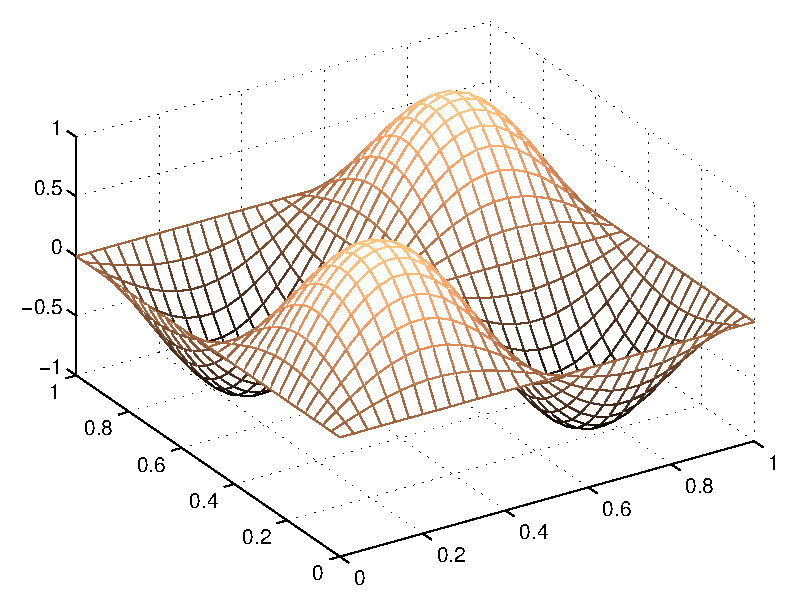
\includegraphics[width=0.4\textwidth]{figs/sine_wave_funct3}}
	}
	\subfigure[tilting slope]{
		\centering
		{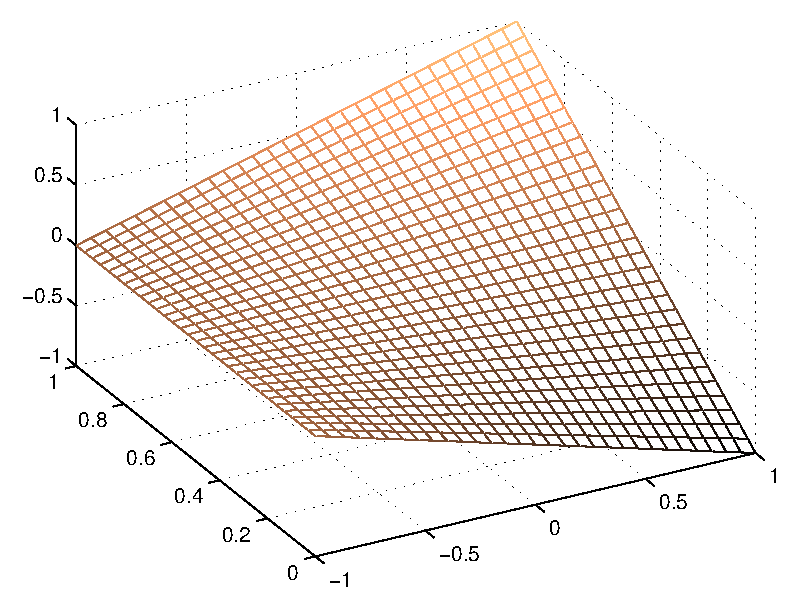
\includegraphics[width=0.4\textwidth]{figs/tilting_slope_funct3}}
	}
\caption{Two additively unfaithful functions. Relevant variables are
  zeroed out under an additive approximation because every ``slice''
  of the function integrates to zero.}
\vskip-10pt
\end{figure*}

In order to exploit additive models, it is important to understand when the
additive approximation accurately captures all of the relevant variables.
We call this property \textbf{additive faithfulness}. We first formalize the intuitive notion that a multivariate function $f$ \emph{depends on} a coordinate $x_k$.

\begin{definition}
  Let $F$ be a distribution on $\mathbf{C}=[0,1]^s$, and $f:\mathbf{C}\rightarrow \R$. 
  
We say that $f$ \textbf{depends on} coordinate $k$ if, for all $x_k \in [0,1]$, the set 
$\big\{ x'_k \in [0, 1] \,:\, f(x_k, \mathbf{x}_{-k}) = f(x'_k, \mathbf{x}_{-k}) 
\trm{ for almost all  $\mathbf{x}_{-k}$} \big\}$ 
has probability strictly less than 1.\\

Suppose we have the additive approximation:
\begin{equation}
f_k^*, \mu^* \coloneqq \argmin_{f_1,\ldots, f_s, \mu} \Bigl\{ 
             \E ( f(X) - \sum_{k=1}^s f_k(X_k) -\mu )^2 
         \,:\, \E f_k(X_k) = 0 \Bigr\}.
\end{equation}

We say that $f$ is \textbf{additively faithful} under $F$ in case $f^*_k = 0 \Rightarrow \trm{$f$ does not depend on coordinate $k$}$. 

\end{definition}
% We can define the support $\trm{supp}(f) \coloneqq \{ k \,:\,
% \trm{$k$ is relevant to $f$}\}$. Let $f^* = \sum_{k=1}^s$, then $f$
% is additively faith if $\trm{supp}(f) = \trm{supp}(f^*)$.

Additive faithfulness is an attractive property because it implies that, in the population setting, the additive approximation yields consistent variable selection. 

\subsection{Additive Faithfulness of Convex Functions}

Remarkably, under a general class of distributions which we characterize below, convex multivariate functions are additively faithful.

\begin{definition}
\label{defn:boundary-point}
Let $p(\mathbf{x})$ be a density supported on $[0,1]^s$, $p$ satisfies the \emph{boundary-points condition} if, for all $j$, and for all $\mathbf{x}_{-j}$:

\[
\frac{\partial p(\mathbf{x}_{-j} \given x_j)}{\partial x_j}  =  
\frac{\partial^2 p(\mathbf{x}_{-j} \given x_j)}{\partial x_j^2} = 0
\quad \trm{at } x_k = 0, x_k = 1
\]

\end{definition}



The boundary-points condition is a weak condition. For instance, it is satisfied when the density is flat at the boundary of support, more precisely, when the \emph{joint density} satisfies the properties that $\frac{\partial p(x_j,\mathbf{x}_{-j})}{\partial x_j} =  \frac{\partial^2 p(x_j, \mathbf{x}_{-j})}{\partial x_j^2} = 0$ at points $x_j = 0, x_j=1$. The boundary-points property is also trivially satisfied when $p$ is the density of any product distributions.

The following theorem is the main result of this section.

\begin{theorem}
\label{thm:convex_faithful}
Let $p$ be a positive density supported on $C=[0,1]^s$ that satisfies the boundary-points property (definition~\ref{defn:boundary-point}). If $f$ is convex and twice differentiable, then $f$ is \emph{additively faithful} under $p$.
\end{theorem}

% We give the full proof in Section~\ref{sec:faithful_proof} of the
% Appendix, but pause here to provide some intuition. 

We pause to give some intuition before we present the full proof: 
suppose the underlying distribution is a product distribution for a second, 
then we know from lemma~\ref{lem:general_int_reduction} that the
additive approximation zeroes out $k$ when, fixing $x_k$, every
``slice'' of $f$ integrates to zero. We prove
Theorem~\ref{thm:convex_faithful} by showing that ``slices'' of convex
functions that integrate to zero cannot be ``glued'' together while
still maintaining convexity.


\begin{proof} (of Theorem~\ref{thm:convex_faithful})\\
Fix $k$. Using the result of Lemma~\ref{lem:general_int_reduction}, we need only show that for all $x_k$, $ \E[ f(X) - \sum_{k'} f_{k'}(X_{k'}) \given x_k] - \E f(X) = 0 $ implies that $f$ does not depend on coordinate $k$.\\

Let us then use the shorthand notation that $r(\mathbf{x}_{-k}) = \sum_{k' \neq k} f_{k'}(x_{k'})$ and assume without loss of generality that $\mu = 0$. We then assume that for all $x_k$, 

\[
 \E[ f(X) - r(X_{-k})  \given x_k] \equiv 
 \int_{\mathbf{x}_{-k}}  p(\mathbf{x}_{-k} \given x_k ) 
 \big(f(\mathbf{x}) - r(\mathbf{x}_{-k}) \big) = 0
\]

We let $p'(\mathbf{x}_{-k} \given x_k)$ denote 
$\frac{\partial p(\mathbf{x}_{-k} \given x_k)}{\partial x_k}$ and 
$p''(\mathbf{x}_{-k} \given x_k)$ denote 
$\frac{\partial^2 p(\mathbf{x}_{-k} \given x_k)}{\partial x_k^2}$ and likewise for $f'(x_k, \mathbf{x}_{-k})$ and $f''(x_k, \mathbf{x}_{-k})$. We then differentiate under the integral, which is valid because all functions are bounded.

\begin{align}
& \int_{\mathbf{x}_{-k}} p'(\mathbf{x}_{-k} \given x_k) 
\big( f(\mathbf{x}) - r(\mathbf{x}_{-k}) \big) + 
p(\mathbf{x}_{-k} \given x_k) f'(x_k, \mathbf{x}_{-k}) d \mathbf{x}_{-k}  = 0 
\label{eqn:integral1a} \\
& \int_{\mathbf{x}_{-k}} p''(\mathbf{x}_{-k} \given x_k) 
\big( f(\mathbf{x}) - r(\mathbf{x}_{-k}) \big)  + 
2 p'(\mathbf{x}_{-k} \given x_k) f'(x_k, \mathbf{x}_{-k}) +
p(\mathbf{x}_{-k} \given x_k) f''(x_k, \mathbf{x}_{-k}) d\mathbf{x}_{-k}  = 0 
\end{align}

By the boundary-points condition, we have that $p''(\mathbf{x}_{-k} \given x_k)$ and $p'(\mathbf{x}_{-k} \given x_k)$ are zero at $x_k = x_k^0 \equiv 0$. The integral equations reduce to the following then:
\begin{align}
& \int_{\mathbf{x}_{-k}} p(\mathbf{x}_{-k} \given x^0_k) f'(x^0_k, \mathbf{x}_{-k}) d \mathbf{x}_{-k}= 0 \label{eqn:integral1b} \\
& \int_{\mathbf{x}_{-k}} p(\mathbf{x}_{-k} \given x^0_k) f''(x^0_k, \mathbf{x}_{-k}) d\mathbf{x}_{-k} = 0
\end{align}

Because $f$ is convex, $f(x_k, \mathbf{x}_{-k})$ must be a convex function of $x_k$ for all $\mathbf{x}_{-k}$. Therefore, for all $\mathbf{x}_{-k}$, $f''(x^0_k, \mathbf{x}_{-k}) \geq 0$. Since $p(\mathbf{x}_{-k} \given x^0_k) > 0$ by assumption that $p$ is a positive density, we have that $\forall \mathbf{x}_{-k}, f''(x^0_k, \mathbf{x}_{-k}) = 0$ necessarily.\\

The Hessian of $f$ at $(x^0_k, \mathbf{x}_{-k})$ then has a zero at the $k$-th main diagonal entry. A positive semidefinite matrix with a zero on the $k$-th main diagonal entry must have only zeros on the $k$-th row and column \footnote{ See proposition 7.1.10 of \citet{HJ90}}, which means that \emph{at all $\mathbf{x}_{-k}$, the gradient of $f'(x^0_k, \mathbf{x}_{-k})$ with respect to $\mathbf{x}_{-k}$ must be zero}.

Therefore, $f'(x_k^0, \mathbf{x}_{-k})$ must be constant for all $\mathbf{x}_{-k}$. By equation~\ref{eqn:integral1b}, we conclude then that $f'(x_k^0, \mathbf{x}_{-k}) = 0$ for all $\mathbf{x}_{-k}$. We can use the same reasoning for the case where $x_k = x_k^1$ and deduce that $f'(x^1_k, \mathbf{x}_{-k}) = 0$ for all $\mathbf{x}_{-k}$. \\

Because $f(x_k, \mathbf{x}_{-k})$ as a function of $x_k$ is convex, it must be that, for all $x_k \in (0,1)$ and for all $\mathbf{x}_{-k}$:
\[
0 = f'(x_k^0, \mathbf{x}_{-k}) \leq f'(x_k, \mathbf{x}_{-k}) \leq 
    f'(x_k^1, \mathbf{x}_{-k}) = 0
\]

Now we apply the first-order condition of convex functions to any two points $(x_k, \mathbf{x}_{-k})$ and $(x'_k, \mathbf{x}_{-k})$ where $x_k, x'_k \in [0,1]$:

\begin{align*}
\forall \mathbf{x}_{-k}, f(x'_k, \mathbf{x}_{-k}) & \leq f(x_k, \mathbf{x}_{-k}) 
  + f'(x_k, \mathbf{x}_{-k}) ( x'_k - x_k) \\ 
f(x'_k, \mathbf{x}_{-k}) &\leq f(x_k, \mathbf{x}_{-k}) \\
\forall \mathbf{x}_{-k}, f(x_k, \mathbf{x}_{-k}) & \leq f(x'_k, \mathbf{x}_{-k}) 
  + f'(x'_k, \mathbf{x}_{-k}) ( x_k - x'_k) \\ 
f(x_k, \mathbf{x}_{-k}) &\leq f(x'_k, \mathbf{x}_{-k})
\end{align*}

We thus have that $f(x_k, \mathbf{x}_{-k}) = f(x'_k, \mathbf{x}_{-k})$ for all $\mathbf{x}_{-k}$ and all pairs $x_k, x'_k \in (0,1)$. This proves that $f$ does not depend on $x_k$.
\end{proof}

Theorem~\ref{thm:convex_faithful} plays an important role in our
sparsistency analysis, where we show that the additive
approximation is variable selection consistent (or ``sparsistent''), even when the true function is not
additive.

\begin{remark}
  We assume twice differentiability in
  Theorems~\ref{thm:convex_faithful} to simplify the proof. 
  We believe
  this smoothness condition is not necessary because every non-smooth
  convex function can be approximated arbitrarily well by a smooth
  one.  
\end{remark}

\begin{remark} 
It is difficult to prove the opposite direction of additive faithfulness, that is, if $f$ does not depend on coordinate $k$, then $f_k^*$ will be zero in the additive approximation. Consider as a conceptual example a 3D distribution over $(X_1, X_2, X_3)$; suppose $X_1, X_2$ are independent, and $f$ is only a function of $X_1, X_2$. We can then let $X_3 = f(X_1, X_2) - f^*_1(X_1) - f^*_2(X_2)$, that is, we let $X_3$ exactly capture the additive approximation error, then the best additive approximation of $f$ would have a component $f^*_3(X_3) = X_3$ even though $f$ does not depend on $X_3$. 
\end{remark}



% \begin{remark}
% Without restrictions on the distribution, a convex
%   function may not be additively faithful. Intuitively, an arbitrarily shaped
%   density $p$
%   may ``undo'' the convexity of $f$ so that the product
%   $p(\mathbf{x}) \, f(\mathbf{x})$ resembles an egg carton or a
%   tilting slope.  With appropriate conditions on the density $p$,
%   however, it is possible to relax the independence assumption.  We leave this to
%   future work.
% \end{remark}


% DO NOT CHANGE; RefTex variables -minx
 
%%% Local Variables: ***
%%% mode:latex ***
%%% TeX-master: "paper.tex" ***
%%% End: ***


\def\C{\mathcal{C}}

\subsection{Estimation Procedure}
\label{sec:acdc}

Theorem~\ref{thm:acdc_faithful} naturally suggests 
a two-stage screening procedure for variable selection in the population setting. In the first stage, we fit a convex additive model. 
\begin{equation}
\label{eqn:scam2_pop}
f^*_1, ..., f^*_p = \argmin_{f_1,...,f_p \in \C^1_0} 
   \E \Big( f(X)  - \sum_{k=1}^p f_k(X_k) \Big)^2 
\end{equation}
where we denote $\C^1_0$ ($\mh{}\C^1_0$) as the set of one-dimensional convex (resp. concave) functions with population mean zero. In the second stage, for every variable marked as irrelevant in the first stage, we fit a univariate \emph{concave} function separately on the residual for that variable.
 for each $k$ such that $ f^*_k = 0$:
\begin{equation}
\label{eqn:dc2}
g^*_k = \argmin_{g_k \in \mh{}\C^1_0} 
   \E \Big( f(X) - \sum_{k'} f^*_{k'}(X_{k'}) 
    - g_k(X_{k})\Big)^2 
\end{equation}
We screen out $S^C$, any variable $k$ that is zero after the second stage, and output $S$.
\begin{equation}
\label{eqn:acdc_vars_pop}
S^c = \bigl\{k : f^*_k =
0 \; \mathrm{and}\; g^*_k =0\bigr\}.
\end{equation}

We refer to this procedure as AC/DC (additive
convex/decoupled concave). Theorem~\ref{thm:acdc_faithful} guarantees that the true set of relevant variables $S_0$ must be a subset of $S$.

% More precisely, given samples  
% $(\mathbf{x}_1, y_1), ..., (\mathbf{x}_n, y_n)$, 
% we perform the following steps.
% \begin{enumerate}
% \item {\it AC Stage}: Estimate an additive convex model
% \begin{equation}
% \label{eqn:scam}
% \hat{f}_1, ..., \hat{f}_p, \hat \mu  = \argmin_{f_1,...,f_p \in
%   \C^1_0, \,\mu\in\reals} 
%    \frac{1}{n} \sum_{i=1}^n \Big(y_i - \mu - \sum_{k=1}^p f_k(x_{ik}) \Big)^2 
%        + \lambda \sum_{k=1}^p \| f_k \|_\infty.
% \end{equation}
% \item {\it DC Stage}: For each $k$ such that $\| \hat{f}_k \|_\infty = 0$, estimate
%   a concave function on the residual:
% \begin{equation}
% \label{eqn:dc}
% \hat{g}_k = \argmin_{g_k \in \mh{}\C^1_0} 
%    \frac{1}{n} \sum_{i=1}^n \Big( y_i - \hat \mu - \sum_{k'} \hat{f}_{k'}(x_{ik'}) 
%     - g_k(x_{ik})\Big)^2 
%       + \lambda \| g_k \|_\infty.
% \end{equation}
% \item Output as the set of relevant variables
% $\hat S = \{ k \,:\, \| \hat{f}_k \|_\infty > 0 
%   \textrm{ or } \| \hat{g}_k \|_\infty > 0 \}$. 
% \end{enumerate}

%For identifiability, we impose the constraint $\sum_{i=1}^n f_k(x_{ik}) =
%0$ for each $k$.  
It is straightforward to construct a finite sample variable screening procedure, which we describe in Figure~\ref{fig:backfitting:algo}.
We use an $\ell_\infty/\ell_1$ penalty in equation~\eqref{eqn:scam2}
and an $\ell_\infty$ penalty in equation~\eqref{eqn:dc2} to encourage
sparsity.  Other penalties can also produce
sparse estimates, such as a penalty on the derivative of each of the
component functions.  The $\|\cdot\|_\infty$ norm is convenient for both
theoretical analysis and implementation.

The optimization in \eqref{eqn:scam2} appears to be infinite
dimensional, but it is equivalent to a finite dimensional quadratic
program.  In the following section, we give the details
of this optimization, and show how it can be reformulated
to be more computationally efficient.

%%For a simple proof of this fact, see \cite{Boyd04}, Section 6.5.5.
%%In more detail, we first set $\hat\mu = \frac{1}{n}\sum_{i=1}^n y_i$.  
%%For identifiability, we impose the constraint $\sum_{i=1}^n f_{ik} =
%%0$ for each $k$, where $f_{ik} = f_k(x_{ik})$ are the function values,
%%which are the program variables.  Then, we write the optimization as
%%\begin{align}
%%\label{eqn:scamqp}
%%\min_{f, \beta} \quad
%% &  \frac{1}{n} \sum_{i=1}^n \Big(y_i - \hat\mu - \sum_{k=1}^p f_{ik} \Big)^2 
%%       + \lambda \sum_{k=1}^p \| f_k \|_\infty \\
%%\nonumber
%%\text{such that} \quad & \textrm{for all $k=1,\ldots, p$:} \\
%% & \mathbf{1}^T f_k = 0, \; k=1,\ldots, p \\
%% & f_{i'k} \geq f_{ik} + \beta_{ik}(x_{i'k} - x_{ik}), \; \textrm{for
%%   all $i', i = 1,\ldots, n$}.
%%\end{align}
%%Likewise, the optimization in \eqref{eqn:dc} is implemented as
%%\begin{align}
%%\label{eqn:dcqp}
%%\min_{g_k, \gamma_k} \quad
%% &  \frac{1}{n} \sum_{i=1}^n \Big(y_i - \hat\mu - \sum_{k'=1}^p
%% f_{ik'} - g_{ik}\Big)^2 
%%       + \lambda \sum_{k=1}^p \| g_k \|_\infty \\
%%\nonumber
%%\text{such that} \quad &  \mathbf{1}^T g_k = 0, \\
%% & g_{i'k} \leq g_{ik} + \gamma_{ik}(x_{i'k} - x_{ik}), \; \textrm{for
%%   all $i', i = 1,\ldots, n$}.
%%\end{align}


\begin{figure}[t]
{\sc AC/DC Algorithm for Variable Selection in Convex Regression\hfill}
\vskip5pt
\begin{center}
\hrule
\vskip7pt
\normalsize
\begin{enumerate}
\item[] \textit{Input}:  $(\mathbf{x}_1, y_1), ..., (\mathbf{x}_n, y_n)$, regularization parameter $\lambda$.
\vskip5pt
\item[] \textit{AC Stage}:  Estimate a sparse additive convex model:
\begin{equation}
\label{eqn:scam2}
\hat{f}_1, ..., \hat{f}_p, \hat\mu = \argmin_{f_1,...,f_p \in \C^1_0} 
   \frac{1}{n} \sum_{i=1}^n \Big(y_i - \mu-\sum_{k=1}^p f_k(x_{ik}) \Big)^2 
       + \lambda \sum_{k=1}^p \| f_k \|_\infty
\end{equation}
\vskip5pt
\item[] \textit{DC Stage}:  Estimate concave functions
 for each $k$ such that $\| \hat{f}_k \|_\infty = 0$:
\begin{equation}
\label{eqn:dc2}
\hat{g}_k = \argmin_{g_k \in \mh{}\C^1_0} 
   \frac{1}{n} \sum_{i=1}^n \Big( y_i - \hat \mu - \sum_{k'} \hat{f}_{k'}(x_{ik'}) 
    - g_k(x_{ik})\Big)^2 
      + \lambda \| g_k \|_\infty
\end{equation}
\item[] \textit{Output}: Component functions $\{\hat f_k\}$ and 
relevant variables $\hat S$ where
\begin{equation}
\hat S^c = \bigl\{k : \| \hat{f}_k \| =
0 \; \mathrm{and}\; \|\hat{g}_k \|=0\bigr\}.
\end{equation}
\end{enumerate}
\vskip3pt
\hrule
\end{center}
\vskip0pt
\caption{The AC/DC algorithm for variable selection in convex
  regression.  The AC stage fits a sparse additive convex regression
  model, using a quadratic program that imposes an group sparsity
  penalty for each component function.  The DC stage fits
  decoupled concave functions on the residuals, for each 
  component that is zeroed out in the AC stage.}
\label{fig:backfitting:algo}
\end{figure}


% DO NOT CHANGE; RefTex variables -minx
 
%%% Local Variables: ***
%%% mode:latex ***
%%% TeX-master: "paper.tex" ***
%%% End: ***

\def\uds#1{#1}
\def\perm#1{\pi_k(#1)}

\section{Optimization}
\label{sec:optimization}

We now describe in detail the optimization algorithm for the additive
convex regression stage.  The second decoupled concave regression stage
follows a very similar procedure.

Let $\bds{x}_{i}\in\mathbb{R}^{p}$ be the covariate, let $y_{i}$ be
the response and let $\epsilon_{i}$ be the mean zero noise. The
regression function $f(\cdot)$ we estimate is the sum of
univariate functions $f_{k}(\cdot)$ in each variable dimension and a scalar
offset $\mu$.  We impose additional constraints that each
function $f_{k}(\cdot)$ is convex, which can be
represented by its supporting hyperplanes, i.e.,
\begin{equation}\label{hyper}
      f_{i'k} \geq f_{ik} + \beta_{ik}(x_{i'k}-x_{ik}) \quad
      \textrm{for all $i,i' = 1,\ldots, n$,}
\end{equation}
where $f_{ik}\coloneqq f_{k}(x_{ik})$ is the function value and $\beta_{ik}$ is a
subgradient at point $x_{ik}$. This ostensibly requires $O(n^2 p)$ constraints to
impose the supporting hyperplane constraints.
In fact, only $O(np)$
constraints suffice, since univariate convex functions are
characterized by the condition that the subgradient, which is a scalar, must
increase monotonically. This observation leads to the  optimization
\begin{equation}
\begin{split}
       \min_{f,\beta,\mu} & \;\; \frac{1}{2n}\sum_{i=1}^{n}
                     \Bigl( y_{i}-\mu - \sum_{k=1}^{p}f_{ik}\Bigr)^{2} 
                         + \lambda\sum_{k=1}^{p}\|f_k\|_{\infty} \\
       \textrm{subject to} &\;\; \textrm{for all $k=1,\ldots, p$:}\\
       & \;\; f_{\perm{i+1} k} = f_{\perm{i} k} +
       \beta_{\perm{i} k}(x_{\perm{i+1} k}-x_{\perm{i} k}),\;\textrm{for $i=1,\ldots, n-1$}\\
       & \;\; \sum_{i=1}^{n}f_{ik}=0,\\
       & \;\; \beta_{\perm{i+1} k} \geq \beta_{\perm{i} k}\;\textrm{for $i=1,\ldots, n-1$}.
\end{split}
\label{np}
\end{equation}
Here $f_k$ denotes the vector $f_k = (f_{1k}, f_{2_k}\ldots, f_{nk})^T\in\reals^n$
and $\{\perm{1},\perm{2},\ldots,\perm{n}\}$ are the indices in the sorted ordering
of the values of coordinate $k$:
\begin{equation}
x_{\perm{1} k} \leq{} x_{\perm{2} k} \leq \cdots \leq{} x_{\perm{n} k}.
\end{equation}


We can solve for $\mu$ explicitly as  
$\mu = \frac{1}{n} \sum_{i=1}^n y_i = \bar{y}$.  This follows from the
KKT conditions
and the constraints $\sum_i f_{ki} = 0$.
It is easy to verify that the constraints in \eqref{np} satisfy the
supporting hyperplane constraints, since
for all $j > i$
\begin{align*}
  f_{\perm{j}k}-f_{\perm{i}k}  & = \sum\limits_{t=i}^{j-1}(f_{\perm{t+1}k}-f_{\perm{t}k}) \\
   &= \sum\limits_{t=i}^{j-1}\beta_{\perm{t}k}(x_{\perm{t+1}k}-x_{\perm{t}k}) \\
   &\geq \beta_{\perm{i}k}\sum\limits_{t=i}^{j-1}(x_{\perm{t+1}k}-x_{\perm{t}k}) \\
  & = \beta_{\perm{i}k}(x_{\perm{j}k}-x_{\perm{i}k}) 
\end{align*}
and for all $j < i$
\begin{align*}
f_{k(j)}-f_{k(i)} & =
    \sum\limits_{t=j}^{i-1}(f_{k(t)}-f_{k(t+1)}) \\
     & = \sum\limits_{t=j}^{i-1}\beta_{k(t)}(x_{k(t)}-x_{k(t+1)}) \\
     &\geq \beta_{k(i)}\sum\limits_{t=j}^{i-1}(x_{k(t)}-x_{k(t+1)}) \\
     & = \beta_{k(i)}(x_{k(j)}-x_{k(i)}).
\end{align*}


%\begin{SCfigure}
%\label{fig:outer_approximation}
%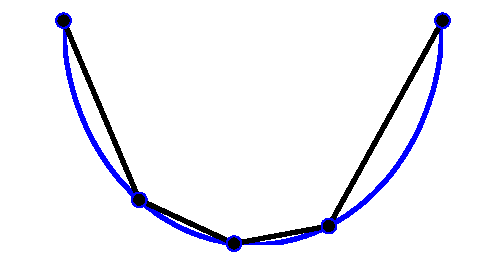
\includegraphics[width=0.3\textwidth]{figs/outer_approximation.pdf}
%\caption{With the 5 sample points $(X_i, h(X_i))$, the
%  black and the blue convex function represent equivalent fits. SCAM
%  chooses the inner piece-wise linear convex functions.}
%\end{SCfigure}

The sparse convex additive model optimization in \eqref{np} is a quadratic program with
$O(np)$ variables and $O(np)$ constraints. 
Directly applying a QP solver for $f$ and $\beta$
is computationally expensive for relatively large
$n$ and $p$. However, notice that variables in different feature
dimensions are only coupled in the squared error term
$(y_{i}-\mu - \sum_{k=1}^{p}f_{ik})^{2}$. Hence, we can apply the block
coordinate descent method, where in each step we solve the following
QP subproblem for $\{f_k, \beta_k\}$ with the
other variables fixed. In matrix notation, the optimization is
\begin{align}
\begin{split}
\min_{ f_k, \beta_k, \gamma_k} \;\;& \frac{1}{2n} \| \uds{r}_k - \uds{f}_k \|_2^2 
     + \lambda \gamma_k \label{opt:1d_compact} \\
 \textrm{such that } & P_k \uds{f}_k = \diag(P_k \bds{x}_k)  \uds{\beta}_k \\
   & D_k \uds{\beta}_k \leq 0 \\
   & -\gamma_k \mathbf{1}_n \leq \uds{f}_k \leq \gamma_k \mathbf{1}_n   \\
   & \mathbf{1}_n^\tran \uds{f}_k = 0 
\end{split}
\end{align}
where $\uds{\beta}_k \in \R^{n-1}$ is the vector $\uds{\beta}_k =
(\beta_{1k}, \ldots, \beta_{(n-1)k})^T$, and
$\uds{r}_{k} \in \R^n$ is the residual vector $\uds{r}_{k} = (y_i -
\hat\mu - \sum_{k' \neq k} f_{ik'})^T$.
In addition, 
$P_k \in \R^{(n-1) \times n}$ is a permutation matrix where the $i$-th
row  is all zeros except for the value $-1$ in position $\perm{i}$ and
the value $1$ in
position $\perm{i+1}$, and $D_k \in \R^{(n-2) \times (n-1)}$ is another
permutation matrix  where the $i$-th row is all zeros except for a
value $1$  in position $\perm{i}$ and a value $-1$ in position $\perm{i+1}$.  We denote by
$\diag( v )$ the diagonal matrix with diagonal entries $v$.
The extra variable $\gamma_{k}$ is introduced to impose the
regularization penalty involving the $\ell_{\infty}$ norm.  

% \begin{equation}
% \label{eqn:opt_1d}
% \begin{split}
%        \min_{\bds{h}_{k\cdot},\bds{\beta}_{k\cdot},\gamma_{k}} &
%              \ \frac{1}{2n}\sum_{i=1}^{n}\Bigl((Y_{i}-\bar{Y}
%                 -\sum_{r\neq{k}}f_{ri})-f_{ki}\Bigr)^{2} 
%                       + \lambda\gamma_{k} \\
%         \textrm{such that} & \ f_{k(i+1)} = f_{k(i)} + \beta_{k(i)}(x_{k(i+1)}-x_{k(i)}),\\
%         &\ \beta_{k(i+1)} \geq \beta_{k(i)}, \ -\gamma_{k}\leq f_{ki}\leq\gamma_{k}\\
%         &\  \sum_{i=1}^{n}f_{ki}=0, \ (\forall i).
% \end{split}
% \end{equation}

This QP
subproblem involves $O(n)$ variables, $O(n)$ constraints and a sparse
structure, which can be solved efficiently using optimization
packages. In our experiments we use {\sc mosek} (\href{http://www.mosek.com/}{www.mosek.com}).  We cycle through
all covariates $k$ from $1$ to $p$ multiple times until convergence.
Empirically, we observe that the algorithm converges in only a few
cycles. We also implemented an ADMM solver for \eqref{np}
\citep{Boyd:admm}, but found
that it is not as efficient as this blockwise QP solver.

After optimization, the function estimate for an input vector $\bds{x}$ is, according to \eqref{hyper},
\begin{equation}
\begin{split}
      \hat f(\bds{x}) & = \sum_{k=1}^{p} \hat f_k(x_{j})+ \hat \mu 
= \sum_{k=1}^{p}\max_{i} \Bigl\{\hat f_{ik}+ \hat \beta_{ik}(x_{k}-x_{ik})\Bigr\} +
      \hat \mu.
\end{split}
\end{equation} 

The univariate concave function estimation required in the DC stage is a straightforward
modification of optimization~\eqref{opt:1d_compact}. It is only
necessary to modify the linear inequality constraints so that the subgradients are
non-increasing: $\beta_{\perm{i+1}k} \leq \beta_{\perm{i}k}$.


\subsection{Alternative Formulation}
Optimization \eqref{np} can be reformulated in terms of the second
derivatives.  We exploit this form in our theoretical analysis. 

The alternative formulation replaces the order constraints
$\beta_{\perm{i+1}k} \geq \beta_{\perm{i}k}$ with positivity constraints, which
simplifies the analysis.  Define $d_{\perm{i}k}$ as the second
derivative: $d_{\perm{1}k} = \beta_{\perm{1}k}$, and $d_{\perm{i}k} = \beta_{\perm{i}k} -
\beta_{\perm{i-1}k}$ for $i > 1$. The convexity constraint is equivalent to the
constraint that $d_{\perm{i}k} \geq 0$ for all $i > 1$.

It is easy to verify that $\beta_{\perm{i}k} = \sum_{j \leq i} d_{\perm{j}k}$ and 
\begin{align*}
f_k(x_{\perm{i}k}) = & f_k(x_{\perm{i-1}k}) + \beta_{\perm{i-1}k}(x_{\perm{i}k} - x_{\perm{i-1}k}) \\
 =& f_k(x_{\perm{1}k}) + \sum_{j < i} \beta_{\perm{j}k} (x_{\perm{j}k} - x_{\perm{j-1}k}) \\
 =& f_k(x_{\perm{1}k}) + \sum_{j < i} \sum_{j' \leq j} d_{\perm{j'}k} (x_{\perm{j}k} - x_{\perm{j-1}k})\\
 =& f_k(x_{\perm{1}k}) + \sum_{j' < i} d_{\perm{j'}k} \sum_{i > j \geq j'} (x_{\perm{j}k} - x_{\perm{j-1}k}) \\
 =& f_k(x_{\perm{1}k}) + \sum_{j' < i} d_{\perm{j'}k} (x_{\perm{i}k} - x_{\perm{j'}k}).
\end{align*}
We can write this more compactly in matrix notation as
\begin{align}
\nonumber
\left[ \begin{array}{c}
f_k(x_{\perm{1}k}) \\
f_k(x_{\perm{2}k}) \\
\vdots \\
f_k(x_{\perm{n}k})
\end{array} \right] &=
\left[ \begin{array}{ccc}
    (x_{k1} - x_{\perm{1}k})_+ & \cdots & (x_{k1} - x_{\perm{n-1}k})_+ \\
    \cdots & & \\
    (x_{kn} - x_{\perm{1}k})_+ & \cdots & (x_{kn} - x_{\perm{n-1}k})_+ 
\end{array} \right]
\left[ \begin{array}{c}
    d_{\perm{1}k} \\
    \cdots \\
    d_{\perm{n-1}k}
\end{array} \right] + \mu_k \\[10pt]
& \equiv \Delta_k d_k + \mu_k
\end{align}
where $\Delta_k$ is a $n\times n-1$ matrix such that $\Delta_k(i,j) =
(x_{\perm{i}k} - x_{\perm{j}k})_+$, $d_k = (d_{\perm{1}k} ,\ldots,
d_{\perm{n-1}k})$, and $\mu_k = f_k(x_{\perm{1}k}) \mathbf{1}_n$.
Because $f_k$ has to be centered, $\mu_k = - \frac{1}{n}
\mathbf{1}_n^\tran \Delta_k d_k$, and therefore
\[
\Delta_k d_k + \mu_k \mathbf{1}_n = 
   \Delta_k d_k - \frac{1}{n} \mathbf{1}_n \mathbf{1}_n^\tran \Delta_k d_k = 
   \bar{\Delta}_k d_k 
\]
where $\bar{\Delta}_k \equiv \Delta_k - \frac{1}{n} \mathbf{1}_n \mathbf{1}_n^\tran \Delta_k$ is $\Delta_k$ with the mean of each column subtracted.

We can now reformulate \eqref{np} as an equivalent optimization program with only centering and positivity constraints:
\begin{align}
\min_{d_k}\;\; & \frac{1}{2n} 
       \Bigl\| Y - \sum_{k=1}^p 
              \bar{\Delta}_k d_k \Bigr\|_2^2 
               + \lambda_n \sum_{k=1}^p \|\bar{\Delta}_k d_k \|_\infty   
     \label{opt:alternate_opt} \\
\trm{such that}\;\;  & d_{\perm{2}k}, \ldots , d_{\perm{n-1}k} \geq 0  	
               \qquad \trm{(convexity).} \nonumber 
\end{align}

The decoupled concave postprocessing stage optimization is again
similar. Specifically, suppose $\hat{d}_k$ is the output of
optimization~\eqref{opt:alternate_opt}, and define the residual vector
\begin{equation}
\hat{r} = Y -
\sum_{k=1}^p \bar{\Delta}_k \hat{d}_k.
\label{eq:residual}
\end{equation}  
Then  for all $k$ such that $\hat{d}_k = 0$, the DC stage optimization is
formulated as
\begin{align}
  \min_{c_k}\;\; & 
      \frac{1}{2n} \Bigl \| \hat{r} - \Delta_k c_k \Bigr \|_2^2
      + \lambda_n \| \Delta_k c_k \|_\infty 
      \label{opt:alternate_opt_concave}\\
 \trm{such that }\;\; & c_{\perm{2}k}, \ldots, c_{\perm{n-1}k} \leq 0 \qquad \trm{(concavity).} \nonumber
\end{align}

We can use either the off-centered $\Delta_k$ matrix or the centered
$\bar{\Delta}_k$ matrix because the concave estimations are decoupled
and hence are not subject to non-identifiability under additive constants.

\begin{remark}
  In our analysis, we assume that an upper bound $B$ to
  $\| f^*_k \|_\infty$ is known, and that we constrain our estimate
  $\hat{f}$ to obey the same boundedness condition.  That is, for each
  $k$, we require that $\|\hat{f}_k\|_\infty \leq B$. This boundedness
  constraint can be easily added to our optimization program. In
  optimization~\eqref{opt:alternate_opt}, we can enforce the boundedness
  condition by adding $p$ constraints $\| \bar{\Delta}_k d_k
  \|_\infty \leq B$ for $k=1,\ldots,p$ (and similarly for
  optimization~\eqref{opt:alternate_opt_concave}). We emphasize that we
  use the boundedness constraint only in our theoretical analysis; 
  our experiments do not impose any such condition.
\end{remark}


% DO NOT CHANGE; RefTex variables -minx

%%% Local Variables: ***
%%% mode:latex ***
%%% TeX-master: "paper.tex" ***
%%% End: ***
\section{Analysis of Variable Selection Consistency}
\label{sec:finitesample}

We divide our analysis into two parts. We first establish a sufficient
deterministic condition for consistency of the sparsity pattern
selection procedure---a property sometimes called \textit{sparsistency}.
We then consider the
stochastic setting and argue that the deterministic conditions hold
with high probability. Note that in all of our results and analysis, we let $c,
C$ represent absolute constants; the actual values of $c,C$ may change from line to line.

\subsection{Deterministic Setting}

We construct an additive convex solution $\{\hat{d}_k\}_{k=1,\ldots,p}$
that is zero for $k \in S^c$, where $S$ is the set of relevant
variables, and show that it satisfies the KKT
conditions for optimality of optimization~\eqref{opt:alternate_opt}. We
define $\hat{d}_k$ for $k \in S$ to be a solution to the restricted
regression (defined below). We also show that $\hat{c}_k =
0$ satisfies the optimality condition of
optimization~\eqref{opt:alternate_opt_concave} for all $k \in S^c$.

\begin{definition}
\label{def:restricted_regression}
We define the \emph{restricted regression} problem 
\[
\min_{d_k} \frac{1}{n} \Big\| Y - \sum_{k \in S} \bar{\Delta}_k d_k \Big\|_2^2 + 
   \lambda_n \sum_{k \in S} \| \bar{\Delta}_k d_k \|_\infty \quad \trm{such that} \, d_{k,1}, \ldots, d_{k,n-1} \geq 0
\]
where we restrict the indices $k$ in
optimization \eqref{opt:alternate_opt} to lie in the set $S$ of true
relevant variables.
\end{definition}

\begin{theorem}[Deterministic setting]
\label{thm:deterministic}
Let $\{\hat{d}_k \}_{k \in S}$ be a minimizer of the restricted regression as defined above.
Let $\hat{r} \coloneqq Y - \sum_{k \in S} \bar{\Delta}_k \hat{d}_k$ be the restricted regression residual. 
Suppose for all $k\in S^c$, for all $i=1,\ldots,n$, $\lambda_n > | \frac{1}{2n}
\hat{r}^\tran \mathbf{1}_{(i:n)}|$ where $\mathbf{1}_{(i:n)}$ is 1 on
the coordinates of the 
$i$-th largest to the $n$-th largest entries of $X_k$ and 0
elsewhere.  Then the following two statements hold.
\begin{enumerate}
\item Let $\hat{d}_k = 0$ for $k \in S^c$.  Then
  \{$\hat{d}_k\}_{k=1,\ldots,p}$ is an optimal solution to
  optimization~\eqref{opt:alternate_opt}. Furthermore, any solution to
  the optimization program \eqref{opt:alternate_opt} must be zero on
  $S^c$.
\item For all $k \in S^c$, the solution $\hat{c}_k$ to optimization~\eqref{opt:alternate_opt_concave} must be zero.
\end{enumerate}

\end{theorem}

This result holds regardless of whether or not we impose the boundedness conditions in optimization~\eqref{opt:alternate_opt} and~\eqref{opt:alternate_opt_concave}.
The full proof of Theorem~\ref{thm:deterministic} is in Section~\ref{sec:deterministic_proof} of the Appendix.

Theorem~\ref{thm:deterministic} allows us to separately analyze the false negative
rates and false positive rates. To control false positives,
we analyze the condition on $\lambda_n$ for $k \in S^c$. To control
false negatives, we analyze the restricted regression. 

The proof of Theorem~\ref{thm:deterministic} analyses the KKT
conditions of optimization~\eqref{opt:alternate_opt}.  This parallels
the now standard \emph{primal-dual witness}
technique~\citep{wainwright2009sharp}. However, we cannot derive analogous
\emph{mutual incoherence} conditions because the estimation is
nonparametric---even the low dimensional restricted regression has
$s(n-1)$ variables. The details of the proof are given in
Section~\ref{sec:deterministic_proof} of the Appendix.

\subsection{Probabilistic Setting}

In the probabilistic setting we treat the covariates as random.  We
adopt the following standard setup:

\begin{enumerate}
\item The data $X^{(1)},\ldots, X^{(n)} \sim F$ are iid from
a distribution $F$ that is supported and strictly positive on $\mathcal{X}=[-b,b]^p$. 
\item The response is $Y = f_0(X) + W$ where $W$ is
  independent, zero-mean noise; thus $Y^{(i)} = f_0(X^{(i)}) + W^{(i)}$.
\item The regression function $f_0$ satisfies
$f_0(X) = f_0(X_{S_0})$, where $S_0 = \{1,\ldots,s_0\}$ is the set of
relevant variables.
\end{enumerate}


Let $\mathcal{C}^1$ denote the set of univariate convex functions
supported on $[-b,b]$, 
and let  $\mathcal{C}_1^{p}$ denote the set of convex additive functions
$\mathcal{C}_1^p \equiv \{ f \,:\, f = \sum_{k=1}^p f_k, \,
   f_k \in \mathcal{C}^1 \} $.  
Let $f^*(x) = \sum_{k=1}^p f^*_k(x_k)$ be the population risk
minimizer in $\mathcal{C}_1^p$, 
\begin{equation}
f^* \equiv \arg\min_{f \in \mathcal{C}_1^p} \E\big(f_0(X) - f^*(X)
\big)^2.
\end{equation}
Similarly, we define $\mh \mathcal{C}^1$ as the set of univariate concave functions supported on $[-b, b]$ and define
\begin{equation}
g^*_k = \arg\min_{g_k \in \mh \mathcal{C}^1} \E \big( f_0(X) - f^*(X)
- g_k(X_k) \big)^2.
\end{equation}
We let $S = \{ k = 1,\ldots,p \,:\, f^*_k \neq 0 \trm{ or } g^*_k \neq 0\}$. By additive faithfulness (Theorem~\ref{thm:acdc_faithful}), it must be that $S_0 \subset S$. 


Each of our theorems will use a subset of the following assumptions:
\begin{packed_enum}
\item[A1:] $X_S, X_{S^c}$ are independent. 
\item[A2:] $f_0$ is convex and twice-differentiable. 
\item[A3:] $\|f_0\|_\infty \leq sB$ and $\| f^*_k \|_\infty \leq B$ for all $k$.
\item[A4:] $W$ is mean-zero sub-Gaussian, independent of $X$, with scale $\sigma$; i.e., for all $t \in \R$, $\E e^{t \epsilon} \leq e^{\sigma^2 t^2 / 2}$.
\end{packed_enum}
By assumption A1, $f^*_k$ is must be zero for $k\notin S$.
We define $\alpha_f, \alpha_g$ as a measure of the signal strength of the weakest variable:
\begin{align*}
\alpha_f &= \inf_{f \in \mathcal{C}_1^p \,:\, \exists k ,\, f^*_k \neq 0 \,\wedge\, f_k = 0} 
       \Big\{ \mathbb{E} \big( f_0(X) - f(X) \big)^2 - 
        \mathbb{E} \big( f_0(X) - f^*(X) \big)^2  \Big\}\\
\alpha_g &=   \min_{k \in S \,:\, g^*_k \neq 0}
      \Big\{ \mathbb{E} \big( f_0(X) - f^*(X) \big)^2 - 
    \mathbb{E} \big( f_0(X) - f^*(X) - g^*_k(X_k) \big)^2 \Big\}
\end{align*}
These play the role of the absolute value of the smallest nonzero
coefficient in the true linear model in lasso theory.  Intuitively, if
$\alpha_f$ is small, then it is easier to make a false omission in the
additive convex stage of the procedure. If $\alpha_g$ is small, then
it is easier to make a false omission in the decoupled concave stage
of the procedure.

\begin{remark}
  We make strong assumptions on the covariates in A1 in order to make
  very weak assumptions on the true regression function $f_0$ in
  A2. In particular, we do not assume that $f_0$ is additive. 
  %Strong assumptions on the covariates are not uncommon in nonparametric
  %variable selection analysis~\cite{lafferty2008rodeo}. 
  %[TODO: refer to correlated design experiment].
\end{remark}


\begin{theorem}[Controlling false positives]
\label{thm:false_positive}
Suppose assumptions A1-A4 hold. Define $\tilde{\sigma} \equiv \max(\sigma, B)$,
and suppose 
\begin{equation}
\lambda_n \geq 8 s_0 \tilde{\sigma}  \sqrt{ \frac{\log^2 np}{n}}.
\end{equation}  
Then with probability at least $ 1 - \frac{12}{np}$, for all $k \in
S^c$, and for all $i'=1,\ldots, n$,
\begin{equation}
\Big| \frac{1}{2n}\hat{r}^\tran \mathbf{1}_{(i':n)_k} \Big| < \lambda_n
\end{equation}
and for all $k \in S^c$, both the AC solution $\hat{f}_k$ from optimization~\eqref{opt:alternate_opt} and the DC solution $\hat{g}_k$ from optimization~\eqref{opt:alternate_opt_concave} are zero. 
\end{theorem}

The proof of Theorem~\ref{thm:false_positive} exploits independence of
$\hat{r}$ and $X_k$ from A1; when $\hat{r}$ and $X_k$ are independent,
$\hat{r}^\tran \mathbf{1}_{(i':n)}$ is the sum of $n - i' +1$ random
coordinates of $\hat{r}$.  We can then use concentration of
measure results for sampling without replacement to argue that $|
\frac{1}{n} \hat{r}^\tran\mathbf{1}_{(i':n)}|$ is small with high
probability. The full proof of Theorem~\ref{thm:false_positive} is in
Section~\ref{sec:false_positive_proof} of the Appendix.

\begin{theorem} (Controlling false negatives) 
\label{thm:false_negative}
Suppose assumptions A1-A4 hold. Let $\hat{f}$ be any AC solution to the restricted regression with $B$-boundedness constraint and let $\hat{g}_k$'s be any DC solution to the restricted regression with $B$-boundedness constraint. Let $\tilde{\sigma}$ denote $\max(\sigma, B)$.

Suppose $\lambda \leq 9 s \tilde{\sigma} \sqrt{\frac{1}{n} \log^2 np}$ and $n$ is large enough such that $\frac{n^{4/5}}{\log np} \geq B^4 \tilde{\sigma}^2 s^5$. 

Suppose 
$\alpha_f/\tilde{\sigma} \geq c B^2 \sqrt{\frac{s^5}{n^{4/5}} \log^2 np}$ and $\alpha_g^2/\tilde{\sigma} \geq c B^2 \sqrt{\frac{s^5}{n^{4/5}} \log^2 np}$ where $c$ is a constant.

Then, with probability at least $1 - \frac{C}{n}$ for some constant $C$, we have that for all $k \in S$, $\hat{f}_k \neq 0$ or $\hat{g}_k \neq 0$. 

\end{theorem}

This is a finite sample version of
Theorem~\ref{thm:convex_faithful}. We need stronger assumptions in
Theorem~\ref{thm:false_negative} to use our additive faithfulness
result, Theorem~\ref{thm:convex_faithful}. We also include an extra
boundedness constraint so that we can use recent bracketing number
results \cite{kim2014global}.

Combining Theorem~\ref{thm:false_positive} and
~\ref{thm:false_negative} 
we have the following result.
\begin{corollary}
Suppose assumptions A1-A4 hold. Let $\hat{f}$ be any AC solution and $\hat{g}_k$'s be any DC solution, both with $B$-boundedness constraints, both with 
$\lambda = \Theta\big( s \tilde{\sigma} \sqrt{\frac{1}{n} \log^2 np} \big) $. Let $\tilde{\sigma} \equiv \max(\sigma, B)$.


Suppose 
$\alpha_f/\tilde{\sigma} \geq c B^2 \sqrt{\frac{s^5}{n^{4/5}} \log^2 np}$ and $\alpha_g^2/\tilde{\sigma} \geq c B^4 \sqrt{\frac{s^5}{n^{4/5}} \log^2 np}$.

Then, for all large enough $n$ such that $\frac{n^{4/5}}{\log^2 np} \geq B^4 \tilde{\sigma}^2 s^5$, we have that with probability at least $1-\frac{C}{n}$:
\begin{align*}
\hat{f}_k \neq 0 \trm{ or } \hat{g}_k \neq 0 &\trm{ for all } k \in S\\
\hat{f}_k = 0 \trm{ and } \hat{g}_k = 0 & \trm{ for all } k \notin S
\end{align*}

where $c,C$ are constants.

\end{corollary}
The above corollary implies that sparsistency is achievable at the same exponential scaling of the ambient dimension $p = O(\exp(n^c)), c<1$ rate as parametric models. The cost of nonparametric modeling is reflected in the scaling with respect to $s$, which can only scale at $o(n^{4/25})$.

\begin{remark}
\citet{dalalyan:12} have shown that under tradtional smoothness constraints, even with a product distribution, variable selection is achievable only if $n > O(e^s)$. It is interesting to observe that because of additive faithfulness, the convexity assumption enables a much better scaling of $n = O(\textrm{poly}(s))$, demonstrating that geometric constraints can be quite different from the previously studied smoothness conditions.
\end{remark}

%\textbf{Comparison with Related Work.} 


% DO NOT CHANGE; RefTex variables -minx
 
%%% Local Variables: ***
%%% mode:latex ***
%%% TeX-master: "paper.tex" ***
%%% End: ***

\def\x{x}
\def\Q{Q}
\def\bds#1{#1}
\def\tts#1{\texttt{\small #1}}

\section{Experiments}
\label{sec:thesims}

We perform both synthetic and real data experiments.

\subsection{Simulations}
We first illustrate our methods using a simulation of the model
\begin{equation}\nonumber
         Y_i = f_o(\x_{iS}) + \epsilon_i \quad (i=1,2,\ldots,n).
\end{equation}
Here $\x_{i}$ denotes data sample $i$ drawn from some distribution $P$. $f_0$ is the true regression function. $\x_{iS}$ is a subset of $\x_i$ with dimension $|S|=s$, where $S$
represents the set of relevant variables, and 
$\epsilon_i$ is additive noise drawn from $\mathcal{N}(0,\sigma)$. For 
all simulations, we set $\sigma$ such that the signal-to-noise ratio(SNR, $\frac{\trm{std}(Y)}{\sigma}$) is 5. Also, for all simulations except the sixth, we choose the set of relevant variables $S$ uniformly at random among all variables $\{1,...,p\}$.

We study both the independent case where $P = N(0, I_p)$ and the correlated case where $P$ is a correlated Gaussian Copula modified slightly to satisfy the boundary flatness condition. We measure the probability of exact selection in the independent case and the probability of screening in the correlated case. We also study both cases where the regression function is parametric (quadratic) and cases where the regression function is nonparametric (softmax of linear forms). In all our experiments, we mark a variable as selected if either the AC estimate $\| \hat{f}_j \|_\infty$ or the DC estimate $\| \hat{g}_k \|_\infty$ is larger than $10^{-6}$. We set $\lambda = 0.5 \sqrt{\frac{\log^2 np}{n}}$ for all the simulations.

For the first three simulations, we will use the quadratic form as our true regression function.
\[
f_0(x_{iS}) = x_{iS}^\tran \Q x_{iS}
\]

The matrix $\Q$ is a symmetric positive definite matrix of dimension $s \times{} s$. 
Note that if $\Q$ is diagonal, then the true function is convex
additive; 
otherwise the true function is convex but not additive.

In the \textbf{first simulation} (Figure~\ref{Support}a), we vary the ambient dimension $p$. We set $Q$ as one on the diagonal and $1/2$ on the off-diagonal with $0.5$ probability, set $s=5$, and $p=64,128,256$ and $512$. We draw $X \sim N(0, I_p)$.
For each $(n,p)$ combination, we generate $100$ independent trials. 
In Figure~\ref{Support}(a), we plot the probability of exact
support recovery. We observe that the algorithm performs consistent variable selection even if the dimensionality is large. To give the reader a
sense of the running speed, for a 
data set with $n=1000$ and $p=512$, the code runs in roughly two 
minutes on a machine with 2.3 GHz Intel Core i5 CPU and 4 GB memory. 


In the \textbf{second simulation} (Figure~\ref{Support}b,c), we vary the sparsity of the $Q$ matrix, that is, we vary the extent to which the true function is non-additive. We generate four $\Q$ matrices
plotted in Figure \ref{Support}(c), where the diagonal elements are all one and
the off-diagonal elements are $\frac{1}{2}$ with probability $\alpha$
($\alpha=0,0.2,0.5,1$ for the four cases). We show the 4 $\Q$ matrices we used in Figure~\ref{Support}(c).
We fix $p=128$, $s=5$, and $X \sim N(0,I_p)$.  We again run the AC/DC optimization on $100$
independent trials and plot the probability of exact recovery
in Figure \ref{Support}(b). The results demonstrate that AC/DC performs
consistent variable selection even if the true function is not additive (but
still convex). 

In the third, fourth, and fifth simulation, we use a correlated design. We generate $X$ from a non-Gaussian boundary flat distribution with covariance $\Sigma$. The distribution we used is a mixture of a uniform distribution and a Gaussian Copula.
\[
X \sim \gamma U([-2, 2]^p) + (1-\gamma) \trm{Copula}(0, \Sigma, F)
\]
The Gaussian Copula is a way to customize the marginal distributions of a Gaussian random variable while maintaining the same covariance. Gaussian Copula results when one applies a monotone transformation $F^{-1} \Phi$ onto each of the variables of a Gaussian random vector where $\Phi$ is the normal CDF and $F$ is the CDF of the new marginal distribution. In all our experiments, we set $\gamma = 0.05$ and set the marginal CDF $F$ so that marginal density of the Copula is bimodal and supported on $[-1.8, 1.8]$. The resulting marginal density of the mixture is shown in Figure~\ref{fig:copula_marginal}. Notice that boundary flatness holds because the distribution is uniform in the boundary area $[-2,2]^p \backslash [-1.8, 1.8]^p$.

\begin{figure*}
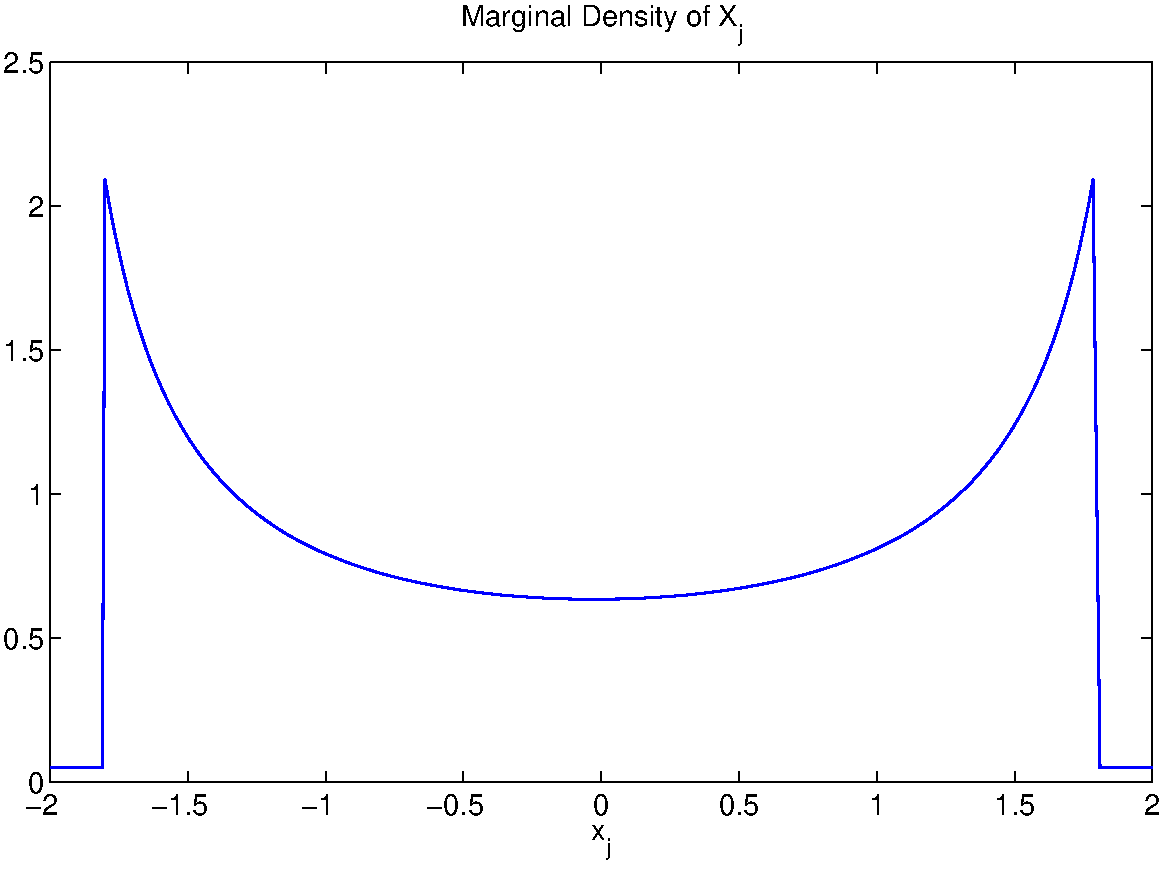
\includegraphics[width=.4\textwidth]{figs/copula_marginal}
\caption{Marginal density of the Gaussian Copula and Uniform Mixture}
\label{fig:copula_marginal}
\end{figure*}

In the \textbf{third simulation} (Figure~\ref{Support}d,e), we use the non-Gaussian distribution described above and set the covariance $\Sigma_{ij}=\nu^{|i-j|}$ for $\nu = 0, 0.2, 0.5, 0.9$. We use the non-additive $\Q$, same as in the first experiment, with $\alpha=0.5$ and fix $p=128, s=5$. We measure success not through exact recovery but through faithful recovery. We say that a trial is a successful if (1) all relevant variables were recovered and (2) fewer than $20$ variables were marked as relevant overall (true sparsisty $s=5$). We use the same $\lambda$ as before. The probabilities of success are computed from 40 independent trials and plotted against various values of $\nu$ in Figure~\ref{Support}(d). Additionally, for $\nu = 0.5$, we show the number of selected variables versus the sample size as a box-and-whisker plot in Figure~\ref{Support}(e). As seen, for small to moderate correlations, AC/DC can successfully recover the relevant variables with only a small number of false positives. 

In the fourth and fifth simulation, we use a softmax function as the ground truth
\begin{align}
f_0(x_{iS}) = \log \left( \sum_{k=1}^K \exp( \beta_k^\tran x_{iS} ) \right) - \mu
\end{align}
We generate random unit vectors as $\{\beta_k \in \R^s\}_{k=1,...,K}$ and choose $\mu$ so that $f_0$ has mean-zero. We set $K = 7$ for all the experiments. 

For the \textbf{fourth simulation} (Figure~\ref{Support}f,g), we let $f_0$ be the softmax function and let $X$ be drawn from the boundary flat mixture distribution described earlier with the Toeplitz covariance $\Sigma_{ij}=\nu^{|i-j|}$ for $\nu = 0.5$. We set $s=5$ and vary $p=128,256,512$. We use the same faithful recovery criteria as the third simulation and plot the probability of faithful recovery against the number of samples in Figure~\ref{Support}(f). The probabilities are computed over 30 independent trials. Also, for $p=256$, we show the number of selected variables versus the sample size as a box-and-whisker plot in Figure~\ref{Support}(g). The softmax function is more challenging to estimate than the quadratic function; the softmax function requires about $n > 1500$ to achieve the same success probability as the quadratic function with $n=1000$. Regardless, we see that increasing the ambient dimension $p$ does not signficantly affect the recovery probability.

%For the \textbf{fifth experiment} (Figure~\ref{Support}h), we vary the true sparsity level $s$. We let $f_0$ be the softmax function, $X \sim N(0, I)$, and set $p=128$. We compute the probability of exact recovery over 40 independent trials and plot the results in Figure~\ref{Support}(h).  

For the \textbf{fifth simulation} (Figure~\ref{fig:ac_v_dc}), we compare the variables selected via the AC stage and the variables selected via the DC stage. We use the softmax regression function and $X$ drawn from the boundary flat mixture distribution with a Toeplitz covariance and correlation level $\nu = -0.7$. We set $s=5, n=500, p=128$. We perform 30 independent trials and plot the frequency of variable selection in Figure~\ref{fig:ac_v_dc}. The true variables are $X_j$ for $j=5,6,7,8,9,10$. We plot the frequency of selection among only the first 20 variables, that is, $X_j$ for $j=1,...,20$. We do not plot selection frequencies for variables 21 to 128 because they are almost never selected by either AC or DC. As can be seen, the DC stage is slightly helpful in recovering the true variables but its effect is not significant. We thus believe that the DC stage, though important in theory, is not as important in practice; it may be omitted without significant detriment to the overall result. 

\begin{figure*}[!t]
\begin{center}
\begin{tabular}{cc}
%\hskip-10pt
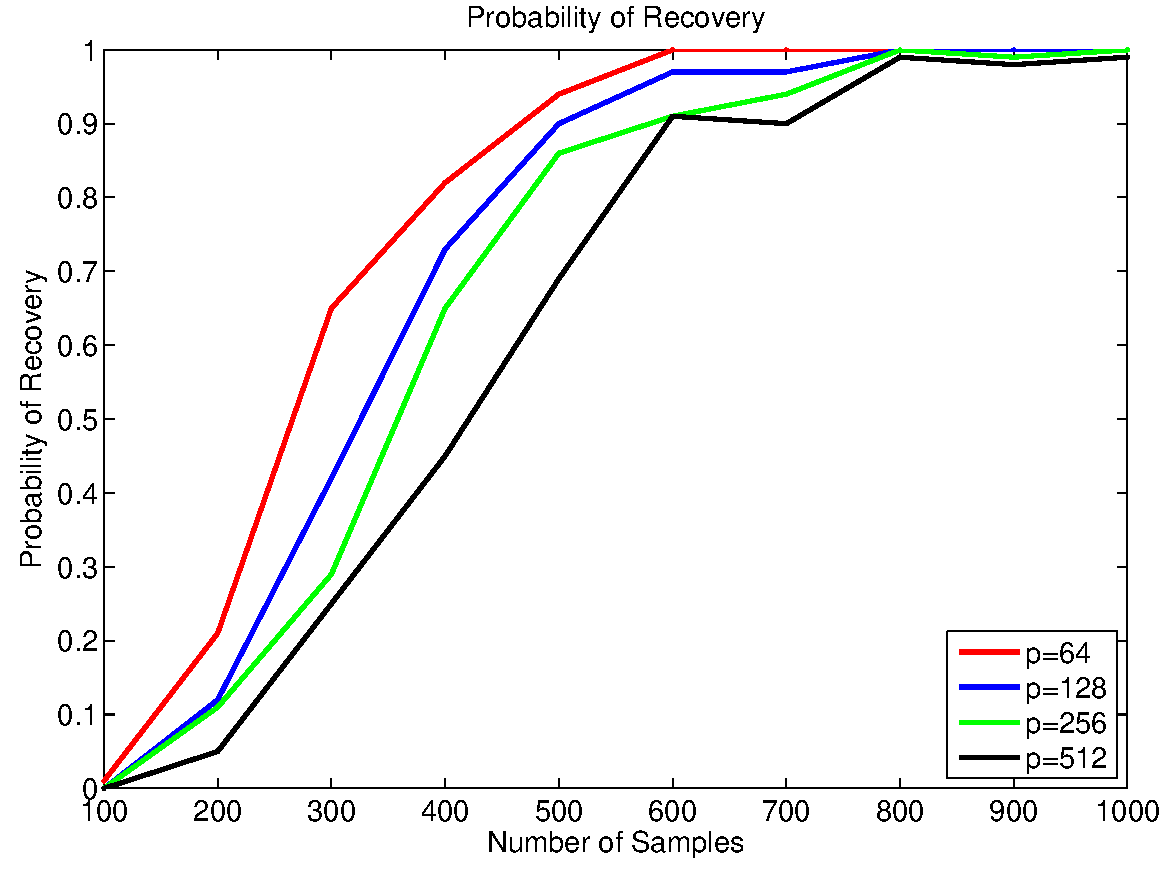
\includegraphics[width=.42\textwidth]{figs/CurveT} &
%\hskip-10pt
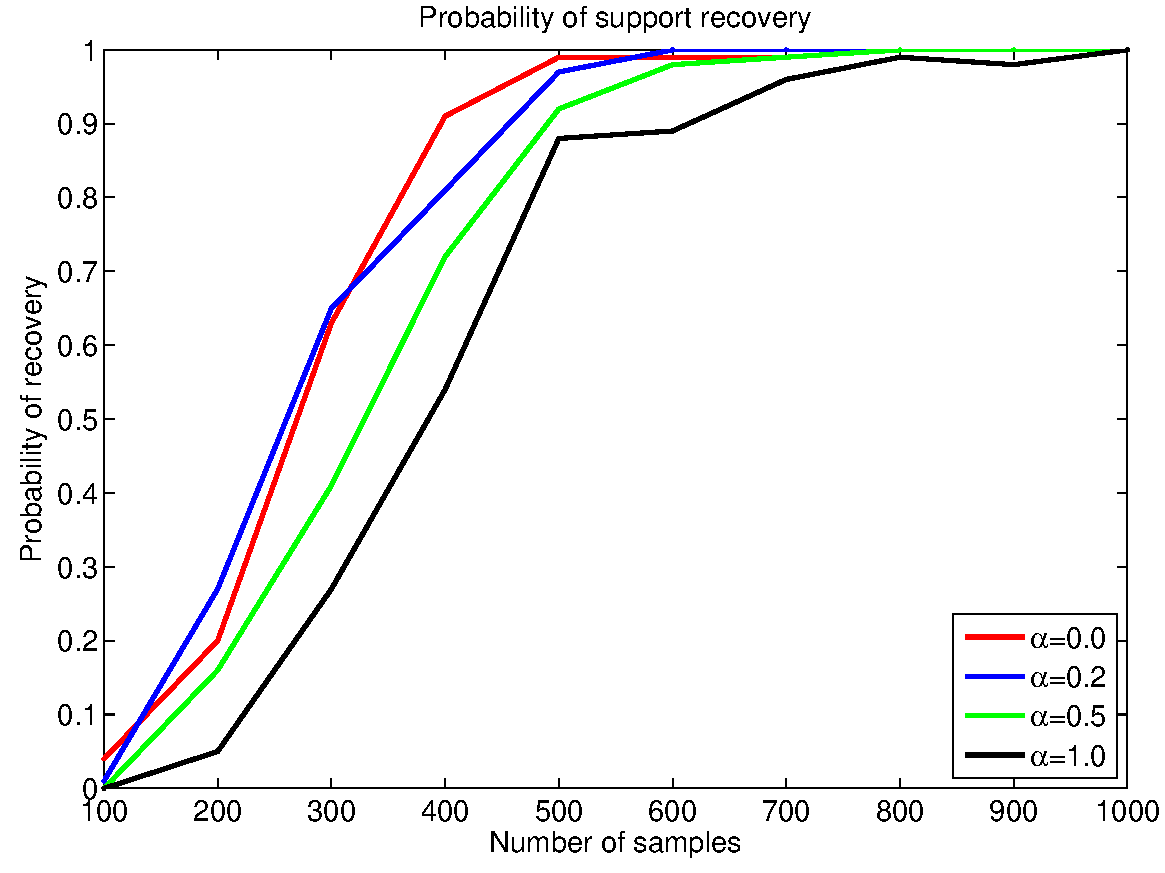
\includegraphics[width=.42\textwidth]{figs/CurveR} \\
(a) quadratic $f_0$, independent $X$, varying $p$  & (b) quadratic $f_0$, independent $X$, varying $\Q$ \\
%\hskip-10pt
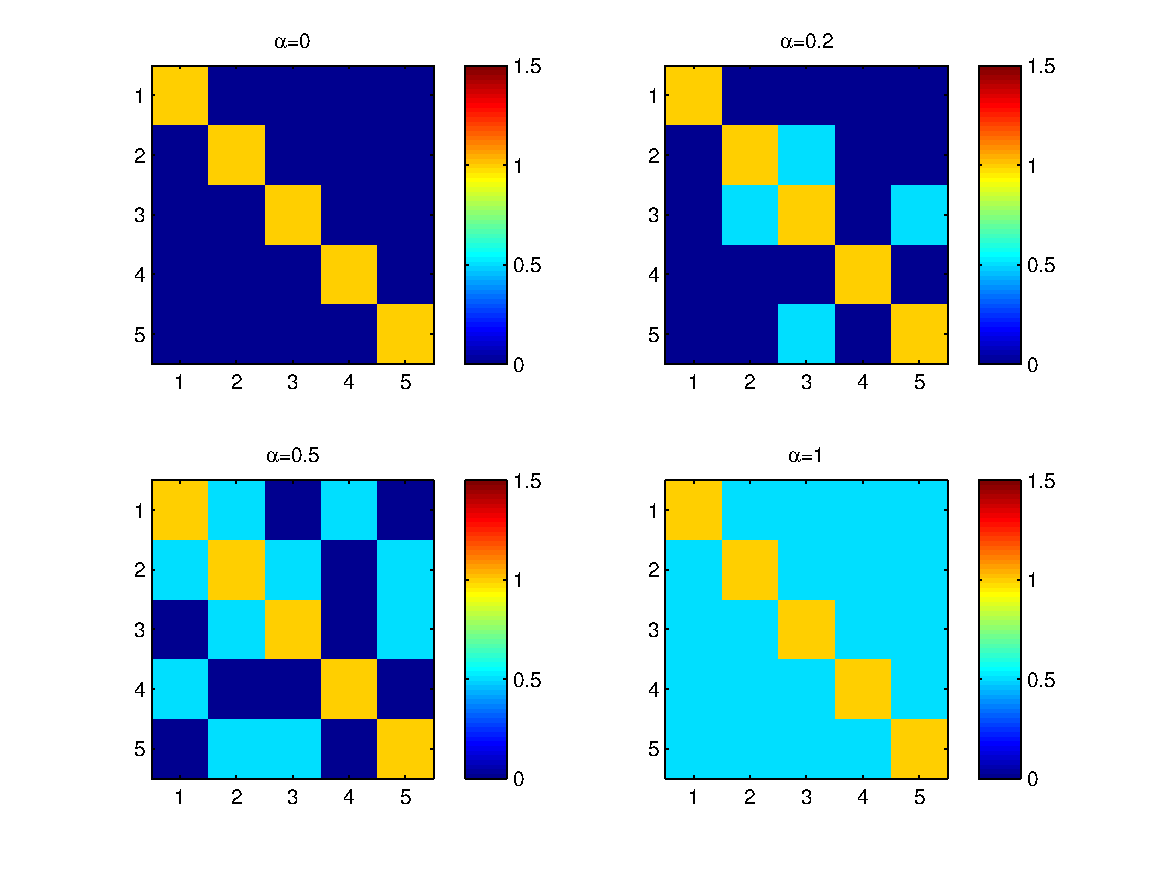
\includegraphics[width=.42\textwidth]{figs/Q} &
%\hskip-10pt
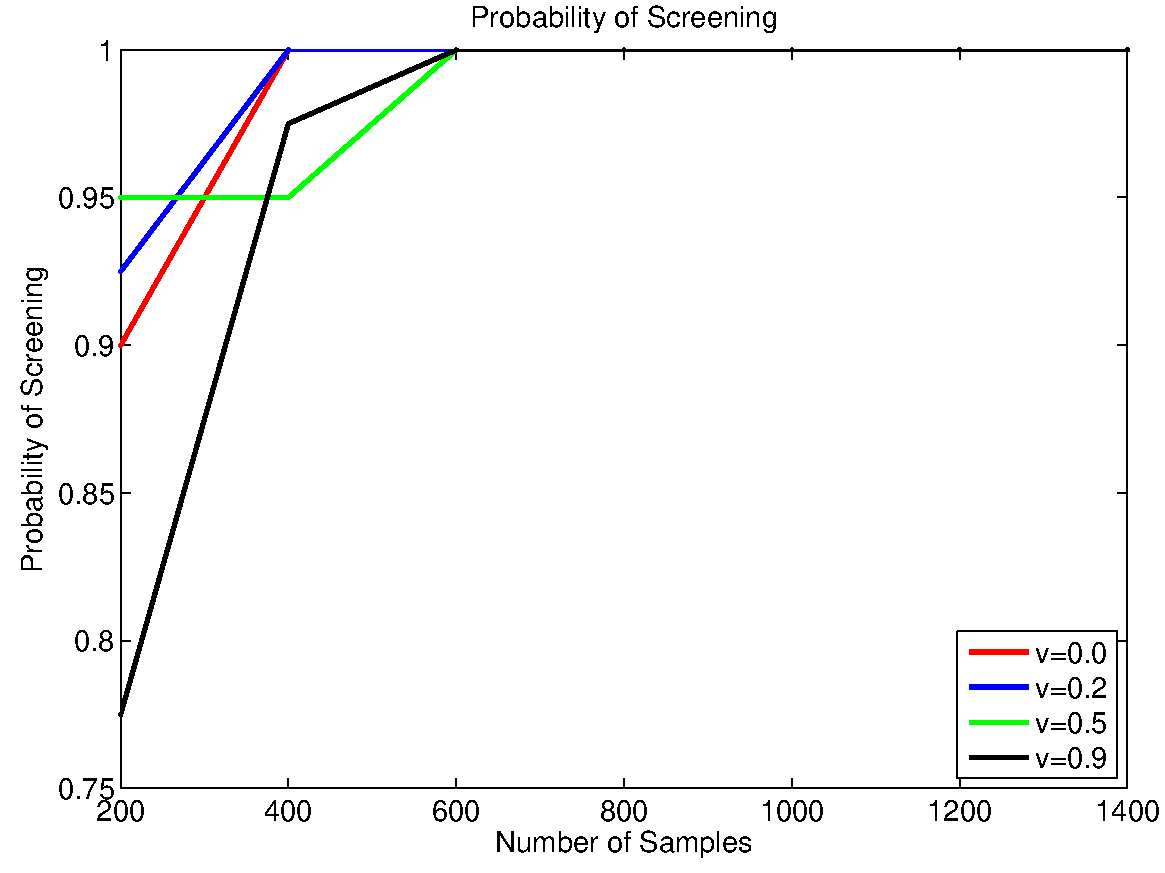
\includegraphics[width=.42\textwidth]{figs/CurveC}  \\
(c) four $\Q$ matrices used in (b) & (d) quadratic $f_0$, correlated $X$, varying correlation $\nu$ \\
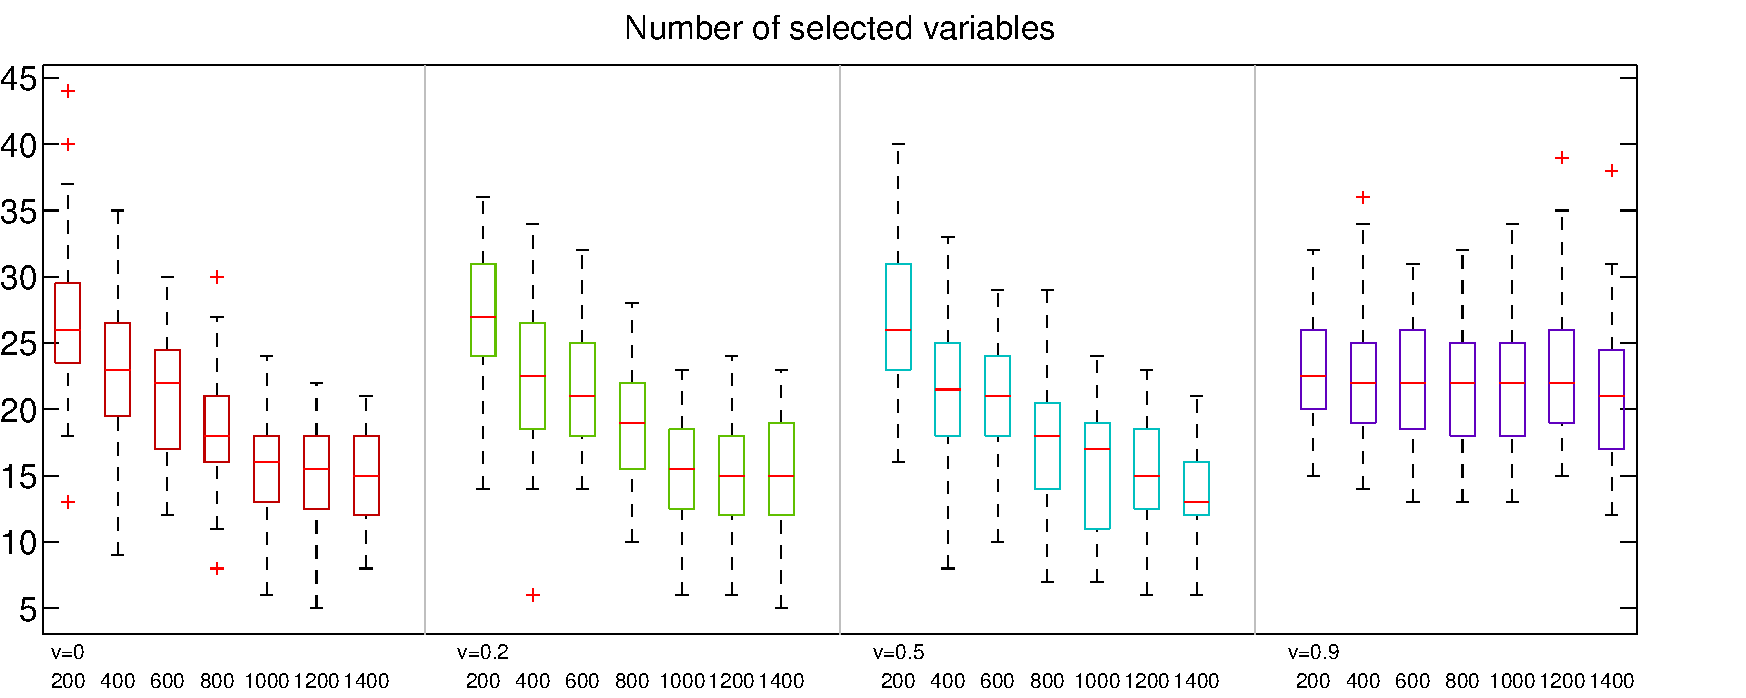
\includegraphics[width=.42\textwidth]{figs/C_support_box} & 
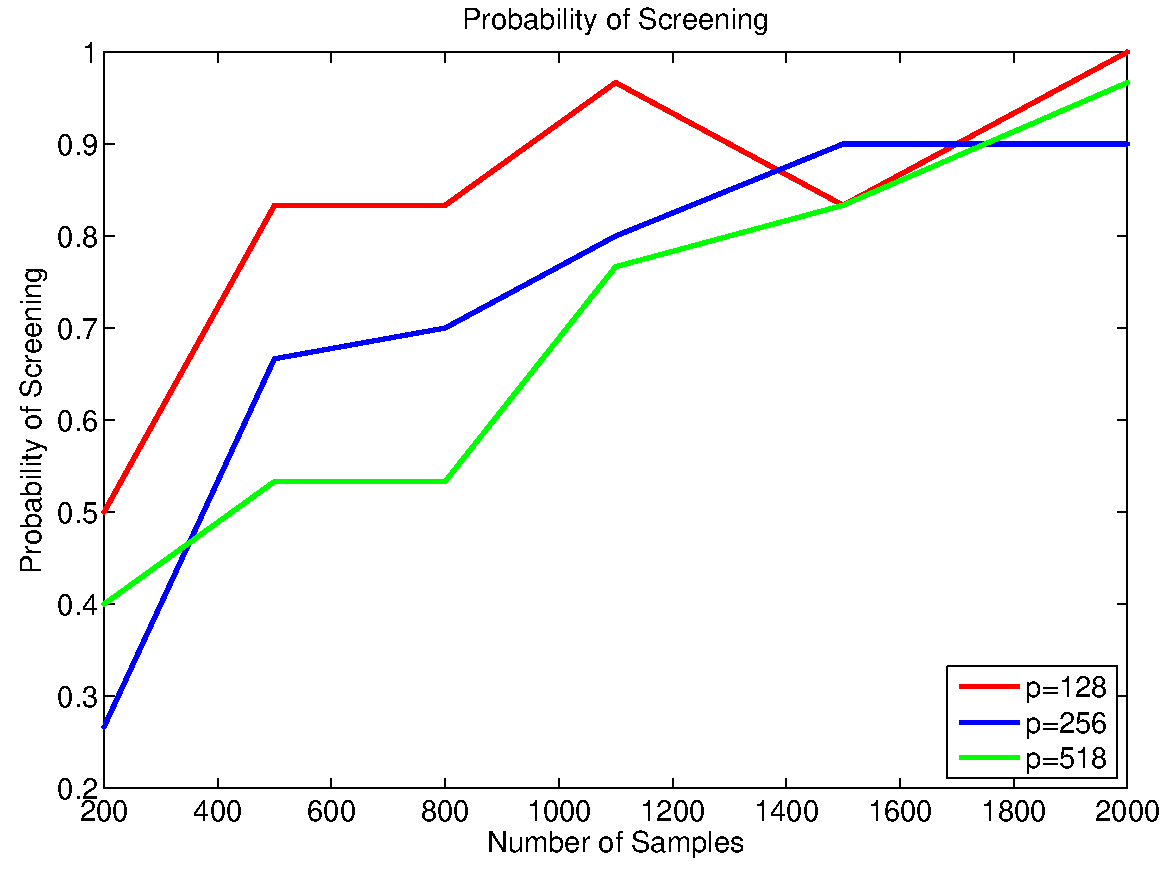
\includegraphics[width=.42\textwidth]{figs/CurveS}\\
(e) recovered support size for $\nu=0.5$ in (d) & (f) softmax $f_0$, correlated $X$, varying $p$ \\
%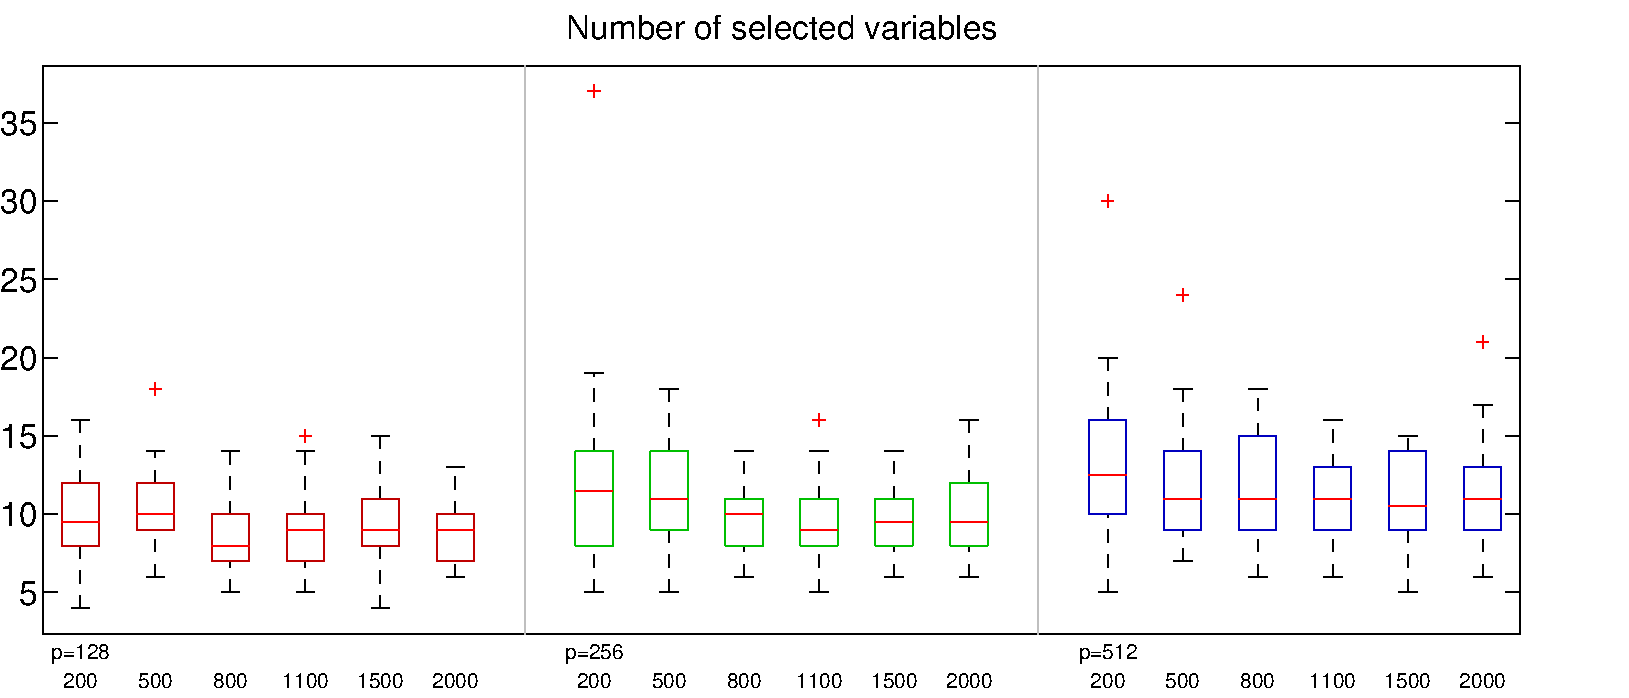
\includegraphics[width=0.42\textwidth]{figs/S_support_box} & \\
%(g) recovered support size for $p=256$ in (f) & (h) softmax $f_0$, correlated $X$, varying $s$ 
\end{tabular}
\end{center}
\caption{Support recovery results.}
\label{Support}
\vskip10pt
\end{figure*}

\begin{figure*}
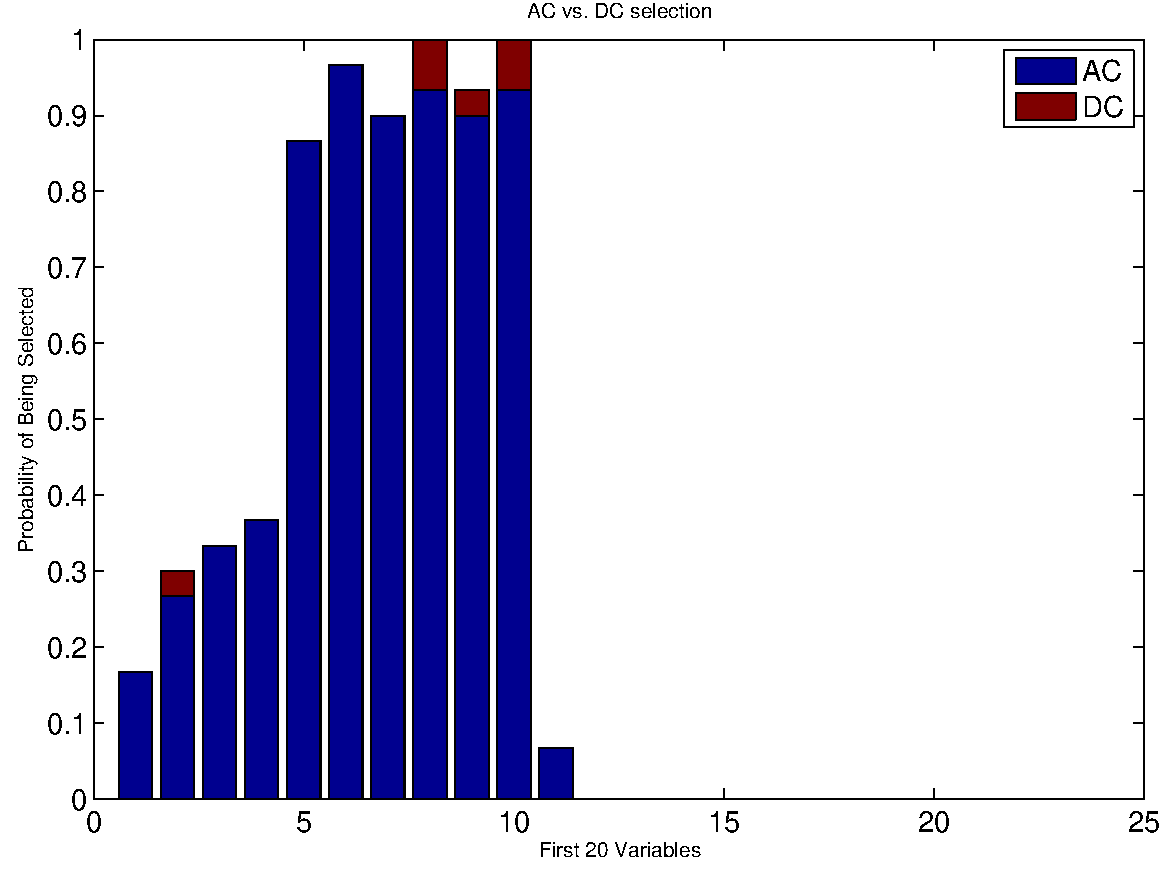
\includegraphics[width=0.5\textwidth]{figs/ACvDC}
\caption{Frequency of variable selection among the first 20 variables ($X_j$ for $j=1,...,20$) in the AC stage vs. in the DC stage. The true variables are [5,6,7,8,9,10].}
\label{fig:ac_v_dc}
\end{figure*}


\subsection{Boston housing data}

We next use the Boston housing data rather than simulated data. This data set
contains 13 covariates, 506 samples and one response variable
indicating housing values in suburbs of Boston. The data and detailed description
can be found on the UCI Machine Learning Repository website\footnote{\url{http://archive.ics.uci.edu/ml/datasets/Housing}}. 

We first use all $n=506$ samples (with standardization) in the AC/DC algorithm,
using a set of candidate regularization parameters $\{\lambda^{(t)}\}$
ranging from $\lambda^{(1)} = 0$ (no regularization) to $2$. For each $\lambda^{(t)}$
we obtain a function value matrix $\bds{f}^{(t)}$ with $p=13$
columns and $n=506$ rows. The non-zero columns in this matrix indicate the variables selected using $\lambda^{(t)}$.  

In Figure~\ref{Boston}(a), we plot on the y-axis the norm $\|\bds{f}^{(t)}_j\|_{\infty}$ of every column $j$ against the regularization strength $\lambda^{(t)}$. Instead of plotting the value of $\lambda^{(t)}$ on the x-axis however, we plot the total norm at $\lambda^{(t)}$ normalized against the total norm at $\lambda^{(1)}$: $\frac{\sum_j \|\bds{f}^{(t)}_j\|_{\infty}}{\sum_j \|\bds{f}^{(1)}\|_{\infty}}$. Thus, as x-axis moves from 0 to 1, the regularization goes from strong to weak. For comparison, we
plot the LASSO/LARS result in a similar way in Figure \ref{Boston}(b).
From the figures we observe that the first three variables selected by
AC/DC and LASSO are the same: \tts{LSTAT}, \tts{RM} and \tts{PTRATIO},
consistent with previous findings~\citep{SpAM:07}.  The fourth
variable selected by AC/DC is \tts{INDUS} (with $\lambda^{(t)}=0.7$).
We then refit AC/DC with only these four variables without
regularization, and plot the estimated additive functions in Figure
\ref{Boston}(d). When refitting, we constrain a component to be convex if it is non-zero in the AC stage and concave if it is non-zero in the DC stage. As can be seen, these functions contain clear
nonlinear effects which cannot be captured by LASSO. The shapes of
these functions, including the concave shape of the \tts{PTRATIO} function, are in agreement with those obtained by
SpAM~\citep{SpAM:07}. 

Next, in order to quantitatively study the predictive performance, we
run 3 times 5-fold cross validation, following the same procedure
described above---training, variable selection and refitting.  A plot
of the mean and standard deviation of the predictive mean squared
error (MSE) is shown in Figure \ref{Boston}(c). Since for AC/DC the same
regularization level $\lambda^{(t)}$ may lead to a slightly different number of selected
variables in different folds and runs, the values on the $x$-axis
for AC/DC are not necessarily integers. The figure clearly shows that AC/DC has a 
lower predictive MSE than LASSO.  We also compared the performance of
AC/DC with that of Additive Forward Regression (AFR) presented
in~\cite{Xi:09}, and found that they are similar.  The main advantages
of AC/DC compared with AFR and SpAM are that there are no smoothing
parameters required, and the optimization is formulated
as a convex program, guaranteeing a global optimum.

%\begin{figure}[!htpb]
%        \centering
%        \begin{subfigure}[b]{0.45\textwidth}
%                \centering
%                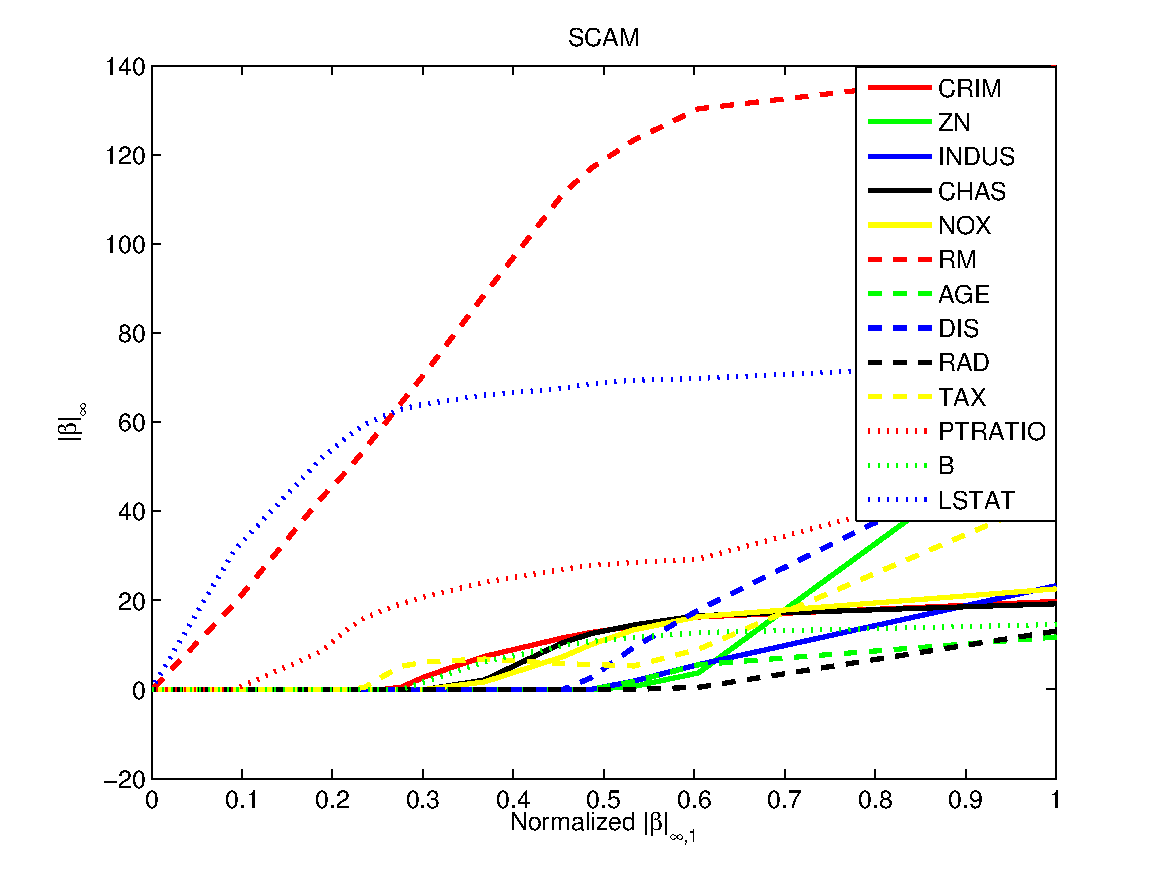
\includegraphics[width=\textwidth]{figs/Additive}
%                 \caption{Variable selection result using AC/DC.}
%                \label{AC/DC}
%        \end{subfigure}
%        \begin{subfigure}[b]{0.45\textwidth}
%                \centering
%                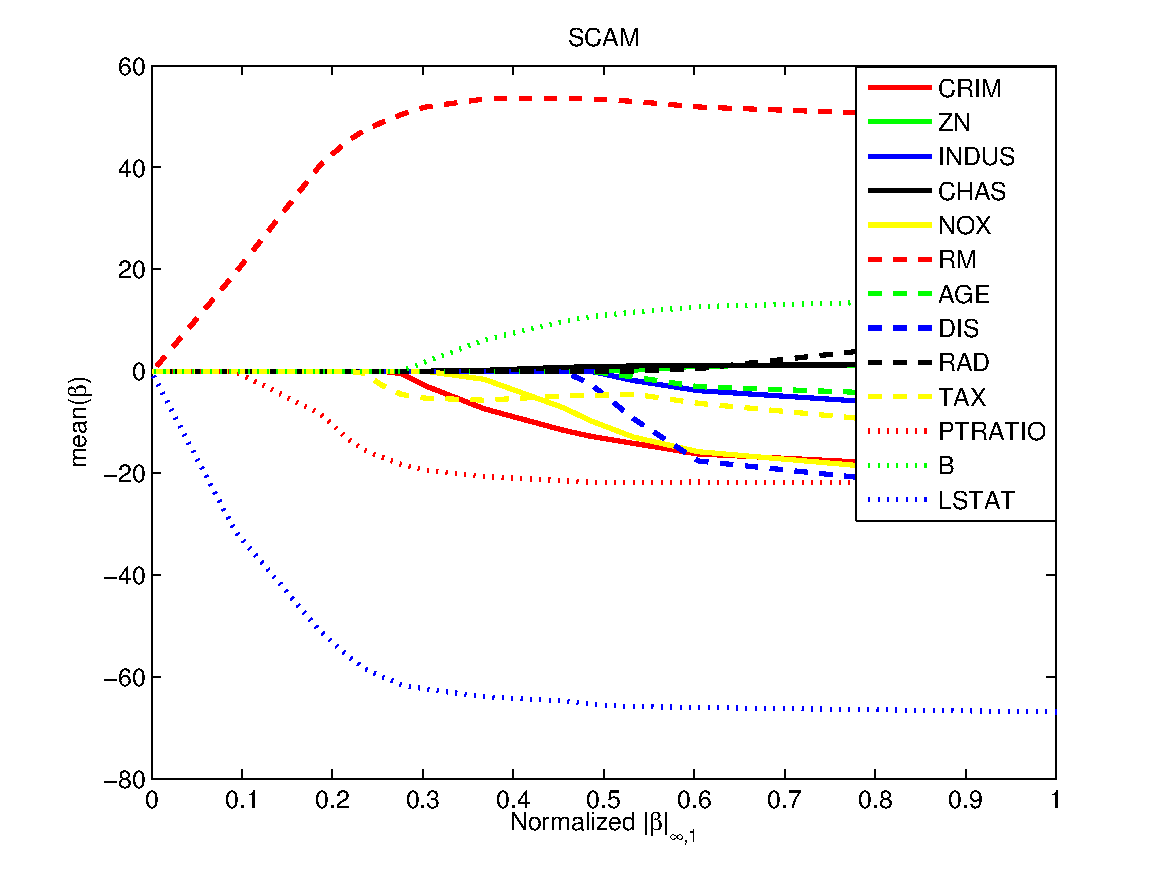
\includegraphics[width=\textwidth]{figs/Additive1}
%                 \caption{Variable selection result using AC/DC.}
%                \label{AC/DC1}
%        \end{subfigure}\\
%        \begin{subfigure}[b]{0.45\textwidth}
%                \centering
%                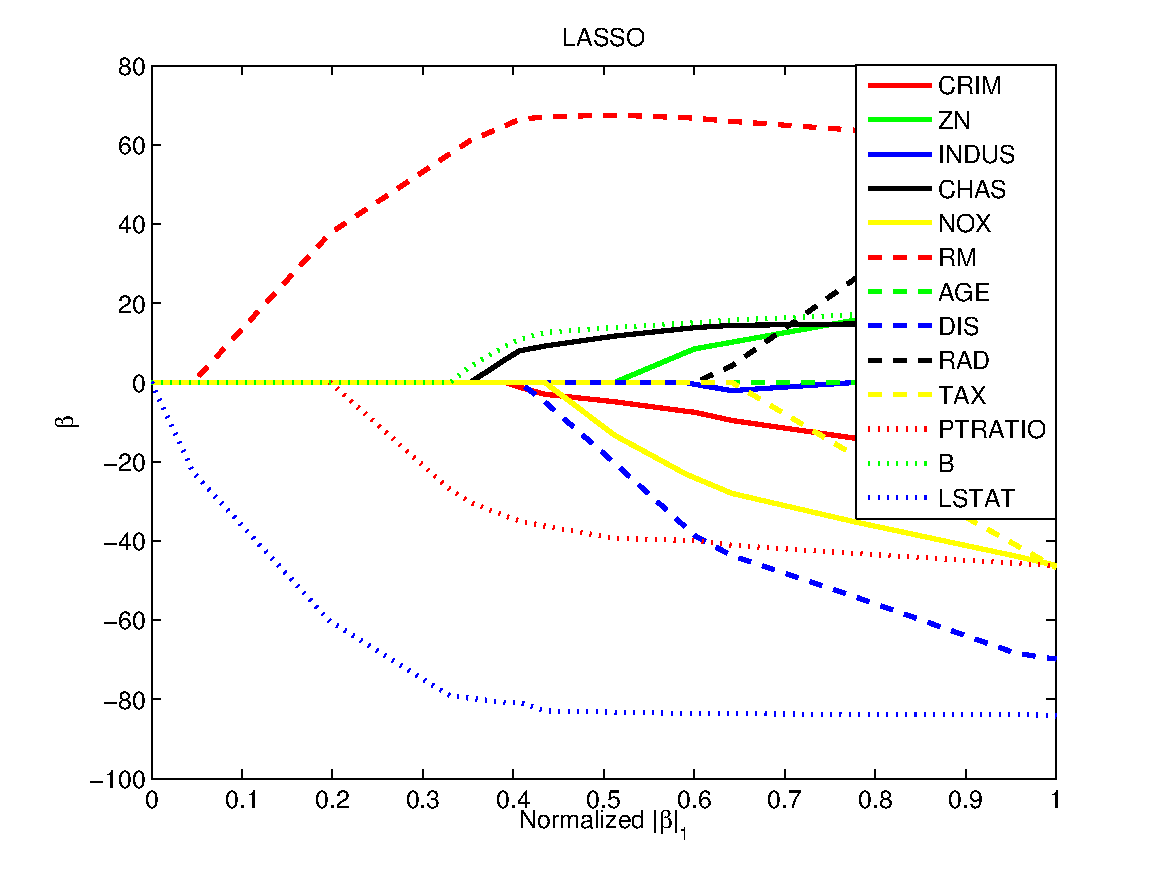
\includegraphics[width=\textwidth]{figs/LASSO}
%                \caption{Variable selection result using LASSO.}
%                \label{LASSO}
%        \end{subfigure}
%        \begin{subfigure}[b]{0.45\textwidth}
%                \centering
%                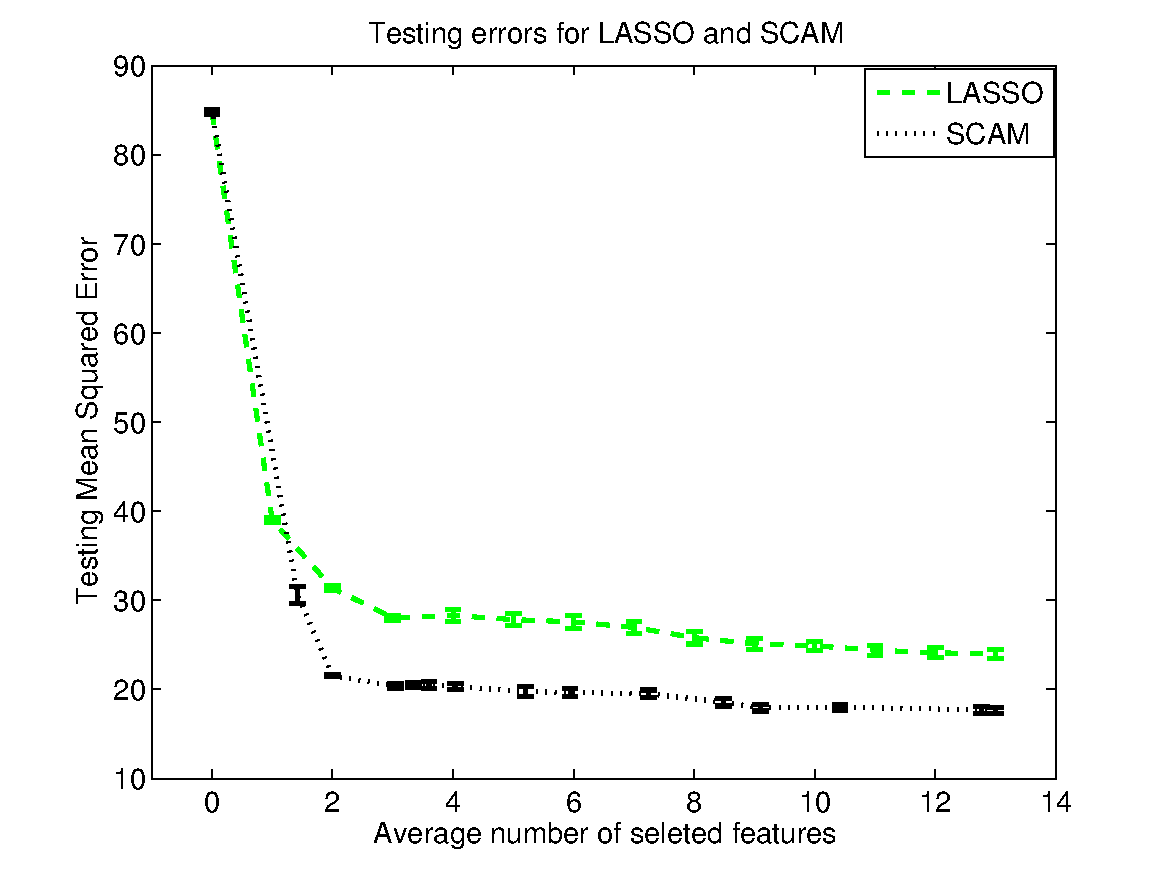
\includegraphics[width=\textwidth]{figs/MSE}
%                 \caption{Predictive MSE of AC/DC and LASSO.}
%                 \label{MSE}
%        \end{subfigure}\\
%        \begin{subfigure}[b]{0.45\textwidth}
%                \centering
%                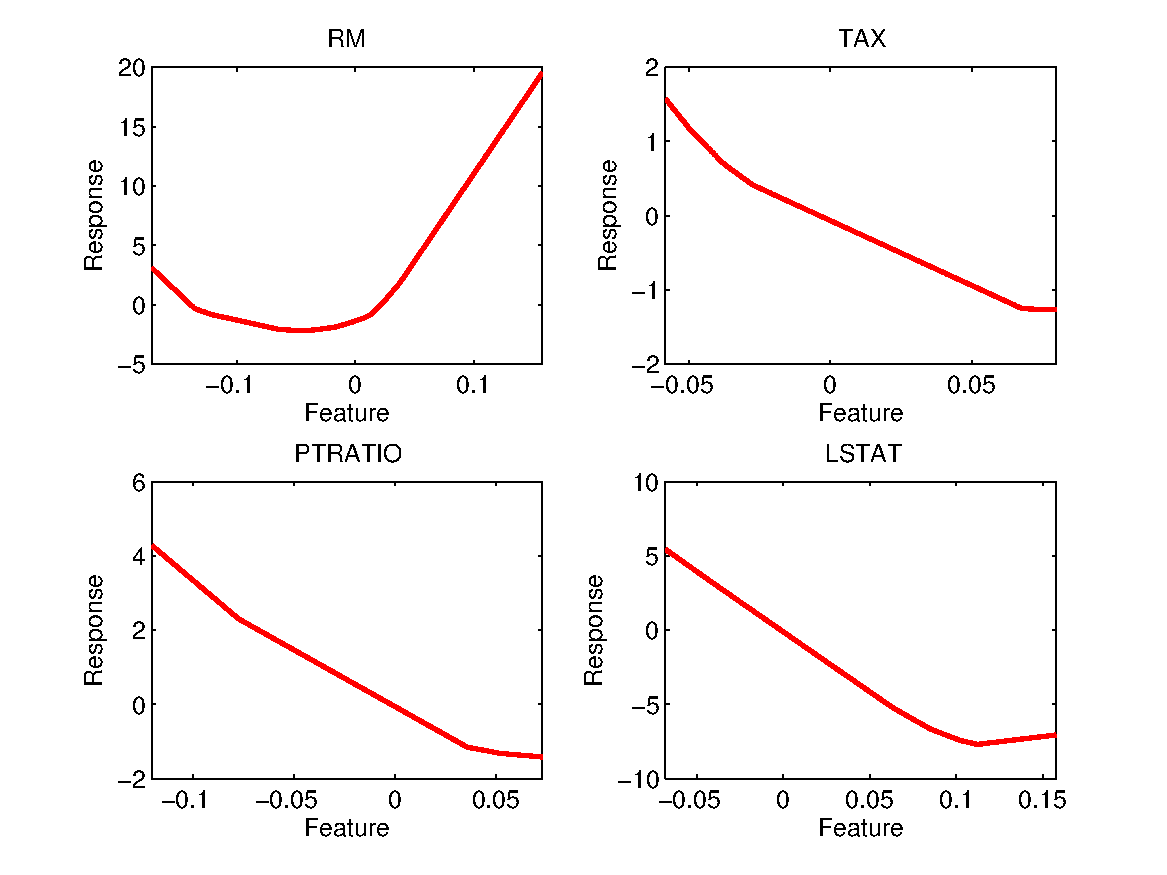
\includegraphics[width=\textwidth]{figs/Convex}
%                \caption{Inferred additive convex functions by AC/DC.}
%                \label{Convex}
%        \end{subfigure}
%        \caption{Results on Boston housing data.}\label{Boston}
%\end{figure}



\begin{figure*}
\begin{center}
\begin{tabular}{cc}
%\hskip-10pt
  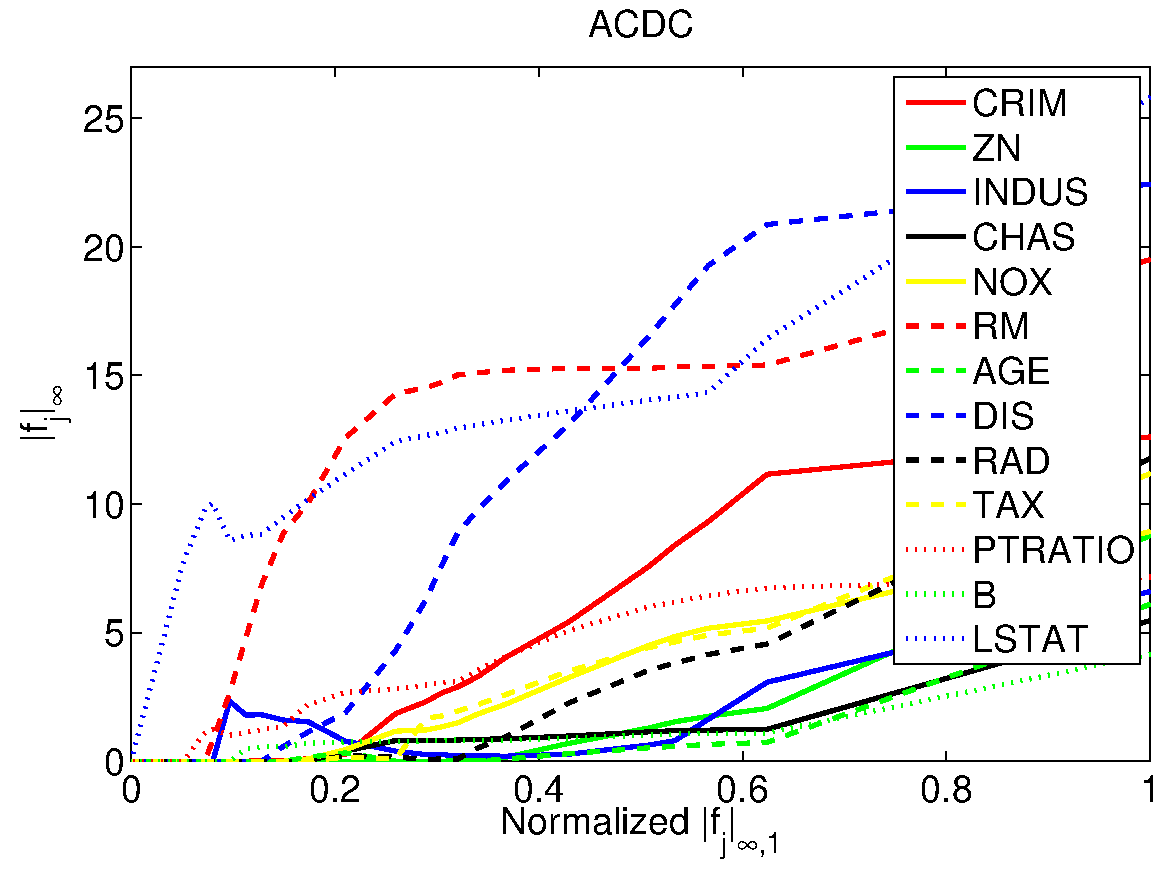
\includegraphics[width=.38\textwidth]{figs/acdc_path}  &
%\hskip-25pt
  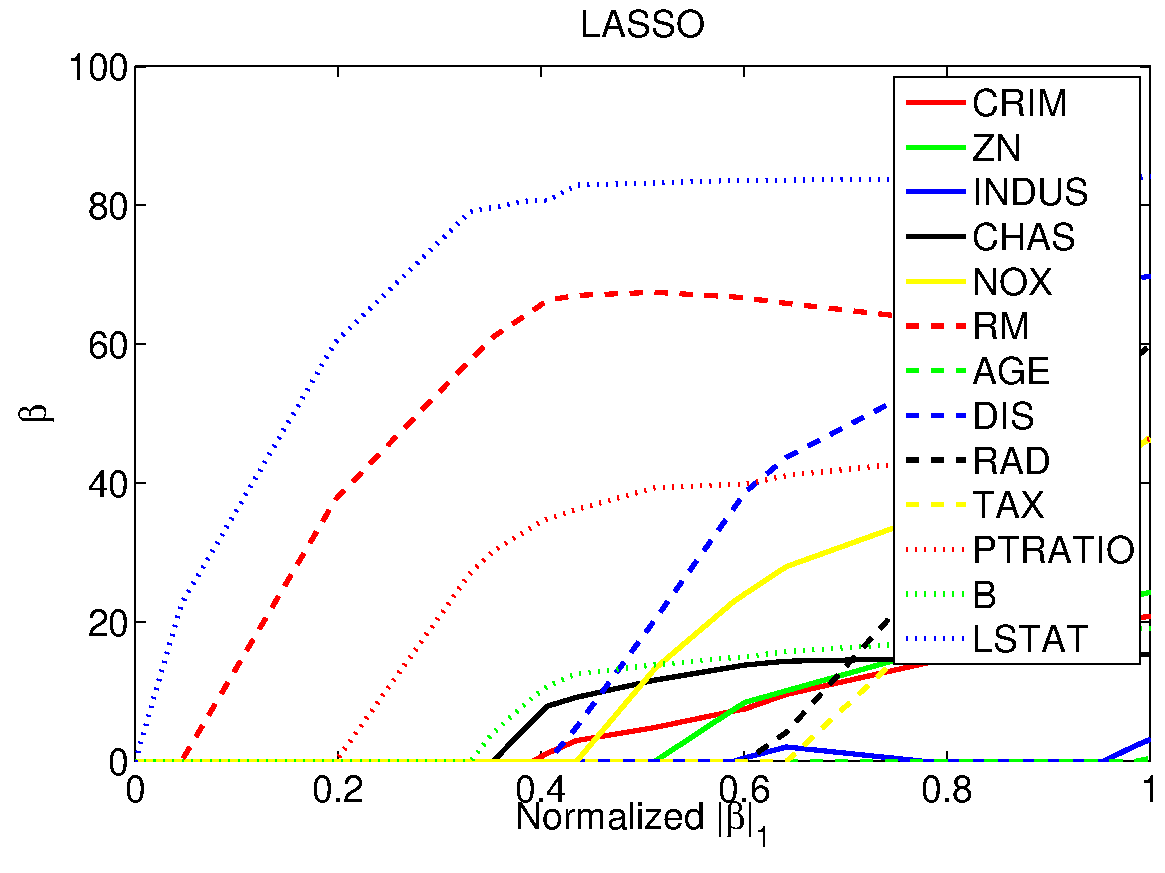
\includegraphics[width=.38\textwidth]{figs/lasso_path} 
\\
%\hskip-10pt 
(a) AC/DC $\|f_k\|_\infty$ paths & 
%\hskip-25pt
(b) LASSO $|\beta_k|$ paths \\
%\end{tabular}
%\begin{tabular}{cc}
  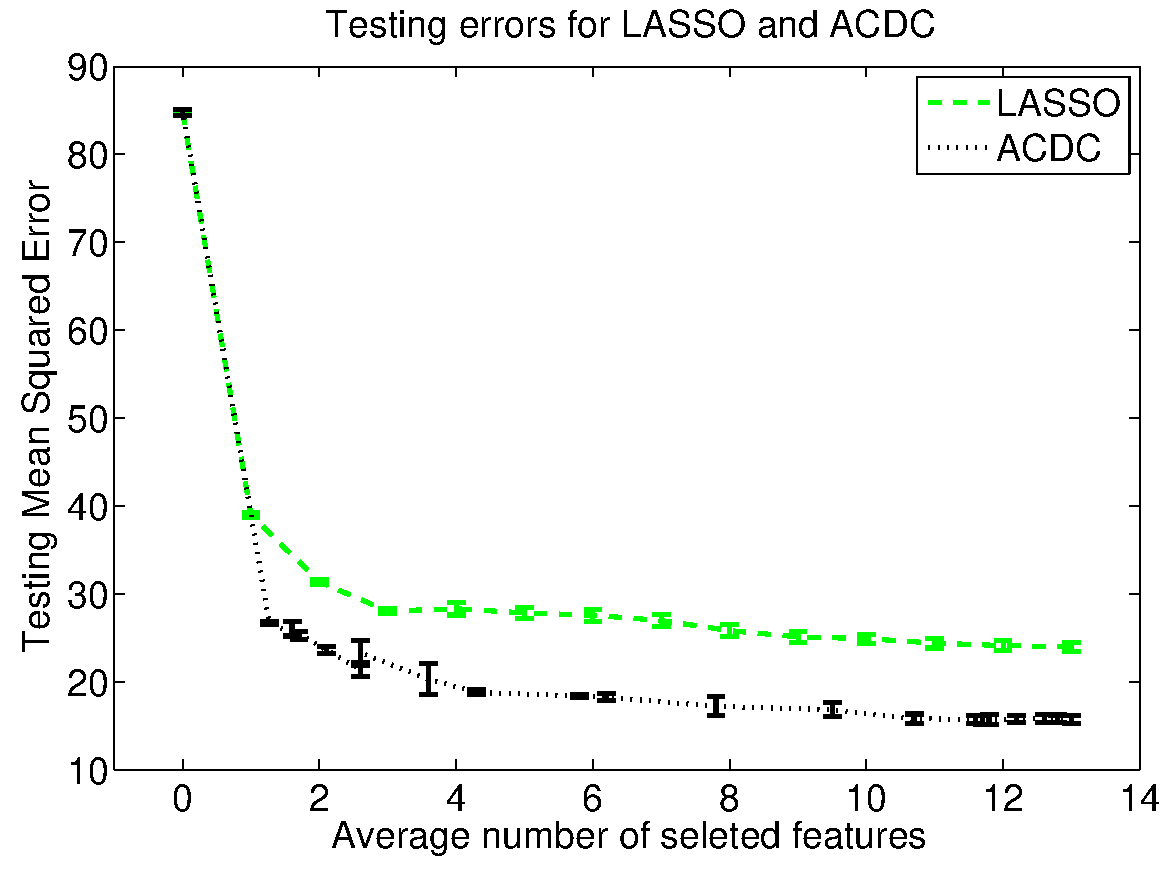
\includegraphics[width=.38\textwidth]{figs/MSEacdc} &
%\hskip 5pt
  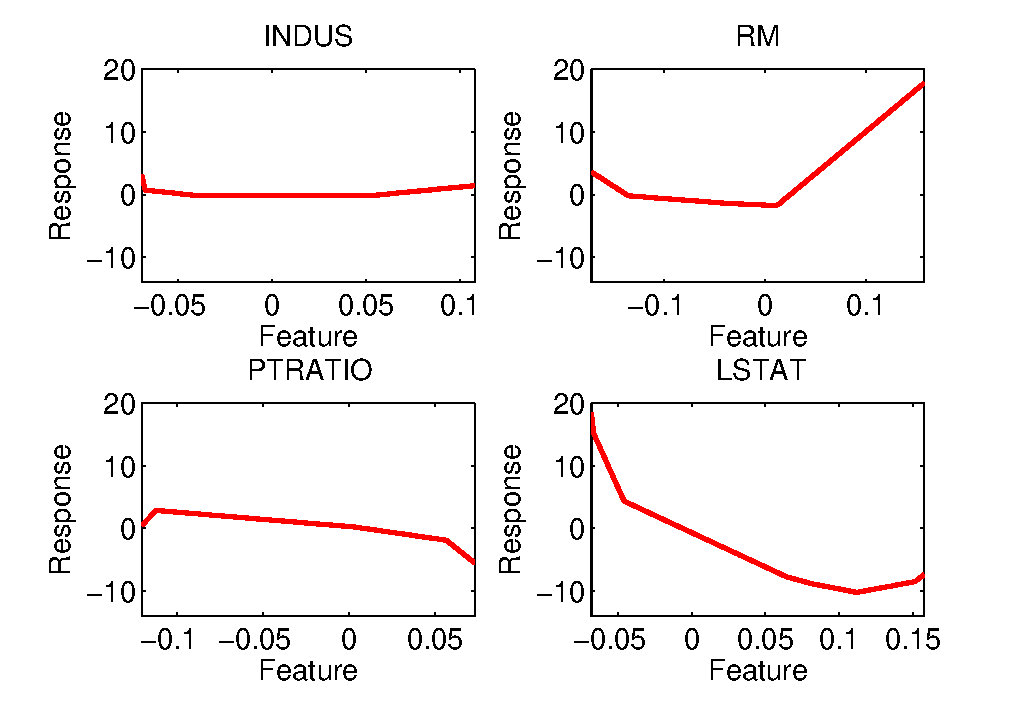
\includegraphics[width=.45\textwidth]{figs/acdc_functs}
\\
(c) predictive MSE & (d) estimated functions from AC/DC
\end{tabular}
\end{center}
\caption{Results on Boston housing data, showing regularization paths,
 MSE and fitted functions.} \label{Boston}
\end{figure*}


% DO NOT CHANGE; RefTex variables -minx
 
%%% Local Variables: ***
%%% mode:latex ***
%%% TeX-master: "paper-submit.tex" ***
%%% End: ***


\section{Discussion}

We have introduced a framework for estimating high dimensional but
sparse convex functions.  Because of the special properties of
convexity, variable selection for convex functions enjoys additive
faithfulness---it suffices to carry out variable selection over an
additive model, in spite of the approximation error this introduces.
Sparse convex additive models can be optimized using block coordinate
quadratic programming, which we have found to be effective and
scalable.  We established variable selection consistency results,
allowing exponential scaling in the ambient dimension.  We expect
that the technical assumptions we have used in these analyses can be
weakened; this is one direction for future work.  Another interesting
direction for building on this work is to allow for additive models that
are a combination of convex and concave components.  If the
convexity/concavity of each component function is known, this again
yields a convex program.  The challenge is to develop a method to
automatically detect the concavity or convexity pattern of the
variables.





\clearpage

%\bibliographystyle{plain}
\bibliography{local}

\newpage
\section{Appendix}
 
 
 \subsection{Proof of the Deterministic Condition for Sparsistency}
 \label{sec:deterministic_proof}
 
We restate Theorem~\ref{thm:deterministic} first for convenience. 
 
\begin{theorem} 
The following holds regardless of whether we impose the Lipschitz condition in optimization~\ref{opt:alternate_opt} and optimization~\ref{opt:alternate_opt_concave}.

Let $\{\hat{d}_k \}_{k \in S}$ be a minimizer of the restricted regression, that is, the solution to optimization (\ref{opt:alternate_opt}) where we restrict $k \in S$. 
Let $\hat{r} \coloneqq Y - \sum_{k \in S} \bar{\Delta}_k \hat{d}_k$ be the restricted regression residual. \\

Suppose for all $k\in S^c$, for all $i=1,...,n$, $\lambda_n > | \frac{1}{2n}
\hat{r}^\tran \mathbf{1}_{(i:n)}|$ where $\mathbf{1}_{(i:n)}$ is 1 on the coordinates of the $i$-th largest to the $n$-th largest entries of $X_k$ and 0 elsewhere.\\

Then the following are true:
\begin{enumerate}
\item Let $\hat{d}_k = 0$ for $k \in S^c$, then \{$\hat{d}_k\}_{k=1,...,p}$ is an optimal solution to optimization~\ref{opt:alternate_opt}. Furthermore, any solution to the optimization program \ref{opt:alternate_opt} must be zero on $S^c$.
\item For all $k \in S^c$, the solution to optimization~\ref{opt:alternate_opt_concave} must be 0 and must be unique.
\end{enumerate}
\end{theorem}


\begin{proof} 
We will omit the Lipschitz constraint in our proof here. It is easy to add that in and check that the result of the theorem still holds.\\

We first consider the first item in the conclusion of the theorem.

We will show that with $\{\hat{d}_k\}_{k=1,..,p}$ as constructed, we can set the dual variables to satisfy complementary slackness and stationary conditions: $\nabla_{d_k} \mathcal{L}(\hat{d})  = 0$ for all $k$.\\ 

The Lagrangian is
\begin{equation}
\label{eqn:full_lagrange}
\mathcal{L}( \{ d_k \}, \nu) = 
  \frac{1}{2n} \Big\| 
    Y - \sum_{k=1}^p  \bar{\Delta}_k d_k  \Big\|_2^2 + 
    \lambda \sum_{k=1}^p \| \bar{\Delta}_k d_k \|_\infty -
    \sum_{k=1}^p \sum_{i=2}^{n-1} \nu_{ki} d_{ki} 
\end{equation}
with the constraint that $\nu_{ki} \geq 0$ for all $k,i$.

Because $\{\hat{d}_k\}_{k \in S}$ is by definition the optimal solution of the restricted regression, it is a consequence that stationarity holds for $k \in S$, that is, $\partial_{ \{ d_k \}_{k \in S} } \mathcal{L}(d) = 0$, and that the dual variables $\nu_k$ for $k \in S$ satisfy complementary slackness.

We now verify that stationarity holds also for $k \in S^c$. We fix one dimension $k \in S^c$ and let $\hat{r} = Y - \sum_{k' \in S} \bar{\Delta}_{k'} \hat{d}_{k'}$. 

The Lagrangian form of the optimization, in term of just $d_k$, is
\[
\mathcal{L}(d_k, \nu_k) =
  \frac{1}{2n} \big\| Y - \sum_{k' \in S} \bar{\Delta}_{k'} d_{k'} 
  -  \bar{\Delta}_k d_k \big\|_2^2 
   + \lambda \| \bar{\Delta}_k d_k\|_\infty
  - \sum_{i=2}^{n-1} \nu_{ki} d_{ki}
\]
with the constraint that $v_i \geq 0$ for all $i$. 

The derivative of the Lagrangian is:
\begin{align*}
\partial_{d_k} \mathcal{L}(d_k) =  -\frac{1}{n} \bar{\Delta}_k^\tran ( Y - \sum_{k'\in S} \bar{\Delta}_{k'} d_{k'}  - \bar{\Delta}_k d_k )
        + \lambda \bar{\Delta}_k^\tran \mathbf{u}
      - \nu_k
\end{align*}
where $\mathbf{u}$ is the subgradient of $\| \bar{\Delta}_k d_k \|_\infty$, an $n$-vector such that $\| \mathbf{u}_T \|_1 = 1$ where $T = \{ i \,:\,  (\bar{\Delta}_k d_k)_i = \| \bar{\Delta}_k d_k \|_\infty \}$.

We now substitute in $d_{k'} = \hat{d}_{k'}$ for $k' \in S$, $d_k = 0$ for $k \in S$, and $r = \hat{r}$ and show that the duals can be set in a way to ensure that the derivatives are equal to 0.

\begin{align*}
\partial_{d_k} \mathcal{L}(\hat{d}_k) = -\frac{1}{n} \bar{\Delta}_k^\tran\hat{r} + \lambda \bar{\Delta}_k^\tran \mathbf{u}
           - \nu_k = 0 
\end{align*}
where $\| \mathbf{u} \| \leq 1$ and $\nu_k \geq 0$. It clear that to show stationarity, we only need to show that $-\frac{1}{n} \bar{\Delta}_k^\tran \hat{r} + \lambda \bar{\Delta}_k^\tran \mathbf{u} \geq 0$ hwere the inequality is element-wise.

Let us reorder the samples so that the $i$-th sample is the $i$-smallest sample. \\

We will construct $\gamma = 0$, and $\mathbf{u} = (-a, 0, ..., a)$ for some $0 < a < 1/2$. (coordinates of $\mathbf{u}$ correspond to the new sample ordering) We then just need to show that
\begin{align*}
- \frac{1}{n} \bar{\Delta}_k^\tran \hat{r} + \lambda \bar{\Delta}_k^\tran \mathbf{u} &\geq 0 \quad \Leftrightarrow \\
- \frac{1}{n} \Delta_k^\tran \hat{r} + \lambda \Delta_k^\tran \mathbf{u} &\geq 0 \quad \Leftrightarrow\\
- \frac{1}{n} \sum_{i > j} (X_{ki} - X_{kj}) \hat{r}_i + \lambda (X_{kn} - X_{kj})a &\geq 0 \quad 
   \textrm{for each } j \\
- \frac{1}{n} \sum_{i > j} \sum_{j < i' \leq i} \mathsf{gap}_{i'} \hat{r}_i 
    + \lambda (X_{kn} - X_{kj})a &\geq 0 \\
- \frac{1}{n} \sum_{i' > j} \mathsf{gap}_{i'} \sum_{i \geq i'} \hat{r}_i 
    + \lambda (X_{kn} - X_{kj})a &\geq 0 \\
- \frac{1}{n} \sum_{i' > j} \mathsf{gap}_{i'} \mathbf{1}_{(i':n)}^\tran \hat{r} 
   + \lambda (X_{kn} - X_{kj})a &\geq 0 
\end{align*}
where $\mathsf{gap}_i = X_{ki} - X_{k,i-1}$. If $\frac{1}{2n} |\mathbf{1}_{(i:n)}^\tran \hat{r}| \leq \lambda a$ for all $i=1,...,n$, then we have that:

\begin{align*}
- \frac{1}{n} \sum_{i' > j} \mathsf{gap}_{i'} \mathbf{1}_{i':n}^\tran \hat{r}
   + \lambda (X_{kn} - X_{kj})a &\geq 0 \quad \Leftrightarrow \\
- \sum_{i' > j} \mathsf{gap}_{i'} \lambda a + \lambda (X_{kn} - X_{kj}) a &\geq 0\\
- (X_{kn} - X_{kj}) \lambda a + \lambda (X_{kn} - X_{kj}) a &\geq 0
\end{align*}

We have thus proven that there exist one solution $\{ \hat{d}_k \}_{k=1,...,p}$ such that $\hat{d}_k = 0$ for all $k \in S^c$. Furthermore, we have shown that the subgradient variables $\mathbf{u}_k$ of the solution $\{ \hat{d}_k \}$ can be chosen such that $\| \mathbf{u}_k \|_1 < 1$ for all $k \in S^c$.  We now prove that if $\{ \hat{d}'_k \}_{k = 1,..., p}$ is another solution, then it must be that $\hat{d}'_k = 0$ for all $k \in S^c$ as well.  \\

%% prove uniqueness of sparsity pattern.

We first claim that $\sum_{k=1}^p \bar{\Delta}_k \hat{d}_k = \sum_{k=1}^p \bar{\Delta}_k \hat{d}'_k$. If this were not true, then a convex combination of $\hat{d}_k, \hat{d}'_k$ would achieve a strictly lower objective on the quadratic term. More precisely, let $\zeta \in [0,1]$. If $\sum_{k=1}^p \bar{\Delta}_k \hat{d}'_k \neq \sum_{k=1}^p \bar{\Delta}_k \hat{d}_k$, then $\| Y - \sum_{k=1}^p \bar{\Delta}_k \big( \hat{d}_k + \zeta ( \hat{d}'_k - \hat{d}_k) \big) \|_2^2$ is strongly convex as a function of $\nu$. Thus, it cannot be that $\hat{d}_k$ and $\hat{d}'_k$ both achieve optimal objective and we have reached a contradiction.\\

Now, we look at the stationarity condition for both $\{ \hat{d}_k \}$ and $\{ \hat{d}'_k \}$. Let $\mathbf{u}_k \in \partial \| \bar{\Delta}_k \hat{d}_k \|_\infty$ and let $\mathbf{u}'_k \in \partial \| \bar{\Delta}_k \hat{d}'_k \|_\infty$ be the two sets of subgradients. Let $\{ \nu_{ki} \}_{k=1,..,p,\, i=1,...n-1}$ and $\{ \nu'_{ki} \}$ be the two sets of positivity dual variables. \footnote{since there is no positivity constraint on $d_{k1}$, we let $\nu_{k1} = 0$ always.}

Let us define $\bar{\Delta}$, a $n \times p(n-1)$ matrix, to denote the column-wise concatenation of $\{ \bar{\Delta}_k \}_k$ and $\hat{d}$, a $p(n-1)$ dimensional vector, to denote the concatenation of $\{ \hat{d}_k \}_k$. With this notation, we can express $\sum_{k=1}^p \bar{\Delta}_k \hat{d}_k = \bar{\Delta} \hat{d}$.

Since both solutions $(\hat{d}, \mathbf{u}, \nu)$ and $(\hat{d}', \mathbf{u}', \nu')$ must satisfy the stationarity condition, we have that:
\[
\bar{\Delta}^\tran ( Y - \bar{\Delta} \hat{d} ) 
   + \lambda \sum_{k=1}^p \bar{\Delta}_k^\tran \mathbf{u}_k - \nu = 
\bar{\Delta}^\tran ( Y - \bar{\Delta} \hat{d}' ) 
   + \lambda \sum_{k=1}^p \bar{\Delta}_k^\tran \mathbf{u}'_k - \nu' = 0
\] 
We multiply both sides of the above equation by $\hat{d}'$:
\[
\hat{d}'^{\tran}  \bar{\Delta}^\tran ( Y - \bar{\Delta} \hat{d} ) 
    + \lambda \sum_{k=1}^p \hat{d}'^\tran_k \bar{\Delta}_k^\tran \mathbf{u}_k - \hat{d}'^\tran \nu = \hat{d}'^{\tran}  \bar{\Delta}^\tran ( Y - \bar{\Delta} \hat{d}' ) 
    + \lambda \sum_{k=1}^p \hat{d}'^\tran_k \bar{\Delta}_k^\tran \mathbf{u}'_k - \hat{d}'^\tran \nu'
\]
Since $\bar{\Delta} \hat{d}_k = \bar{\Delta} \hat{d}$, $\hat{d}'^\tran \nu' = 0$ (complementary slackness), and $\hat{d}'^\tran_k \bar{\Delta}_k^\tran \mathbf{u}'_k  = \| \hat{f}'_k \|_\infty$ (where $\hat{f}'_k = \bar{\Delta}_k \hat{d}'_k$), we have that:
\[
\lambda \sum_{k=1}^p \hat{d}'^\tran_k \bar{\Delta}_k^\tran \mathbf{u}_k - \hat{d}'^\tran \nu = \lambda \sum_{k=1}^p \| \hat{f}'_k \|_\infty
\]
On one hand, $\hat{d}'$ is a feasible solution so $\hat{d}'^\tran \nu \geq 0$ and so 
\[
\sum_{k=1}^p \hat{d}'^\tran_k \bar{\Delta}_k^\tran \mathbf{u}_k \geq \sum_{k=1}^p \| \hat{f}'_k \|_\infty .
\]

On the other hand, by Holder's inequality:
\begin{align*}
\sum_{k=1}^p \hat{d}'^\tran_k \bar{\Delta}_k^\tran \mathbf{u}_k &\leq 
   \sum_{k=1}^p \| \hat{f}'_k \|_\infty \|\mathbf{u}_k \|_1 
\end{align*}

Since $\mathbf{u}_k$ can be chosen so that $\| \mathbf{u}_k \|_1 < 1$ for all $k \in S^c$, we would get a contradiction if $\| \hat{f}'_k \|_\infty > 0$ for some $k \in S^c$. We thus conclude that $\hat{d}'$ must follow the same sparsity pattern.\\


The second item in the theorem concerning optimization~\ref{opt:alternate_opt_concave} is proven in exactly the same way. 

The Lagrangian of optimization~\ref{opt:alternate_opt_concave} is:
\[
\mathcal{L}_{\trm{cave}}(d_k, \nu_k) = 
  \frac{1}{2n} \big\| \hat{r} - \bar{\Delta}_k d_k \big \|_2^2 + 
  \lambda \| \bar{\Delta}_k d_k \|_\infty + \sum_{k=1}^p \sum_{i=2}^{n-1} \nu_{ki} d_{ki}
\]

The exact same reasoning applies to show that $\hat{d}_k = 0$ satisfies KKT conditions sufficient for optimality.

\end{proof}
 
 
 
 
 
 
 \subsection{Proof of False Positive Control}
 \label{sec:false_positive_proof}
 
\textbf{Note:} the symbols $c,C$ represent absolute constants. We will often abuse notation and ``absorb'' new absolute constants into $c, C$; the actual value of $c, C$ could thus vary from line to line.

 We first restate the theorem for convenience. 
 

\begin{theorem} 
Suppose assumptions A1-A4 hold. Suppose $\sqrt{\log 2np} \geq 1$. Define $\tilde{\sigma} \equiv \max(\sigma, B)$.

Suppose $\lambda_n \geq 8 s \tilde{\sigma}  \sqrt{ \frac{1}{n} \log^2 np}$, then, with probability at least $ 1 - \frac{12}{n}$, for all $k \in S^c$, and for all $i'=1,...,n$:
\[
\lambda_n > \Big| \frac{1}{2n}\hat{r}^\tran \mathbf{1}_{(i':n)_k} \Big|
\]

And therefore,for all $k \in S^c$, both the AC solution $\hat{f}_k$, from optimization~\ref{opt:alternate_opt}, and the DC solution $\hat{g}_k$, from optimization~\ref{opt:alternate_opt_concave} are zero. 
\end{theorem}

\begin{proof}
The key is to note that $\hat{r}$ and $\Delta_{k,j}$ are independent for all $k \in S^c,j=1,...,n$ because $\hat{r}$ is only dependent on $X_{S}$.

Fix $j$ and $i$. $\hat{r}^\tran \mathbf{1}_{(i':n)_k}$ is then the sum of $n-i'+1$ random coordinates of $\hat{r}$. We will then use Serfling's theorem on the concentration of measure of sampling without replacement. (corollary~\ref{cor:serfling}) We must first bound $\| \hat{r} \|_\infty$ and $\frac{1}{n} \sum_{i=1}^n \hat{r}_i$ before we can use Serfling's results however.\\

\textbf{Step 1}: Bounding $\| \hat{r} \|_\infty$. 

$\hat{r}_i = f_0(x_i) + w_i - \hat{f}(x_i)$ where $\hat{f}(x_i) = \sum_{k \in S} \bar{\Delta}_k \hat{d}_k$ is the convex additive function outputted by the restricted regression.

Both $f_0(x_i)$ and $\hat{f}(x_i)$ are bounded by $sB$.

Because $w_i$ is subgaussian, $|w_i| \leq  \sigma \sqrt{2\log \frac{2}{\delta}}$ with probability at most $1-\delta$. By union bound across $i=1,...,n$, we have that $\| w\|_\infty \leq \sigma \sqrt{ 2 \log \frac{2n}{\delta}}$ with probability at most $1 - \delta$.

We now put this together: 
%and take another union bound across all $j$ and all $i'$:
\begin{align}
\| \hat{r} \|_\infty &\leq 2sB + \sigma \sqrt{ 2\log \frac{2n}{\delta}}) \nonumber \\
      &\leq 4 s \tilde{\sigma} \sqrt{\log \frac{2n}{\delta}} \label{eqn:stepone_rhat}
\end{align}
with probability at least $1 - \delta$. We define $\tilde{\sigma} = \max(\sigma, B)$. We also supposed that $\sqrt{\log \frac{2np}{\delta}} \geq 1$, which is acceptable since $\delta \leq 1$ and the theorem presupposes that $\sqrt{ \log 2np } \geq 1$.

\textbf{Step 2}: Bounding $| \frac{1}{n} \hat{r}^\tran \mathbf{1} |$. 

\begin{align*}
\frac{1}{n} \hat{r}^\tran \mathbf{1} &= 
    \frac{1}{n} \sum_{i=1}^n f_0(x_i) + w_i - \hat{f}(x_i) \\
  &= \frac{1}{n} \sum_{i=1}^n f_0(x_i) + w_i \quad \trm{ ($\hat{f}$ is centered)}
\end{align*}

Because $|f_0(x_i)| \leq sB$, the first term $| \frac{1}{n} \sum_{i=1}^n f_0(x_i)|$ is at most $sB \sqrt{\frac{2}{n} \log \frac{2}{\delta}}$ with probability at most $1-\delta$ by Hoeffding Inequality.

Because $w_i$ is subgaussian, the second term $|\frac{1}{n} \sum_{i=1}^n w_i|$ is at most $\sigma \sqrt{ \frac{2}{n} \log \frac{2}{\delta}}$ with probability at most $1-\delta$.

Taking an union bound, we have that 

\begin{align}
| \frac{1}{n} \hat{r}^\tran \mathbf{1}| &\leq sB \sqrt{\frac{2}{n} \log \frac{4}{\delta}} +  \sigma \sqrt{\frac{2}{n} \log \frac{4}{\delta}} \nonumber \\
  &\leq 4 s \tilde{\sigma} \sqrt{\frac{1}{n} \log \frac{4}{\delta}} \label{eqn:steptwo_rhat}
\end{align}
with probability at least $1-\delta$.\\

\textbf{Step 3}: We now apply Serfling's theorem.

For any $k \in S^c$, Serfling's theorem states that with probability at least $1 - \delta$:
\begin{align*}
\Big
|\frac{1}{n} \hat{r}^\tran \mathbf{1}_{(i':n)_k}\Big| \leq
   2\| \hat{r} \|_\infty \sqrt{ \frac{1}{n} \log \frac{2}{\delta}} + 
   \Big|\frac{1}{n} \hat{r}^\tran \mathbf{1} \Big|
\end{align*}

We need Serfling's theorem to hold for all $k = 1,...,p$ and $i' = 1,...,n$. We also need the events that $\|\hat{r}\|_\infty$ and $| \frac{1}{n} \hat{r}^\tran \mathbf{1}|$ are small to hold. The following follows from a union bound. With probability at least $1-\delta$, for all $k,i'$,
\begin{align*}
\Big
|\frac{1}{n} \hat{r}^\tran \mathbf{1}_{(i':n)_k}\Big| &\leq
   2\| \hat{r} \|_\infty \sqrt{ \frac{1}{n} \log \frac{6np}{\delta}} + 
   \Big|\frac{1}{n} \hat{r}^\tran \mathbf{1} \Big|\\
  &\leq 4s\tilde{\sigma}\sqrt{\log \frac{6n}{\delta}} \sqrt{\frac{1}{n}\log \frac{6np}{\delta}} + 4 s \tilde{\sigma} \sqrt{\frac{1}{n}\log \frac{12}{\delta}} \\
  &\leq 8 s\tilde{\sigma} \sqrt{ \frac{1}{n} \log^2 \frac{12np}{\delta}}
\end{align*}

In the second inequality, we used equation~\ref{eqn:stepone_rhat} and equation~\ref{eqn:steptwo_rhat} from step 1 and 2 respectively. Setting $\delta = \frac{12}{n}$ gives the desired result.


\end{proof}

 
 
%%%%%%%%%%%%%%%%%%%%%%%%%%%%%%
%%
%%
%%
%%
%%%%%%%%%%%%%%%%%%%%%%%%%%%%%% 
 
 \subsection{Proof of False Negative Control}
 \label{sec:false_negative_proof}
 
\textbf{Note:} the symbols $c,C$ represent absolute constants. We will often abuse notation and ``absorb'' new absolute constants into $c, C$; the actual value of $c, C$ could thus vary from line to line.

 We first introduce notations.
 \subsubsection{Notation} 
\label{sec:false_negative_proof_notations}

Let $f : \mathbb{R}^s \rightarrow \R$, we denote $\| f \|_P \equiv \E f(X)^2$. \\
Given samples $X_1,...,X_n$, we denote $\| f \|_n \equiv \frac{1}{n} \sum_{i=1}^n f(X_i)^2$ and $\langle f, g \rangle_n \equiv \frac{1}{n} \sum_{i=1}^n f(X_i) g(X_i)$. \\

Let $\mathcal{C}^1$ denote the set of univariate convex functions supported on $[-b,b]$. Let $\mathcal{C}^1_B \equiv \{ f \in \mathcal{C}^1 \,:\, \| f \|_\infty \leq B \}$ denote the set of $B$-bounded univariate convex functions. \\

Define $\mathcal{C}^s$ as the set of convex additive functions and $\mathcal{C}^s_B$ likewise as the set of convex additive functions whose components are $B$-bounded.
\begin{align*}
\mathcal{C}^s &\equiv \{ f \,:\, f = \sum_{k=1}^s f_k, \,
   f_k \in \mathcal{C}^1 \} \\
\mathcal{C}^s_B &\equiv \{ f \in \mathcal{C}^s \,:\, 
f = \sum_{k=1}^s f_k, \, \| f_k \|_\infty \leq B \}
\end{align*}

Let $f^*(x) = \sum_{k=1}^s f^*_k(x_k)$ be the population risk minimizer:
\[
f^* = \arg\min_{f \in \mathcal{C}^s} \| f_0 - f^* \|_P^2
\]

We let $sB$ be an upper bound on $\| f_0 \|_\infty$ and $B$ be an upper bound on $\| f^*_k \|_\infty$. It follows that $\|f^* \|_\infty \leq s B$.

We define $\hat{f}$ as the empirical risk minimizer:
\[
\hat{f} = \arg\min \Big \{ \| y - f \|_n^2 + \lambda \sum_{k=1}^s \| f_k \|_\infty 
    \,:\, f \in \mathcal{C}^s_B,\, \mathbf{1}_n^\tran f_k = 0 \Big \}
\]

For $k \in \{1,...,s\}$, define $g^*_k$ to be decoupled concave population risk minimizer
\[
g^*_k \equiv \argmin_{g_k \in \mh \mathcal{C}^1} \| f_0 - f^* - g_k \|_P^2 
\]
In our proof, we will analyze $g^*_k$ for $k$'s such that $f^*_k = 0$. Likewise, we define the empirical version:
\[
\hat{g}_k \equiv \argmin \Big\{ \| f_0 - \hat{f} - g_k \|_n^2 \,:\, g_k \in \mh \mathcal{C}^1_B \,, \mathbf{1}_n^\tran g_k = 0 \Big\}
\]
By the definition of the ACDC procedure, $\hat{g}_k$ exist only for $k$ that have zero in their convex additive approximation.


\subsubsection{Proof}
 
By additive faithfulness of the ACDC procedure, it is necessary that $f^*_k \neq 0$ or $g^*_k \neq 0$ for all $k \in S$. \\


Intuitively, we would like to show the following:
\begin{align*}
\| f_0 - \hat{f} \|_P & \approx \| f_0 - f^* \|_P \\
\| f_0 - f^* - \hat{g}_k \|_P & \approx \| f_0 - f^* - g^*_k \|_P 
       \quad \trm{for all $k \in S$ where $f^*_k = 0$}
\end{align*}
where the estimation error is a term that decreases with $n$.

Suppose $\hat{f}_k = 0$ and $f^*_k \neq 0$, then, when $n$ is large enough, there must exist a contradiction because the population risk of $f^*$, $\| f_0 - f^* \|_P$, is strictly larger than the population risk of the best approximation whose $k$-th component is constrained to be zero. 

Suppose $f^*_k = 0$, then $g^*_k \neq 0$. When $n$ is large enough, $\hat{g}_k$ must not be zero or we would have another contradiction. \\


\begin{theorem}
\label{thm:convex_consistent}
Let $\tilde{\sigma} \equiv \max(\sigma, B)$. Let $\hat{f}$ be the minimizer of the restricted regression with $\lambda \leq 9 s \tilde{\sigma} \sqrt{ \frac{1}{n} \log^2 np}$.

Suppose $n \geq c_1 \max(\sqrt{sB}, B)$.

Then, with probability at least $1-\frac{C}{n}$,
\begin{align}
\|f_0 - \hat{f} \|_P^2 - \| f_0 - f^* \|_P^2 
&\leq c B^2 \tilde{\sigma} \sqrt{ \frac{s^5}{n^{4/5}} \log^2 np}
\end{align}
Where $c, C$ are constants, possibly dependent on $c_1, b$.

\end{theorem}


\begin{proof}

\textbf{Step 1.} We start from the definition. 

\begin{align*}
\| y - \hat{f} \|_n^2 + \lambda \sum_{k=1}^s \| \hat{f}_k \|_\infty &\leq
  \| y - f^* + \bar{f}^* \|_n^2 + \lambda \sum_{k=1}^s \| f^*_k - \bar{f}^* \|_\infty 
\end{align*}
We plug in $y = f_0 + w$:
\begin{align*}
\| f_0 + w - \hat{f} \|_n^2 + \lambda \sum_{k=1}^s \Big( \| \hat{f}_k \|_\infty - 
    \| f^*_k - \bar{f}^*_k \|_\infty \Big) &\leq \|f_0 + w - f^* + \bar{f}^* \|_n^2 \\
\| f_0 - \hat{f} \|_n^2 + 2\langle w, f_0 - \hat{f} \rangle_n 
     +\lambda \sum_{k=1}^s \Big( \| \hat{f}_k \|_\infty - \|f^*_k -\bar{f}^*_k\|_\infty \Big) 
    &\leq \| f_0 - f^* + \bar{f}^* \|_n^2 + 
    2 \langle w, f_0 - f^* + \bar{f}^* \rangle \\
\|f_0 - \hat{f} \|_n^2 - \| f_0 - f^* + \bar{f}^* \|_n^2 + 
    \lambda \sum_{k=1}^s \Big( \| \hat{f}_k \|_\infty - 
 \| f^*_k - \bar{f}^*_k \|_\infty \Big) &\leq 2 \langle w, \hat{f} - f^* + \bar{f}^* \rangle
\end{align*}

The middle term can be bounded with the assumption that $\|f^*_k - \bar{f}^*_k \|_\infty \leq 2B$.

\begin{align*}
\|f_0 - \hat{f} \|_n^2 - \| f_0 - f^* + \bar{f}^* \|_n^2 
   &\leq 2 \langle w, \hat{f} - f^* + \bar{f}^* \rangle + \lambda 2 s B 
\end{align*}

Using Lemma~\ref{lem:remove_centering}, we can remove $\bar{f}^*$ from the LHS. With probability at least $1 - \delta$:
\begin{align}
\label{eqn:first_step_inequality}
\|f_0 - \hat{f} \|_n^2 - \| f_0 - f^* \|_n^2 
   &\leq 2 \langle w, \hat{f} - f^* + \bar{f}^* \rangle + \lambda 2 s B + c(sB)^2 \frac{1}{n} \log \frac{2}{\delta}
\end{align}

%[TOOD: at this point, we still have to choose a value for $\lambda$]\\

%%%%%%%%%%%%%%%%%%%%%%%%%%%%%%
%% 
%% Step 2
%%
%%
%%%%%%%%%%%%%%%%%%%%%%%%%%%%%%

\textbf{Step 2.} We upper bound $2 \langle w, \hat{f} - f^* + \bar{f}^* \rangle$ with bracketing entropy.

Define $\mathcal{G}$ as $\{ f - f^* + \bar{f}^* \,:\, f \in \mathcal{C}^s_B \}$ as the set of convex additive functions centered around the function $f^* - \bar{f}^*$. 

By Corollary~\ref{prop:convexbracket_lp}, there is an $\epsilon$-bracketing of $\mathcal{G}$ whose size is bounded by $\log N_{[]}( 2\epsilon, \mathcal{G}, L_1(P)) \leq sK^{**} \left( \frac{2sbB}{\epsilon} \right)^{1/2}$, for all $\epsilon \in (0, sB \epsilon_3]$.

Let us suppose condition~\ref{cond:simplify_covering_number} holds, then, by Corollary~\ref{cor:convexbracket_ln}, with probability at least $1-\delta$, each bracketing pair $(h_U, h_L)$ is close in $L_1(P_n)$ norm, i.e., for all $(h_U, h_L)$, 
$\frac{1}{n} \sum_{i=1}^n | h_U(X_i) - h_L(X_i) | \leq 2 \epsilon + sB \sqrt{ \frac{sK^{**}(2sbB
)^{1/2} \log \frac{1}{\delta}}{2\epsilon^{1/2} n}}$. We verify at the end of the proof that condition~\ref{cond:simplify_covering_number} indeed holds.


For each $h \in \mathcal{G}$, there exists a pair $(h_U, h_L)$ such that $h_U(X_i) - h_L(X_i) \geq h(X_i) - h_L(X_i) \geq 0$. Therefore, with probability at least $1-\delta$, uniformly for all $h \in \mathcal{G}$:

$$
\frac{1}{n} \sum_{i=1}^n |h(X_i) - h_L(X_i)| \leq \frac{1}{n} \sum_{i=1}^n | h_U(X_i) - h_L(X_i)| \leq 2\epsilon +  (sB) \sqrt{ \frac{sK^{**}(2sbB)^{1/2} \log \frac{1}{\delta}}{2\epsilon^{1/2} n}}
$$.

We denote $\epsilon_{n,\delta} \equiv (sB) \sqrt{ \frac{sK^{**}(2sbB)^{1/2} \log \frac{1}{\delta}}{2\epsilon^{1/2} n}}$. Let $\mathcal{E}_{[\,]}$ denote the event that for each $h \in \mathcal{G}$, there exists $h_L$ in the $\epsilon$-bracketing such that $\|h-h_L\|_{L_{P_n}} \leq 2\epsilon + \epsilon_{n, \delta}$. $\mathcal{E}_{[\,]}$ has probability at most $1-\delta$ as shown.\\

Let $\mathcal{E}_{\|w\|_\infty}$ denote the event that $\| w \|_\infty \leq \sigma \sqrt{ 2\log \frac{2n}{\delta}}$; $\mathcal{E}_{\|w\|_\infty}$ has probability at most $1-\delta$. We take an union bound between $\mathcal{E}_{\|w\|_\infty}$ and $\mathcal{E}_{[\,]}$ and get that, with probability at most $1-2\delta$, for all $h$:
\[
|\langle w, h - h_L\rangle_n| \leq \| w \|_\infty \frac{1}{n} \sum_{i=1}^n |h(X_i) - h_L(X_i)| \leq
  \sigma \sqrt{2 \log \frac{4n}{\delta}} \left( \epsilon + \epsilon_{n,2\delta} \right)
\]


Because $w$ is a subgaussian random variables, for any fixed vector $h_L = (h_L(X_1),...,h_L(X_n))$, with probability at least $1-\delta$, $|\langle w, h_L \rangle_n | \leq \| h_L \|_n \sigma \sqrt{ \frac{2}{n} \log \frac{2}{\delta} }$. Using union bound again, we have that the event $\sup_{h_L} |\langle w, h_L \rangle| \leq sB \sigma \sqrt{ \frac{2}{n}\log \frac{2 N_{[]}}{\delta}}$ has probability at most $1-\delta$.

Putting this together, we have that
\begin{align*}
|\langle w, h \rangle_n | &\leq | \langle w, h_L\rangle_n| + |\langle w, h - h_L\rangle_n|\\
|\sup_{h \in \mathcal{G}} \langle w, h \rangle_n| &\leq 
     | \sup_{h^L} \langle w, h_L \rangle_n | + \sigma \sqrt{2 \log \frac{2n}{\delta}} (2\epsilon + \epsilon_{n, 2\delta}) \\
   &\leq   sB \sigma \sqrt{ 2 \frac{ \log N_{[]} + \log \frac{1}{\delta}}{n}} + \sigma \sqrt{2 \log \frac{2n}{\delta}} (2\epsilon + \epsilon_{n, \delta}) \\
   &\leq  sB \sigma \sqrt{ 2 \frac{sK^{**} (2sbB)^{1/2} \log \frac{1}{\delta}}{n \epsilon^{1/2}}} +
   \sigma \sqrt{ 2\log \frac{2n}{\delta}} (2\epsilon + \epsilon_{n, \delta}) \\
   &\leq sB \sigma \sqrt{ 2\frac{sK^{**} (2sbB)^{1/2} \log \frac{1}{\delta}}{n \epsilon^{1/2}}} +
   2\sigma\sqrt{2 \log \frac{2n}{\delta}} \epsilon + sB \sigma \sqrt{2 \frac{sK^{**} (2sbB)^{1/2}\log \frac{1}{\delta}}{n \epsilon^{1/2}} \log \frac{2n}{\delta}} \\
   &\leq 2\sigma\sqrt{2\log \frac{2n}{\delta}} \epsilon + 2 sB \sigma \sqrt{ \frac{sK^{**} (2sbB)^{1/2} \log^2 \frac{2n}{\delta}}{n \epsilon^{1/2}}} \\
\end{align*}

We need that $n$ is large enough so that $\epsilon \in (0, sB \epsilon_3]$ and to ensure that conditions~\ref{cond:simplify_covering_number} hold, we need that $\log n \geq 2$ and $n \geq c B$ where $c$ is some constant dependent only on $K^{**}$ and $b$.

The conditions needed are satisfied if we set $\epsilon = sB \sqrt{ \frac{(s K^{**} (sBb)^{1/2})^{4/5}}{n^{4/5}} }$ and use the $n \geq c_1 \max( \sqrt{sB}, B)$ assumption in the statement of the theorem. Setting $\epsilon$ thus also balances the two terms.


We upper bound some terms to simplify the presentations again and end up with the following result, with probability at least $1-\delta$:

\[
|\sup_{h \in \mathcal{G}} \langle w, h \rangle | \leq c sB \sigma \sqrt{ 
   \frac{s b^{1/2} \log^2 \frac{Cn}{\delta}}{n^{4/5}}}
\]
where we absorbed $K^{**}$ into the constants $c$ and the union bound multipliers into the constant $C$.

% Then, $\| h \|_n \leq \| h \|_\infty \leq 4sLb$ for all $h \in \mathcal{G}$.\\

% According to theorem~\ref{thm:chaining}, for all $\epsilon > \frac{1}{\sqrt{n}}\sigma c \int_0^R \sqrt{ \log N_2(t, \mathcal{G}) }dt \vee R$,
% \[
% P\Big( \sup_{h \in \mathcal{G}} \langle w, h \rangle_n \geq \epsilon \Big) \leq
%   4 \exp \Big( - \frac{ n \epsilon^2}{ c R^2 \sigma^2} \Big)
% \]
% where $R = 4sLb$ for our purpose.

% Restated, we have that, with probablity at least $1-\delta$,
% \[
% \sup_{h \in \mathcal{G}} | \langle w, h \rangle_n | \leq 
%    c R \sigma \sqrt{ \frac{1}{n} \log \frac{4}{\delta}} + 
%       \Big( \int_0^R \sqrt{\log N_2(t, \mathcal{G})}dt \vee R \Big)\, 
%        c \sigma \sqrt{\frac{1}{n}} 
% \]

% Now we evaluate the integral. Since $N_{\|\cdot\|_n}(t, \mathcal{G}) \leq N_\infty(t, \mathcal{G})$, we know that $\sqrt{\log N_{\|\cdot\|_n}(t, \mathcal{G})} \leq \sqrt{C s^{1.5} b L} t^{-1/4}$.

% \begin{align*}
% \int_0^R \sqrt{\log N_{\|\cdot\|_n}(t, \mathcal{G})} dt &\leq 
%       \sqrt{C s^{1.5} b L} \int_0^R t^{-1/4} dt \\ 
%  &= \sqrt{C s^{1.5} b L} \, \frac{4}{3} R^{3/4} \\
%  &= \sqrt{C s^{1.5} b L} \, c (sLb)^{3/4} \\
%  &\leq c (s b L)^2
% \end{align*}

% Coming back, we have, with probability at least $1-\delta$,
% \begin{align*}
% \sup_{h \in \mathcal{G}} | \langle w, h \rangle | &\leq 
%    c sLb \sigma \sqrt{ \frac{1}{n} \log \frac{4}{\delta} } + 
%     c (sLb)^2 \sigma \sqrt{ \frac{1}{n} } \\
%  &\leq c (sLb)^2\sigma \sqrt{ \frac{1}{n} \log \frac{4}{\delta} }
% \end{align*}


Plugging this result into equation~\ref{eqn:first_step_inequality} and using an union bound, we get, with probability at least $1 - 2\delta$:
\begin{align}
\|f_0 - \hat{f} \|_n^2 - \| f_0 - f^* \|_n^2 
   &\leq c sB \sigma \sqrt{ 
   \frac{s b^{1/2} \log^2 \frac{Cn}{\delta}}{n^{4/5}}}
   + \lambda 2 s B + c (sB)^2 \frac{1}{n} \log \frac{2}{\delta} \nonumber\\
\|f_0 - \hat{f} \|_n^2 - \| f_0 - f^* \|_n^2 
   &\leq c sB \sigma \sqrt{ 
   \frac{s b^{1/2} \log^2 \frac{Cn}{\delta}}{n^{4/5}}}
   + \lambda 2 s B \nonumber\\   
   &\leq c B \sigma 
    \sqrt{ \frac{s^3 b^{1/2}}{n^{4/5}} \log^2 \frac{Cn}{\delta}} + \lambda 2 sB
\label{eqn:second_step_inequality}
\end{align}

%%%%%%%%%%%%%%%%%%%%%%%%%%%%%%
%%
%% Step 3.
%%
%%
%%%%%%%%%%%%%%%%%%%%%%%%%%%%%%

\textbf{Step 3.} We continue from equation~\ref{eqn:second_step_inequality}, use lemma~\ref{lem:uniform_convergence}, use another union bound, with probability at least $1-3\delta$,

\begin{align}
\|f_0 - \hat{f} \|_P^2 - \| f_0 - f^* \|_P^2 
   &\leq cB^2 \sigma 
    \sqrt{ \frac{s^3 b^{2/5}}{n^{4/5}} \log^2 \frac{Cn}{\delta}}
 +\lambda 2 s B + c B^3 \sqrt{ \frac{s^5}{n^{4/5}} \log \frac{2}{\delta}}
    \nonumber \\
&\leq c B^2 \tilde{\sigma} \sqrt{ \frac{s^5 b^{2/5}}{n^{4/5}} \log^2 \frac{Cn}{\delta}} + \lambda 2 sB \nonumber
\end{align}
Where for the second inequality, we define $\tilde{\sigma} \equiv \max(\sigma, B)$.

Substituting in $\lambda \leq 9 s \tilde{\sigma} \sqrt{\frac{1}{n} \log^2 np}$ and $\delta = \frac{C}{n}$ we get the desired result.

\end{proof}
 
%% End of "No False Negative" proof for the f's






\begin{theorem}
\label{thm:concave_consistent}
Let $\hat{g}_k$ denote the minimizer of the concave postprocessing with $\lambda \leq 9 sB \sqrt{\frac{1}{n} \log^2 np}$. Let $\tilde{\sigma} \equiv \max(\sigma, B)$.

Suppose $n$ is large enough such that $\frac{n^{4/5}}{\log^2 np} \geq B^4 \tilde{\sigma}^2 s^5$.\\

Then, with probability at least $1- \frac{C}{n}$, for all $k=1,...,s$:\\
\[
\| f_0 - f^* - \hat{g}_k \|_P^2 - \| f_0 - f^* - g^*_k \|_P^2 \leq  c B^2 \sigma^{1/2} \sqrt[4]{ \frac{s^5}{n^{4/5}} \log^2 np} 
\]
\end{theorem}

\begin{proof}

Because we fit $\hat{g}_k$ against $f_0 - \hat{f}$ instead of $f_0 - f^*$, we need the following decomposition:
\begin{align}
\| f_0 - f^* - \hat{g}_k \|_P^2 - \| f_0 - f^* - g^*_k \|_P^2 = & \underbrace{\| f_0 - \hat{f} - \hat{g}_k \|_P^2 - \| f_0 - \hat{f} - g^*_k \|_P^2}_{\trm{term 1}} + \nonumber \\
   & \underbrace{\| f_0 - f^* - \hat{g}_k \|_P^2 - \| f_0 - \hat{f} - \hat{g}_k \|_P^2}_{\trm{term 2}} + \nonumber \\
   & \underbrace{\| f_0 - \hat{f} - g^*_k \|_P^2 - \| f_0 - f^* - g^*_k \|_P^2}_{\trm{term 3}}  \label{eqn:concave_init_decomposition}
\end{align}

We now bound each of the terms. The proof proceeds almost identically to that of theorem~\ref{thm:convex_consistent} because convex and concave functions have the same bracketing number.

\textbf{Step 1.} We bound term 2. We start from the definition of $\hat{g}_k$:
\begin{align*}
\| y - \hat{f} - \hat{g}_k \|_n^2 + \lambda \| \hat{g} \|_\infty &\leq
   \| y - \hat{f} - g^*_k \|_n^2 + \lambda \| g^* \|_\infty \\
\| y - \hat{f} - \hat{g}_k \|_n^2 &\leq \| y - \hat{f} - g^*_k \|_n^2 + \lambda 2B \\
 &\\
\| f_0 - \hat{f} - \hat{g}_k + w\|_n^2 & \leq \| f_0 - \hat{f} - g^*_k + w \|_n^2 
   +\lambda 2 B \\
\| f_0 - \hat{f} - \hat{g}_k \|_n^2 - \|f_0 -\hat{f} - g^*_k\|_n^2 &\leq
   2 \langle w, \hat{g}_k - g^*_k \rangle_n + \lambda 2B
\end{align*}

Using identical analysis as Step 2 of the proof of Theorem~\ref{thm:convex_consistent} but setting $s=1$, we have, with probability at least $1-\delta$,
\begin{align*}
\| f_0 - \hat{f} - \hat{g}_k \|_n^2 - \|f_0 - \hat{f} - g^*_k \|_n^2 &\leq
  c B^2 \sigma \sqrt{ \frac{b^{1/2}}{n^{4/5}} \log \frac{C}{\delta} }+ \lambda 2 B
\end{align*}

Using the uniform convergence result (lemma~\ref{lem:uniform_convergence}), we have, with probability at least $1-\delta$:
\begin{align*}
\| f_0 - \hat{f} - \hat{g}_k \|_P^2 - \|f_0 - \hat{f} - g^*_k \|_P^2 &\leq
  c B^2 \sigma \sqrt{ \frac{1}{n} \log \frac{Cn}{\delta} }+ \lambda 2 B +
  c B^3 \sqrt{\frac{s^5}{n^{4/5}} \log \frac{2}{\delta} } \\
 &\leq c B^2 \tilde{\sigma} \sqrt{\frac{s^5}{n^{4/5}} \log \frac{C}{\delta}}+ \lambda 2B
\end{align*}

Plugging in $\lambda \leq 9 s \tilde{\sigma} \sqrt{ \frac{1}{n} \log^2 np}$:
\begin{align*}
\| f_0 - \hat{f} - \hat{g}_k \|_P^2 - \|f_0 - \hat{f} - g^*_k \|_P^2 &
\leq c B^2 \tilde{\sigma} \sqrt{\frac{s^5}{n^{4/5}} \log \frac{C}{\delta}}+ 
    2s B \tilde{\sigma} \sqrt{\frac{1}{n} \log^2 np}\\
\| f_0 - \hat{f} - \hat{g}_k \|_P^2 - \|f_0 - \hat{f} - g^*_k \|_P^2 &
\leq c B^2 \tilde{\sigma} \sqrt{\frac{s^5}{n^{4/5}} \log^2 \frac{Cnp}{\delta}} \\
\end{align*}
with probability at least $1-\delta$.

\textbf{Step 2.} We bound term 2 and 3.

\begin{align*}
\| f_0 - \hat{f} - g^*_k \|_P^2 - \| f_0 - f^* - g^*_k\|_P^2 &\leq 
    \| f_0 - \hat{f} \|_P^2 - \|f_0 - f^*\|_P^2 - 2\langle f_0 - \hat{f}, g^*_k \rangle_P
   + 2 \langle f_0 - f^*, g^*_k \rangle_P \\
 &\leq c B^2 \tilde{\sigma} \sqrt{ \frac{s^5}{n^{4/5}} \log^2 np} + 
    2 | \langle \hat{f} - f^*, g^*_k \rangle_P |  \\
 &\leq  c B^2 \tilde{\sigma} \sqrt{ \frac{s^5}{n^{4/5}} \log^2 np} +
    2 \| \hat{f} - f^* \|_P \| g^*_k \|_P \\
&\leq  c B^2 \tilde{\sigma} \sqrt{ \frac{s^5}{n^{4/5}} \log^2 np} +
   c B \sqrt{B^2 \tilde{\sigma} \sqrt{ 
                   \frac{s^5}{n^{4/5}} \log^2 np} }\\
&\leq  cB^2 \tilde{\sigma}^{1/2} \sqrt[4]{ 
                   \frac{s^5}{n^{4/5}} \log^2 np} 
\end{align*}
with probability at least $1-\frac{C}{n}$, by theorem~\ref{thm:convex_consistent}. To get the fourth inequality, we used the fact that $\| \hat{f} - f^* \|^2 \leq \| f_0 - \hat{f} \|_P^2 - \|f_0 - f^*\|_P^2$, which is true because $f^*$ is the projection of $f_0$ onto the set of additive convex functions and the set of additive convex functions is convex itself. 

The last inequality holds because under the condition of the theorem that $n$ is large enough, $B^2 \tilde{\sigma} \sqrt{ \frac{s^5}{n^{4/5}} \log^2 np} \leq 1$.

The same bound likewise holds for term 2.

\textbf{Step 3.} Collecting the results and plugging them into equation~\ref{eqn:concave_init_decomposition}, we have, with probability at least $1-2\delta$:
\begin{align*}
\| f_0 - f^* - \hat{g}_k \|_P^2 - \|f_0 - f^* - g^*_k \|_P^2 \leq
   c B^2 \tilde{\sigma}^{1/2} 
     \sqrt[4]{ \frac{s^5}{n^{4/5}} \log^2 \frac{4np}{\delta}} 
\end{align*}

Taking an union bound across $k=1,...,s$ dimensions completes the result.

\end{proof}








\subsubsection{Support Lemmas}

%%%%%%%%%%
%% Uniform convergence lemma
%%
%%
%%
%%
%%%%%%%%%%%%%%%%%%%%

\begin{lemma}
\label{lem:uniform_convergence}
With probability at least $1-\delta$:
\begin{align*}
\sup_{f \in \mathcal{C}^s_L} \Big| \| f_0 - f \|^2_n - \|f_0 - f \|^2_P\Big| \leq
   c B^3 \sqrt{ \frac{s^5b^{1/2}}{n^{4/5}} \log \frac{2}{\delta}}
\end{align*}
\end{lemma}

\begin{proof}
Let $\mathcal{G}$ denote the off-centered set of convex functions, that is, $\mathcal{G} \equiv \mathcal{C}^s - f_0$. Note that if $h \in \mathcal{G}$, then $\| h \|_\infty = \| f_0 - f \|_\infty \leq 4 s B$.\\

There exists an $\epsilon$-bracketing of $\mathcal{G}$. 

%For every $h \in \mathcal{G}$, there exists $h^L$ in the bracketing such that $\| h^U - h^L \|_{L_1(P)} \leq \epsilon$. 

By Corollary~\ref{cor:convexadditive_lp}, the bracketing has size at most $\log N_{[]}(2\epsilon, \mathcal{C}^s, L_1(P)) \leq s K^{**}\left( \frac{2sbB}{\epsilon} \right)^{1/2}$. By Corollary~\ref{cor:convexbracket_ln}, we know that with probability at least $1-\delta$, we have that $\|h_U - h_L\|_{L_1(P_n)} \leq \epsilon + \epsilon_{n,\delta}$ for all pairs $(h_U, h_L)$ in the bracketing, where $\epsilon_{n,\delta} = sB \sqrt{ \frac{K^{**} (2sbB)^{1/2} \log \frac{2}{\delta}}{2 \epsilon^{1/2} n}}$.

For a particular function $h \in \mathcal{G}$, we can construct $\psi_L \equiv \min( |h_U|, |h_L|)$ and $\psi_U \equiv \max( |h_U|, |h_L| )$ so that
\[
\psi_L^2 \leq h^2 \leq \psi_U^2
\]

We can then bound the $L_1(P)$ norm of $\psi_U^2 - \psi_L^2$.
\begin{align*}
\int (\psi_U^2(x) - \psi_L^2(x)) p(x)dx  &\leq  \int | h_U^2(x) - h_L^2(x)| p(x) dx \\
   &\leq \int | h_U(x) - h_L(x) | \, |h_U(x) + h_L(x)| p(x) dx \\
   &\leq 2sB \epsilon
\end{align*}

% And, with probability at least $1-\delta$, for all $\psi_U, \psi_L$:
% \begin{align*}
% \frac{1}{n} \sum_{i=1}^n ( \psi_U^2(X_i) - \psi_L^2(X_i)) &\leq 
%          \frac{1}{n} \sum_{i=1}^n | h_U^2(X_i) - h_L^2(X_i)| \\
%   &\leq \frac{1}{n}\sum_{i=1}^n | h_U(X_i) - h_L(X_i)| \, |h_U(X_i) + h_L(X_i)| \\
%   &\leq 2sB(\epsilon + \epsilon_{n,\delta})
% \end{align*}

Now we can bound $\| h \|_n^2 - \| h \|_P^2$.

\begin{align}
\frac{1}{n} \sum_{i=1}^n \psi_L(X_i)^2 - \E \psi_U(X)^2  \leq
    \| h \|_n^2 - \| h \|_P^2 \leq
  \frac{1}{n} \sum_{i=1}^n \psi_U(X_i)^2 - \E \psi_L(X)^2  \label{eqn:hpsi_bound}
\end{align}

$\psi_L(X_i)^2$ and $\psi_U(X_i)^2$ are bounded random variables with upper bound $(sB)^2$. By Hoeffding's inequality and union bound, we have that, with probability at least $1-\delta$,, for all $\psi_L$ (and likewise $\psi_U$):
\[
\left| \frac{1}{n} \sum_{i=1}^n \psi_L(X_i)^2 - 
   \E \psi_L(X)^2 \right| \leq (sB)^2 \sqrt{ \frac{ sK^{**} (sBb)^{1/2} \log \frac{2}{\delta}}{ \epsilon^{1/2} n} }
\]

Plugging this into equation~\ref{eqn:hpsi_bound} above, we have that:
\begin{align*}
& \E \psi_L(X)^2 - \E \psi_U(X)^2 - 
(sB)^2 \sqrt{ \frac{ sK^{**} (sBb)^{1/2} \log \frac{2}{\delta}}{ \epsilon^{1/2} n} } \\
 & \leq 
 \| h \|_n^2 - \| h \|_P^2 \leq
\E \psi_U(X)^2 - \E \psi_L(X)^2 + 
(sB)^2 \sqrt{ \frac{ sK^{**} (sBb)^{1/2} \log \frac{2}{\delta}}{ \epsilon^{1/2} n} }
\end{align*}

Using the $L_1(P)$ norm of $\psi_U^2 - \psi_L^2$ result, we have:
\begin{align*}
-sB\epsilon - 
(sB)^2 \sqrt{ \frac{ sK^{**} (sBb)^{1/2} \log \frac{2}{\delta}}{ \epsilon^{1/2} n} } \leq 
 \| h \|_n^2 - \| h \|_P^2 \leq
sB\epsilon + 
(sB)^2 \sqrt{ \frac{ sK^{**} (sBb)^{1/2} \log \frac{2}{\delta}}{ \epsilon^{1/2} n} }
\end{align*}

We balance the terms by choosing $\epsilon = \left( \frac{ (sB)^2 sK^{**} (sBb)^{1/2}}{n} \right)^{2/5}$.

We have then that, with probability at least $1-\delta$,
\begin{align*}
\big| \| h \|_n^2 - \| h \|_P^2  \big| \leq
  c B^3 \sqrt{ \frac{s^5 b^{1/2} \log \frac{2}{\delta}}{n^{4/5}}}
\end{align*}

%For a $h \in \mathcal{G}$, let $h_\epsilon$ denote a function in the $\epsilon$-bracketing of $\mathcal{G}$ closest to $h$. It obviously must be that $\| h - h_\epsilon \|_n \leq \| h - h_\epsilon \|_\infty \leq \epsilon$.\\

% Because $\| h \|_n = \| h - h^L + h^L \|_n$, we have that
% \begin{align*}
% \|h^L \|_n - \| h - h^L \|_n &\leq 
%     \| h \|_n \leq \|h^L \|_n + \| h - h^L \|_n \\
% \|h^L \|_n - \epsilon - \epsilon_{n,\delta} &\leq 
%     \| h \|_n \leq \|h^L \|_n + \epsilon + \epsilon_{n,\delta}  \\
% \| h^L \|^2_n - 8 \epsilon (sB)  &\leq \| h  \|^2_n  \leq
%    \| h^L \|_n^2 + 8 \epsilon (sB) 
% \end{align*}
% where we used the fact that $\| h - h^L \|_n \leq \| h - h^L \|_\infty \leq \epsilon$ and $ \| h^L \|_n \leq \| h^L \|_\infty \leq 4 s L b$.


% And likewise:
% \begin{align*}
% \| h_\epsilon \|^2_P - 8 \epsilon (s L b)  &\leq \| h  \|^2_P \leq
%    \| h_\epsilon \|_P^2 + 8 \epsilon (s L b)
% \end{align*} 

% Therefore, 
% \begin{align*}
% \sup_{h \in \mathcal{G}}  \Big| \|h\|^2_n - \|h\|^2_P \Big| \leq 
% \sup_{h_\epsilon} \Big| \|h_\epsilon\|^2_n - \|h_\epsilon\|^2_P \Big| 
%         + \epsilon (16 sLb)
% \end{align*}

% Since $\| h_\epsilon \|_n^2 = \frac{1}{n} \sum_{i=1}^n h_\epsilon(X_i)^2$ is an average of bounded random variables, we have by Union Bound and Hoeffding Inequality that, with probability at most $1 - \delta$,
% \begin{align*}
% \sup_{h_\epsilon} \Big| \|h_\epsilon\|^2_n - \|h_\epsilon\|^2_P \Big| &\leq
%   (8sLb)^2 \sqrt{ \frac{1}{cn} \big(\log \frac{2}{\delta} 
%         + \log N_\infty(\epsilon, \mathcal{C}_L^s) \big) } \\
% &\leq (8sLb)^2 \sqrt{ \frac{1}{cn} \big(\log \frac{2}{\delta} 
%         + C s^{1.5} Lb \epsilon^{-1/2}   \big) }
% \end{align*}

% We will set $\epsilon = \frac{1}{n^{2/5}} (C s^{0.5} L b)^2$. 
% Therefore:
% \begin{align*}
% \sup_{h_\epsilon} \Big|  \|h_\epsilon\|^2_n - \|h_\epsilon\|^2_P \Big| &\leq
%    (8sLb)^2 \sqrt{ \frac{1}{cn} \big(\log \frac{2}{\delta} 
%         + s n^{1/5}  \big) } \\
%   &\leq (8Lb)^2 \sqrt{ \frac{s^5}{cn^{4/5}} \log \frac{2}{\delta} }
% \end{align*}
% And
% \begin{align*}
% \sup_{h \in \mathcal{G}}  \Big| \|h\|^2_n - \|h\|^2_P \Big| &\leq 
% \sup_{h_\epsilon} \Big| \|h_\epsilon\|^2_n - \|h_\epsilon\|^2_P \Big| 
%         + \frac{1}{n^{2/5}} C^2 s^2 (Lb)^3 \\
%   &\leq (8Lb)^2 \sqrt{ \frac{s^5}{c n^{4/5}} \log \frac{2}{\delta}}
%      + (CLb)^2 \sqrt{ \frac{s^4}{n^{4/5}} } \\
%   &\leq c (Lb)^3 \sqrt{ \frac{s^5}{n^{4/5}} \log \frac{2}{\delta}}
% \end{align*}

\end{proof}



\begin{lemma}
\label{lem:remove_centering}

Let $f_0, f^*$ be defined as in section~\ref{sec:false_negative_proof_notations}. Define $\bar{f}^* = \frac{1}{n} \sum_{i=1}^n f^*(X_i)$.

Then, with probability at least $1 - 2\delta$,
\[
\Big | \| f_0 - f^* \|_n^2 - \| f_0 - f^* + \bar{f}^* \|_n^2 \Big| \leq
    c (sB)^2 \frac{1}{n} \log \frac{4}{\delta}
\]
\end{lemma}

\begin{proof} (of lemma~\ref{lem:remove_centering})
\begin{align*}
\| f_0 - f^* + \bar{f}^* \|_n^2 &= \| f_0 - f^* \|_n^2 
    + 2 \langle f_0 - f^*, \bar{f}^* \rangle + \bar{f}^{*2} \\
  &= \| f_0 - f^* \|_n^2 + 2 \bar{f}^* \langle f_0 - f^*, \mathbf{1} \rangle_n + 
    \bar{f}^{*2} \\
  &= \| f_0 - f^* \|_n^2 + 2 \bar{f}^* \bar{f}_0 - \bar{f}^{*2}
\end{align*}


$\bar{f}^* = \frac{1}{n} \sum_{i=1}^n f^*(X_i)$ is the average of $n$ bounded mean-zero random variables and therefore, with probability at least $1-\delta$, $| \bar{f}^* | \leq 4 sB \sqrt{ \frac{1}{n} \log \frac{2}{\delta} }$.

The same reasoning likewise applies to $\bar{f}_0 = \frac{1}{n} \sum_{i=1}^n f_0(X_i)$.

Taking a union bound and we have that, with probability at least $1- 2\delta$, 

\begin{align*}
| \bar{f}^* | | \bar{f}_0 | &\leq c (sB)^2 \frac{1}{n} \log \frac{2}{\delta} \\
\bar{f}^{*2} &\leq c (sB)^2 \frac{1}{n} \log \frac{2}{\delta}
\end{align*}

Therefore, with probability at least $1 - 2\delta$,
\[
\|f_0 - f^*\|_n^2 - c (sB)^2 \frac{1}{n} \log \frac{2}{\delta} \leq
    \| f_0 - f^* + \bar{f}^* \|_n^2 \leq 
\|f_0 - f^*\|_n^2 + c (sB)^2 \frac{1}{n} \log \frac{2}{\delta}
\]

\end{proof}




%%%%%%%%%%%%%
%% Technical Material
%%
%%
%%
%%
%%%%%%%%%%%%%%%%%%%% 

 \subsection{Supporting Technical Material}
 
 \subsubsection{Concentration of Measure}

\textbf{Sub-Exponential} random variable is the square of a subgaussian random variable\cite{vershynin2010introduction}.

\begin{proposition} (Subexponential Concentration \cite{vershynin2010introduction})
Let $X_1,...,X_n$ be zero-mean independent subexponential random variables with subexponential scale $K$. 
\[
P( | \frac{1}{n} \sum_{i=1}^n X_i | \geq \epsilon) \leq
	2 \exp \left[ -c n \min\left( \frac{\epsilon^2}{K^2}, \frac{\epsilon}{K} \right) \right]
\]
where $c > 0$ is an absolute constant.
\end{proposition}

For uncentered subexponential random variables, we can use the following fact. If $X_i$ subexponential with scale $K$, then $X_i - \E[X_i]$ is also subexponential with scale at most $2K$.

\textbf{Restating}. We can set
\[
c \min\left( \frac{\epsilon^2}{K^2}, \frac{\epsilon}{K} \right) = \frac{1}{n} \log \frac{1}{\delta}.
\]
Thus, with probability at least $1-\delta$, the deviation at most
\[
K \max\left( \sqrt{\frac{1}{cn} \log \frac{C}{\delta}},  \frac{1}{cn} \log \frac{C}{\delta} \right)
\]


\begin{corollary}
Let $w_1,...,w_n$ be $n$ independent subgaussian random variables with subgaussian scale $\sigma$. 

Then, for all $n > n_0$, with probability at least $1- \frac{1}{n}$,
\[
\frac{1}{n} \sum_{i=1}^n w_i^2 \leq c \sigma^2 
\]
\end{corollary}

\begin{proof}
Using the subexponential concentration inequality, we know that, with probability at least $1-\frac{1}{n}$, 

\[
| \frac{1}{n} \sum_{i=1}^n w_i^2 - \E w^2 | \leq \sigma^2 \max\left( \sqrt{\frac{1}{cn} \log \frac{C}{\delta}}, \frac{1}{cn}\log \frac{C}{\delta} \right)
\]

First, let $\delta = \frac{1}{n}$. Suppose $n$ is large enough such that $ \frac{1}{cn} \log Cn < 1$. Then, we have, with probability at least $1-\frac{1}{n}$,
\begin{align*}
 \frac{1}{n} \sum_{i=1}^n w_i^2 &\leq c\sigma^2 \Big(1+\sqrt{\frac{1}{cn} \log Cn}\Big) \\
		&\leq 2 c \sigma^2
 \end{align*}
 
\end{proof}



\subsubsection{Sampling Without Replacement}

\begin{lemma} (Serfling \cite{serfling1974probability}) 
Let $x_1,..., x_N$ be a finite list, $\bar{x} = \mu$. Let $X_1,...,X_n$ be sampled from $x$ without replacement. 

Let $b = \max_i x_i$ and $a = \min_i x_i$. Let $r_n = 1- \frac{n-1}{N}$. Let $S_n = \sum_i X_i$.
Then we have that
\[
P( S_n - n \mu \geq n \epsilon) \leq \exp( - 2 n \epsilon^2 \frac{1}{r_n (b-a)^2})
\]
\end{lemma}

\begin{corollary}
\label{cor:serfling}
Suppose $\mu = 0$. 
\[
P( \frac{1}{N} S_n \geq \epsilon) \leq \exp( -2 N \epsilon^2 \frac{1}{(b-a)^2})
\]

And, by union bound, we have that
\[
P( | \frac{1}{N} S_n| \geq \epsilon) \leq 2 \exp( -2 N \epsilon^2 \frac{1}{(b-a)^2})
\]

\end{corollary}

A simple restatement. With probability at least $1- \delta$, the deviation $| \frac{1}{N} S_n|$ is at most $ (b-a) \sqrt{ \frac{1}{2N} \log \frac{2}{\delta}}$.

\begin{proof}
\[
P( \frac{1}{N} S_n \geq \epsilon) = P( S_n \geq \frac{N}{n} n \epsilon) \leq \exp( - 2 n \frac{N^2}{n^2} \epsilon^2 \frac{1}{r_n (b-a)^2} ) 
\]

We note that $r_n \leq 1$ always, and $n \leq N$ always. 
\[
\exp( - 2 n \frac{N^2}{n^2} \epsilon^2 \frac{1}{r_n (b-a)^2} )  \leq \exp( - 2 N \epsilon^2 \frac{1}{(b-a)^2})
\]
This completes the proof.

\end{proof}

\subsubsection{Bracketing Number for Convex Functions}

\begin{definition}
% upper, lower, epsilon room
% metric
% function space
Let $\mathcal{C}$ be a set of functions. For a given $\epsilon$ and metric $\rho$ (which we take to be $L_2$ or $L_2(P)$), we define a \textbf{bracketing} of $\mathcal{C}$ to be a set of pairs of functions $\{ (f_L, f_U) \}$ satisfying (1) $\rho( f_L, f_U) \leq \epsilon$ and (2) for any $f \in \mathcal{C}$, there exist a pair $(f_L, f_U)$ where $f^U \geq f \geq f^L$. 

We let $N_{[]}(\epsilon, \mathbf{C}, \rho)$ denote the size of the smallest bracketing of $\mathcal{C}$
\end{definition}

\begin{proposition} (Proposition 16 in \cite{kim2014global})\\
\label{prop:convexbracket}
Let $\mathcal{C}$ be the set of convex functions supported on $[-b, b]^d$ and uniformly bounded by $B$. Then there exist constants $\epsilon_3$ and $K^{**}$, dependent on $d$, such that
\[
\log N_{[]} (2\epsilon, \mathcal{C}, L_2) \leq K^{**} \left( \frac{2bB}{\epsilon} \right)^{d/2}
\]
for all $\epsilon \in (0, B \epsilon_3]$.
\end{proposition}

It is trivial to extend Kim and Samworth's result to $L_2(P)$ norm for an absolutely continuous distribution $P$.

\begin{proposition}
\label{prop:convexbracket_lp}
Let $P$ be a distribution with a density $p$. Let $\mathcal{C}, b, B, \epsilon_3, K^{**}$ be defined as in Proposition~\ref{prop:convexbracket}. Then,
\[
\log N_{[]} (2\epsilon, \mathcal{C}, L_1(P)) \leq K^{**} \left( \frac{2bB}{\epsilon} \right)^{d/2}
\]
For all $\epsilon \in (0, B\epsilon_3]$.
\end{proposition}

\begin{proof}
Let $\mathcal{C}_\epsilon$ be the bracketing the satisfies the size bound in Proposition~\ref{prop:convexbracket_lp}. 

Let $(f_L, f_U) \in \mathcal{C}_\epsilon$. Then we have that:
\begin{align*}
\| f_L - f_U \|_{L_1(P)} &= \int | f_L(x) - f_U(x)| p(x) dx \\
   &\leq \left( \int | f_L(x) - f_U(x) |^2 dx \right)^{1/2}
      \left( \int p(x)^2 dx \right)^{1/2} \\
  &\leq \left( \int | f_L(x) - f_U(x)|^2 dx \right)^{1/2}\\
 &\leq \| f_L - f_U \|_{L_2} \leq \epsilon
\end{align*}
On the third line, we used the fact that $\int p(x)^2 dx \leq \left( \int p(x) dx \right)^2 \leq 1$.
\end{proof}

It is also simple to extend the bracketing number result to additive convex functions. As before, let $\mathcal{C}^s$ be the set of additive convex functions with $s$ components.

\begin{corollary}
\label{cor:convexadditive_lp}
Let $P$ be a distribution with a density $p$ upper bounded by $c_u$. Let $b, B, \epsilon_3, K^{**}$ be defined as in Proposition~\ref{prop:convexbracket}. Then,
\[
\log N_{[]}(2\epsilon, \mathcal{C}^s, L_1(P)) \leq s K^{**} 
    \left( \frac{2sbB}{\epsilon} \right)^{1/2}
\]
For all $\epsilon \in (0, s B \epsilon_3]$.
\end{corollary}

\begin{proof}
Let $f \in \mathcal{C}^s$. We can construct an $\epsilon$-bracketing for $f$ through $\epsilon/s$-bracketings for each of the components $\{ f_k \}_{k=1,...,s}$:
\[f_U = \sum_{k=1}^s f_{Uk}  \qquad f_L = \sum_{k=1}^s f_{Lk} \]
It is clear that $f_U \geq f \geq f_L$. It is also clear that $\| f_U - f_L \|_{L_1(P)} \leq \sum_{k=1}^s \| f_{Uk} - f_{Lk} \|_{L_1(P)} \leq \epsilon$.
\end{proof}


The following result follows from Corollary~\ref{prop:convexbracket_lp} directly by an union bound. 

\begin{corollary}
\label{cor:convexbracket_ln}
Let $X_1,...,X_n$ be random samples from a distribution $P$. Let $1 > \delta > 0$. Let $\mathcal{C}^s_\epsilon$ be an $\epsilon$-bracketing of $\mathcal{C}^s$ with respect to the $L_1(P)$-norm whose size is at most $N_{[]}( 2\epsilon, \mathcal{C}^s, L_1(P))$. Let $\epsilon \in (0, s B \epsilon_3]$.

Then, with probability at least $1-\delta$, for all pairs $(f_L, f_U) \in \mathcal{C}^s_\epsilon$, we have that

\begin{align*}
\frac{1}{n} \sum_{i=1}^n |f_L(X_i) - f_U(X_i)| &\leq \epsilon + \epsilon_{n, \delta}
\end{align*}

where 
$\epsilon_{n,\delta} \equiv 
sB \sqrt{ \frac{ \log N_{[]}(2\epsilon, \mathcal{C}^s, L_2(P)) + \log \frac{1}{\delta}}{2n}} 
= \sqrt{ \frac{ sK^{**}(sBb)^{1/2}}{2\epsilon^{1/2}n} + \frac{1}{2n} \log \frac{1}{\delta}}$
\end{corollary}

\begin{proof}
$|f_L(X_i) - f_U(X_i)|$ is at most $sB$. There are $N_{[]}(2\epsilon, \mathcal{C}^s, L_1(P))$ pairs $(f_L, f_U)$. The inequality follows from a direct application of union bound and Hoeffding Inequality.\\
\end{proof}

To make the expression in this corollary easier to work with, we derive an upper bound for $\epsilon_{n, \delta}$. Suppose 
\begin{align}
\epsilon^{1/2} \leq 2sK^{**} (sBb)^{1/2} \quad \trm{and} \quad \log \frac{1}{\delta} \geq 2. \label{cond:simplify_covering_number}
\end{align}

Then we have that
\begin{align*}
\epsilon_n \leq sB \sqrt{ \frac{ sK^{**} (sBb)^{1/2} \log \frac{1}{\delta}}{\epsilon^{1/2}n}}
\end{align*}

% \subsubsection{Covering Number for Lipschitz Convex Functions}

% \begin{definition}
% $\{ f_1,..., f_N\} \subset \mathcal{C}[b,B,L]$ is an $\epsilon$-covering of $\mathcal{C}[b,B,L]$ if for all $f \in \mathcal{C}[b,B,L]$, there exist $f_i$ such that $\| f - f_i \|_\infty \leq \epsilon$.

% We define $N_\infty( \epsilon, \mathcal{C}[b,B,L])$ as the size of the minimum covering.
% \end{definition}

% \begin{lemma} (Bronshtein 1974)
% \[
% \log N_\infty (\epsilon, \mathcal{C}[b,B,L]) \leq C\left( \frac{bBL}{\epsilon} \right)^{1/2}
% \]
% For some absolute constant $C$.
% \end{lemma}

% \begin{lemma}
% \[
% \log N_\infty( \epsilon, \mathcal{C}^s[b,B,L])  \leq C s \left(\frac{bBLs}{\epsilon}\right)^{1/2}
% \]
% For some absolute constant $C$.
% \end{lemma}

% \begin{proof}
% Let $f = \sum_{k=1}^s f_k$ be a convex additive function. Let $\{ f'_k \}_{k=1,..,s}$ be $k$ functions from a $\frac{\epsilon}{s}$ $L_\infty$ covering of $\mathcal{C}[b,B,L]$. 

% Let $f' \coloneqq \sum_{k=1}^s f'_k$, then 
% \[
% \| f' - f \|_{\infty} \leq \sum_{k=1}^s \| f_k - f'_k \|_\infty \leq s \frac{\epsilon}{s} \leq \epsilon
% \]

% Therefore, a product of $s$ $\frac{\epsilon}{s}$-coverings of univariate functions induces an $\epsilon$-covering of the additive functions.
% \end{proof}

% In our proofs, we will use the Dudley's chaining: [TODO:cite van de geer]

% \begin{theorem} (Dudley's Chaining) \\
% \label{thm:chaining}
% Let $\mathcal{G} = \{ g : \| g \|_n \leq R \}$. Let $M( \epsilon, R)$ be the size of the minimal $\epsilon$-covering of $\mathcal{G}$ with respect to the $\| \cdot \|_n$ norm. Suppose $w = (w_1, ..., w_n)$ is a vector of i.i.d. subgaussian random variables with scale $\sigma$.\\

% Suppose $\delta > 0$ is such that
% \[
% \sqrt{n} \delta \geq \sigma \Big( 
%    14 \sum_{s=0}^\infty 2^{-s} \sqrt{ \log M( 2^{-s} R, \mathcal{G})} 
%       \Big)\vee 70 \log 2 R
% \]
% Then we have that 
% \[
% P\Big( \sup_{g \in \mathcal{G}} \langle w, g \rangle_n \geq \delta \Big) \leq
%   4 \exp \Big( - \frac{n \delta^2}{(70R)^2\sigma^2} \Big)
% \]
% \end{theorem}

% For convenience, we can upper bound the metric-entropy sum with an integral: \\
% $\ds \sum_{s=0}^\infty 2^{-s} \sqrt{ \log M( 2^{-s} R, \mathcal{G})} 
%   \leq \int_0^R \sqrt{\log M(t, \mathcal{G}) } dt
% $




% DO NOT CHANGE; RefTex variables -minx
 
%%% Local Variables: ***
%%% mode:latex ***
%%% TeX-master: "paper.tex" ***
%%% End: ***


%\newpage
%\input{notes}

\end{document}
